\RequirePackage{fix-cm}
\RequirePackage{amsmath}
\documentclass[smallextended]{svjour3}
\smartqed 
\usepackage{balance}
\usepackage{colortbl}
\usepackage{graphicx}
\usepackage{lscape}
\usepackage{multirow}
\usepackage{tcolorbox}
\usepackage{url}
\usepackage{xspace}

\usepackage{tikz}
\usetikzlibrary{automata,arrows,positioning,calc}
\everymath{\displaystyle}

\usepackage{pgfplots}
\pgfplotsset{compat=1.15}

% \usepackage{comment}
% \usepackage{fancybox}
% \usepackage{hyperref}
%\usepackage{mathtools}
% \usepackage{pdflscape}
% \usepackage{subfigure}

% ------------------------------------------------------------------------------
\newcommand{\hypobox}[1]{\begin{center}%
   \noindent\thicklines\setlength{\fboxsep}{8pt}%
    \cornersize{0.2}\Ovalbox{\begin{minipage}{3.0in}%
        \textit{#1}\end{minipage}} \end{center}}
% -----------------------------------------------------------------------------

\renewcommand{\paragraph}[1]{\noindent\textbf{\textsf{#1}:}}

\newcommand{\ie}{\emph{i.e.,}\xspace}
\newcommand{\eg}{\emph{e.g.,}\xspace}
\newcommand{\etc}{\emph{etc.}\xspace}
\newcommand{\etal}{\emph{et al.}\xspace}

%\newcommand{\foutse}[1]{\textcolor{blue}{{\it [Foutse says: #1]}}}
%\newcommand{\Saidur}[1]{\textcolor{green}{{\it [SR: #1]}}}
%\newcommand{\Azadeh}[1]{\textcolor{orange}{{\it [AZ: #1]}}}
%\newcommand{\TODO}[1]{\textcolor{cyan}{{\it [TODO: #1]}}}
%\newcommand{\newtext}[1]{\textcolor{purple}{{[#1]}}}
%\newcommand{\YANN}[1]{\textcolor{cyan}{{\it [YANN: #1]}}}

\newcommand{\RQOne}{Do design patterns and--or design anti-patterns mutate during software evolution and what is the probability of the mutations?}

\newcommand{\RQTwo}{What types of changes lead to  mutations between design patterns and design anti-patterns?}

\newcommand{\RQThree}{What is the fault-proneness of mutated design patterns and anti-patterns and what transitions lead to more fault-prone mutations?}

\newcommand{\RQFour}{Do specific types of changes lead to increased fault-proneness during mutations?}



\begin{document}

\title{Investigating Design Anti-pattern and Design Pattern Mutations and Their Change- and Fault-proneness}

\titlerunning{Design Anti-pattern and Design Pattern Mutations}

\author{Zeinab (Azadeh) Kermansaravi \and
        Md Saidur Rahman \and
        Foutse Khomh 		\and
        Fehmi Jaafar \and
        Yann-Ga\"{e}l Gu\'{e}h\'{e}neuc
}
\institute{Zeinab Kermansaravi \at
            SWAT Lab, Ptidej Team, DGIGL, Polytechnique Montr\'{e}al, Montr\'{e}al, QC, Canada\\
		    \email{zeinab.kermansaravi@polymtl.ca}
	    \and
 		    Md Saidur Rahman \at
            SWAT Lab, DGIGL, Polytechnique Montr\'{e}al, Montr\'{e}al, QC, Canada\\
            \email{saidur.rahman@polymtl.ca}
    	\and
 		    Foutse Khomh \at
            SWAT Lab, DGIGL, Polytechnique Montr\'{e}al, Montr\'{e}al, QC, Canada\\
           	\email{foutse.khomh@polymtl.ca}
        \and
	    	Fehmi Jaafar \at
            Computer Research Institute of Montr\'{e}al, Montr\'{e}al, QC, Canada\\
            \email{fehmi.jaafar@crim.ca}
        \and	
            Yann-Ga\"{e}l Gu\'{e}h\'{e}neuc \at
            Ptidej Team, CSSE, Concordia University, Montr\'{e}al, QC, Canada\\
            \email{yann-gael.gueheneuc@concordia.ca}
}
\date{Received: date / Accepted: date}
\maketitle

\begin{abstract}
During software evolution, inexperienced developers may introduce design anti-patterns when they modify their software systems to fix bugs or to add new functionalities based on changes in requirements. Developers may also use design patterns to promote software quality or as a possible cure for some design anti-patterns. Thus, design patterns and design anti-patterns are introduced, removed, and mutated from one another by developers.

Many studies investigated the evolution of design patterns and design anti-patterns and their impact on software development. However, they investigated design patterns or design anti-patterns in isolation and did not consider their mutations and the impact of these mutations on software quality. Therefore, we report our study of bidirectional mutations between design patterns and design anti-patterns and the impacts of these mutations on software change- and fault-proneness. 

We analyzed snapshots of seven Java software systems with diverse sizes, evolution histories, and application domains. We built Markov models to capture the probability of occurrences of the different design patterns and design anti-patterns mutations. Results from our study show that (1) design patterns and design anti-patterns mutate into other design patterns and--or design anti-patterns. They also show that (2) some change types primarily trigger mutations of design patterns and design anti-patterns (renaming and changes to comments, declarations, and operators), and (3) some mutations of design anti-patterns and design patterns are  more faulty in specific contexts.

These results provide important insights into the evolution of design patterns and design anti-patterns and its impact on the change- and fault-proneness of software systems.

\keywords{Design smells \and Design patterns \and Anti-patterns \and Fault-proneness \and Change-proneness \and Markov Chain}
\end{abstract}

\IEEEraisesectionheading{\section{Introduction}}

\IEEEPARstart{V}{ision} system is studied in orthogonal disciplines spanning from neurophysiology and psychophysics to computer science all with uniform objective: understand the vision system and develop it into an integrated theory of vision. In general, vision or visual perception is the ability of information acquisition from environment, and it's interpretation. According to Gestalt theory, visual elements are perceived as patterns of wholes rather than the sum of constituent parts~\cite{koffka2013principles}. The Gestalt theory through \textit{emergence}, \textit{invariance}, \textit{multistability}, and \textit{reification} properties (aka Gestalt principles), describes how vision recognizes an object as a \textit{whole} from constituent parts. There is an increasing interested to model the cognitive aptitude of visual perception; however, the process is challenging. In the following, a challenge (as an example) per object and motion perception is discussed. 



\subsection{Why do things look as they do?}
In addition to Gestalt principles, an object is characterized with its spatial parameters and material properties. Despite of the novel approaches proposed for material recognition (e.g.,~\cite{sharan2013recognizing}), objects tend to get the attention. Leveraging on an object's spatial properties, material, illumination, and background; the mapping from real world 3D patterns (distal stimulus) to 2D patterns onto retina (proximal stimulus) is many-to-one non-uniquely-invertible mapping~\cite{dicarlo2007untangling,horn1986robot}. There have been novel biology-driven studies for constructing computational models to emulate anatomy and physiology of the brain for real world object recognition (e.g.,~\cite{lowe2004distinctive,serre2007robust,zhang2006svm}), and some studies lead to impressive accuracy. For instance, testing such computational models on gold standard controlled shape sets such as Caltech101 and Caltech256, some methods resulted $<$60\% true-positives~\cite{zhang2006svm,lazebnik2006beyond,mutch2006multiclass,wang2006using}. However, Pinto et al.~\cite{pinto2008real} raised a caution against the pervasiveness of such shape sets by highlighting the unsystematic variations in objects features such as spatial aspects, both between and within object categories. For instance, using a V1-like model (a neuroscientist's null model) with two categories of systematically variant objects, a rapid derogate of performance to 50\% (chance level) is observed~\cite{zhang2006svm}. This observation accentuates the challenges that the infinite number of 2D shapes casted on retina from 3D objects introduces to object recognition. 

Material recognition of an object requires in-depth features to be determined. A mineralogist may describe the luster (i.e., optical quality of the surface) with a vocabulary like greasy, pearly, vitreous, resinous or submetallic; he may describe rocks and minerals with their typical forms such as acicular, dendritic, porous, nodular, or oolitic. We perceive materials from early age even though many of us lack such a rich visual vocabulary as formalized as the mineralogists~\cite{adelson2001seeing}. However, methodizing material perception can be far from trivial. For instance, consider a chrome sphere with every pixel having a correspondence in the environment; hence, the material of the sphere is hidden and shall be inferred implicitly~\cite{shafer2000color,adelson2001seeing}. Therefore, considering object material, object recognition requires surface reflectance, various light sources, and observer's point-of-view to be taken into consideration.


\subsection{What went where?}
Motion is an important aspect in interpreting the interaction with subjects, making the visual perception of movement a critical cognitive ability that helps us with complex tasks such as discriminating moving objects from background, or depth perception by motion parallax. Cognitive susceptibility enables the inference of 2D/3D motion from a sequence of 2D shapes (e.g., movies~\cite{niyogi1994analyzing,little1998recognizing,hayfron2003automatic}), or from a single image frame (e.g., the pose of an athlete runner~\cite{wang2013learning,ramanan2006learning}). However, its challenging to model the susceptibility because of many-to-one relation between distal and proximal stimulus, which makes the local measurements of proximal stimulus inadequate to reason the proper global interpretation. One of the various challenges is called \textit{motion correspondence problem}~\cite{attneave1974apparent,ullman1979interpretation,ramachandran1986perception,dawson1991and}, which refers to recognition of any individual component of proximal stimulus in frame-1 and another component in frame-2 as constituting different glimpses of the same moving component. If one-to-one mapping is intended, $n!$ correspondence matches between $n$ components of two frames exist, which is increased to $2^n$  for one-to-any mappings. To address the challenge, Ullman~\cite{ullman1979interpretation} proposed a method based on nearest neighbor principle, and Dawson~\cite{dawson1991and} introduced an auto associative network model. Dawson's network model~\cite{dawson1991and} iteratively modifies the activation pattern of local measurements to achieve a stable global interpretation. In general, his model applies three constraints as it follows
\begin{inlinelist}
	\item \textit{nearest neighbor principle} (shorter motion correspondence matches are assigned lower costs)
	\item \textit{relative velocity principle} (differences between two motion correspondence matches)
	\item \textit{element integrity principle} (physical coherence of surfaces)
\end{inlinelist}.
According to experimental evaluations (e.g.,~\cite{ullman1979interpretation,ramachandran1986perception,cutting1982minimum}), these three constraints are the aspects of how human visual system solves the motion correspondence problem. Eom et al.~\cite{eom2012heuristic} tackled the motion correspondence problem by considering the relative velocity and the element integrity principles. They studied one-to-any mapping between elements of corresponding fuzzy clusters of two consecutive frames. They have obtained a ranked list of all possible mappings by performing a state-space search. 



\subsection{How a stimuli is recognized in the environment?}

Human subjects are often able to recognize a 3D object from its 2D projections in different orientations~\cite{bartoshuk1960mental}. A common hypothesis for this \textit{spatial ability} is that, an object is represented in memory in its canonical orientation, and a \textit{mental rotation} transformation is applied on the input image, and the transformed image is compared with the object in its canonical orientation~\cite{bartoshuk1960mental}. The time to determine whether two projections portray the same 3D object
\begin{inlinelist}
	\item increase linearly with respect to the angular disparity~\cite{bartoshuk1960mental,cooperau1973time,cooper1976demonstration}
	\item is independent from the complexity of the 3D object~\cite{cooper1973chronometric}
\end{inlinelist}.
Shepard and Metzler~\cite{shepard1971mental} interpreted this finding as it follows: \textit{human subjects mentally rotate one portray at a constant speed until it is aligned with the other portray.}



\subsection{State of the Art}

The linear mapping transformation determination between two objects is generalized as determining optimal linear transformation matrix for a set of observed vectors, which is first proposed by Grace Wahba in 1965~\cite{wahba1965least} as it follows. 
\textit{Given two sets of $n$ points $\{v_1, v_2, \dots v_n\}$, and $\{v_1^*, v_2^* \dots v_n^*\}$, where $n \geq 2$, find the rotation matrix $M$ (i.e., the orthogonal matrix with determinant +1) which brings the first set into the best least squares coincidence with the second. That is, find $M$ matrix which minimizes}
\begin{equation}
	\sum_{j=1}^{n} \vert v_j^* - Mv_j \vert^2
\end{equation}

Multiple solutions for the \textit{Wahba's problem} have been published, such as Paul Davenport's q-method. Some notable algorithms after Davenport's q-method were published; of that QUaternion ESTimator (QU\-EST)~\cite{shuster2012three}, Fast Optimal Attitude Matrix \-(FOAM)~\cite{markley1993attitude} and Slower Optimal Matrix Algorithm (SOMA)~\cite{markley1993attitude}, and singular value decomposition (SVD) based algorithms, such as Markley’s SVD-based method~\cite{markley1988attitude}. 

In statistical shape analysis, the linear mapping transformation determination challenge is studied as Procrustes problem. Procrustes analysis finds a transformation matrix that maps two input shapes closest possible on each other. Solutions for Procrustes problem are reviewed in~\cite{gower2004procrustes,viklands2006algorithms}. For orthogonal Procrustes problem, Wolfgang Kabsch proposed a SVD-based method~\cite{kabsch1976solution} by minimizing the root mean squared deviation of two input sets when the determinant of rotation matrix is $1$. In addition to Kabsch’s partial Procrustes superimposition (covers translation and rotation), other full Procrustes superimpositions (covers translation, uniform scaling, rotation/reflection) have been proposed~\cite{gower2004procrustes,viklands2006algorithms}. The determination of optimal linear mapping transformation matrix using different approaches of Procrustes analysis has wide range of applications, spanning from forging human hand mimics in anthropomorphic robotic hand~\cite{xu2012design}, to the assessment of two-dimensional perimeter spread models such as fire~\cite{duff2012procrustes}, and the analysis of MRI scans in brain morphology studies~\cite{martin2013correlation}.

\subsection{Our Contribution}

The present study methodizes the aforementioned mentioned cognitive susceptibilities into a cognitive-driven linear mapping transformation determination algorithm. The method leverages on mental rotation cognitive stages~\cite{johnson1990speed} which are defined as it follows
\begin{inlinelist}
	\item a mental image of the object is created
	\item object is mentally rotated until a comparison is made
	\item objects are assessed whether they are the same
	\item the decision is reported
\end{inlinelist}.
Accordingly, the proposed method creates hierarchical abstractions of shapes~\cite{greene2009briefest} with increasing level of details~\cite{konkle2010scene}. The abstractions are presented in a vector space. A graph of linear transformations is created by circular-shift permutations (i.e., rotation superimposition) of vectors. The graph is then hierarchically traversed for closest mapping linear transformation determination. 

Despite of numerous novel algorithms to calculate linear mapping transformation, such as those proposed for Procrustes analysis, the novelty of the presented method is being a cognitive-driven approach. This method augments promising discoveries on motion/object perception into a linear mapping transformation determination algorithm.



\section{Related work}\label{sect:related}

\paragraph{{Recovery}} {The works most closely most closely related to ours are those based on the \emph{recovery} notion, that is, the type system of Gordon et al. \cite{GordonEtAl12} and the Pony language  \cite{ClebschEtAl15}.} Indeed, the capsule property has many variants in the literature, such as \emph{isolated} \cite{GordonEtAl12}, \emph{uniqueness} \cite{Boyland10} and \emph{external uniqueness}~\cite{ClarkeWrigstad03}, \emph{balloon} \cite{Almeida97,ServettoEtAl13a}, \emph{island} \cite{DietlEtAl07}. 
%The fact that aliasing can be controlled by using \emph{lent} (\emph{borrowed}) references is well-known~\cite{Boyland01,NadenEtAl12}.
However, before the work of Gordon et al. \cite{GordonEtAl12}, the capsule property was only ensured in simple situations, such as using a primitive deep clone operator, or composing subexpressions with the same property.

The important novelty of the type system of Gordon et al. \cite{GordonEtAl12} has been \emph{recovery}, that is, the ability to ensure properties (e.g., capsule or immutability) by keeping into account not only the expression itself but the way the surrounding context is used. {Notably,} an expression which does not use external mutable references is recognized to be a capsule. 
{In the Pony language \cite{ClebschEtAl15}  the ideas of Gordon et al. \cite{GordonEtAl12} are extended to a richer set of reference immutability permissions. In their terminology \texttt{value} is immutable, \texttt{ref} is mutable, \texttt{box} is similar to \emph{readonly} as often found in literature, different from our $\readable$ since it can be aliased. An ephemeral isolated reference \lstinline{iso^} is similar to a $\capsule$ reference in our calculus, whereas non ephemeral \texttt{iso} references offer destructive reads and are more
similar to isolated fields \cite{GordonEtAl12}. Finally, \texttt{tag} only allows object identity checks and \texttt{trn} (transition) is a subtype of \texttt{box} that can be converted to \texttt{value}, providing a way to create values without using isolated references. The last two qualifiers have no equivalent in our
work or in  \cite{GordonEtAl12}.}

Our {type system greatly enhances the recovery mechanism used in such previous work \cite{GordonEtAl12,ClebschEtAl15} by using lent references, and rules \rn{t-swap} and \rn{t-unrst}.} For instance, the examples in \refToFigure{TypingOne} and \refToFigure{TypingTwo} would be ill-typed in \cite{GordonEtAl12}. 

{A minor difference with the type systems of Gordon et al. \cite{GordonEtAl12} and Pony \cite{GordonEtAl12,ClebschEtAl15} is that we only allow fields to be $\mutable$ or $\imm$.
Allowing \emph{readonly} fields means holding a reference that is useful for observing but non making remote modifications. However, our type system supports the $\readable$ modifier rather than the \emph{readonly}, and the $\readable$ qualifier includes the $\lent$ restriction. Since something which is $\lent$ cannot be saved as part of a $\mutable$ object, $\lent$ fields are not compatible with the current design where objects are born $\mutable$. The motivation for supporting $\readable$ rather than \emph{readonly} is discussed in a specific point later.
Allowing $\capsule$ fields means that programs can store an externally unique object graph into the heap and decide later whether to unpack
 permanently or freeze the reachable objects.  This can be useful, but, as for $\readable$ versus \emph{readonly}, our opinion is that this power is hard to use for good, since
it requires destructive reads, as discussed in a specific point later. 
In most cases, the same expressive power can be achieved by having the
field as $\mutable$ and recovering the $\capsule$ property for the outer object.}

\paragraph{Capabilities}
 {In other proposals \cite{HallerOdersky10,CastegrenWrigstad16} types are compositions of one or more \emph{capabilities}. The modes of the capabilities in a type control how resources of that
type can be aliased. The compositional aspect of capabilities is an important difference
from type qualifiers, as accessing different parts of an object through different capabilities in the same type gives different properties. 
By using capabilities it is possible to obtain an expressivity which looks similar to our type system, even though with different sharing notions and syntactic constructs. For instance, the \emph{full encapsulation} notion in \cite{HallerOdersky10}\footnote{{This paper includes a very good survey of work in this area, notably explaining the difference between \emph{external uniqueness}~\cite{ClarkeWrigstad03} and \emph{full encapsulation}.}}, apart from the fact that sharing of immutable objects is not allowed, is equivalent to the guarantee of our $\capsule$ qualifier, while
our $\lent$ and their \Q|@transient| achieve similar results in different ways.}
Their model has a higher syntactic/logic overhead to explicitly  track regions.
As for all work before~\cite{GordonEtAl12}, objects need to be born \Q|@unique| and the type system 
permits to manipulate data preserving their uniqueness. With recovery~\cite{GordonEtAl12},
instead, we can forget about uniqueness, use normal code designed to work on conventional shared data, and then
recover the aliasing encapsulation property.

\paragraph{Destructive reads} Uniqueness can be enforced by destructive reads, i.e., assigning a copy of 
the unique reference to a variable an destroying the original reference, see
\cite{GordonEtAl12,Boyland10}. Traditionally, borrowing/fractional permissions~\cite{NadenEtAl12} are related to uniqueness  in the opposite way: a unique reference can be borrowed,
it is possible to track when all borrowed aliases are buried~\cite{Boyland01}, and then uniqueness can be recovered.
These techniques offers a sophisticate alternative to destructive reads. 
We also wish to avoid destructive reads. In our work, we ensure uniqueness by linearity, that is, by allowing at most
one use of a $\capsule$ reference.

In our opinion, programming with destructive reads is involved and hurts the correctness of the program, since it leads to the style of programming outlined below, where \Q@a.f@ is a unique/isolated field with destructive read.
\begin{lstlisting}
a.f=c.doStuff(a.f)//style suggested by destructive reads
\end{lstlisting}
The object referenced by \lstinline{a}{} has an \emph{unique/isolated} field \lstinline{f} containing an object \lstinline{b}.
This object \lstinline{b}{} is passed to a client \lstinline{c}{}, which can use (potentially modifying) it. A typical pattern is that the result of such computation is a reference to \lstinline{b}{}, which \lstinline{a}{} can then recover. This approach allows \emph{isolated} fields, as shown above, but has  a serious drawback:
an \emph{isolated} field can become unexpectedly not available (in the example, during execution of \lstinline{doStuff}{}), hence any object contract
involving such field can be broken.
{This can cause {subtle} bugs if \Q@a@ is in the reachable object graph of \Q@c@.}

In our approach, the  $\capsule$ qualifier cannot be applied to fields. Indeed, the ``only once'' use of capsule variables 
makes no sense on fields.
{However, we support the same level of control of the reachable object graph by passing mutable objects to clients as $\lent$, in order to control aliasing behaviour.
That is, the previous code can be rewritten} as follows:
\begin{lstlisting}
c.doStuff(a.f())//our suggested style
\end{lstlisting}
{where \Q@a.f()@ is a getter returning the field as $\lent$.
Note how, during the execution of \Q@doStuff@, \Q@a.f()@ is still available, and,} after the execution of \Q@doStuff@, the aliasing relation {for this field is the same as it was
before \Q@doStuff@ was called.}

\paragraph{Ownership} A {closely related} stream of research is that on \emph{ownership} (see an overview in~\cite{ClarkeEtAl13}) which, however, offers an {opposite} approach. In the ownership approach, it is provided a way to express and prove the ownership invariant\footnote{{Ownership invariant (owner-as-dominator):
Object $o_1$ is owned by object  $o_2$ if in the object graph $o_2$
is a dominator node for $o_1$;
that is, all paths from the roots of the graph (the stack variables)
to $o_1$ pass throw $o_2$.
Ownership invariant (owner-as-modifier):
Object $o_1$ is owned by object  $o_2$ if any field update over $o_1$
is initiated by $o_2$, that is, a call of a method of $o_2$ is present
in the stack trace.}}, which, however, is expected to be guaranteed by defensive cloning, as explained below. In our approach, instead, the capsule concept models an efficient \emph{ownership transfer}. In other words, when an object $\x$ is ``owned'' by another object $\y$, it remains always true that $\y$ can be only accessed only through $\x$, whereas the capsule notion is more dynamic: a capsule can be ``opened'', that is, assigned to a standard reference and modified, and then we can recover the original capsule guarantee. 

For example, assuming a graph with a list of nodes, and a constructor taking in input such list,
the following code establishes the ownership invariant using $\capsule$, and ensures that it cannot be violated using $\lent$.
\begin{lstlisting}
class Graph{
  private final NodeList nodes;
  private Graph(NodeList nodes){this.nodes=nodes; }

  static Graph factory(capsule NodeList nodes){
    return new Graph(nodes);
    }
  
  lent NodeList borrowNodes(mut){return nodes;}
}
\end{lstlisting}
Requiring the parameter of the \lstinline{factory}{} method to be a $\capsule$ guarantees that the list of nodes provided as argument is not referred from the external environment. 
The factory \emph{moves} an isolated portion of store as local store of the newly created object. 
Cloning, if needed, becomes responsibility of the client which provides the list of nodes to the graph. The getter tailors the exposure level of the private store. 

Without aliasing control ($\capsule$ qualifier),  in order to ensure ownership of its list of nodes, the {factory method} should clone the argument, since it comes from an external client environment.
This solution, called  \label{cloning} \emph{defensive cloning}~\cite{Bloch08}, is very popular in the Java community, but inefficient,
since it requires to duplicate the reachable object
graph of the parameter, until immutable nodes are
reached.\footnote{{In most languages, for owner-as-modifier defensive cloning is needed
only when new data is saved inside of an object, while for owner-as-dominator it is needed also when internal data are exposed.}}
Indeed, many programmers prefer to write {unsafe}
 code instead of using defensive cloning for efficiency reasons.
However, this unsafe approach is only possible when programmers have control of the client code, that is, they are not 
working in a library setting.
Indeed many important Java libraries (including the standard Java libraries) today
use defensive cloning to ensure ownership of their internal state.

As mentioned above, our approach is the opposite of the one offered by many ownership approaches, which provide a formal way to express  and prove the ownership invariant that, however, are expected to be guaranteed by defensive cloning. 
We, instead, model an efficient \emph{ownership transfer} through the capsule concept, then, 
duplication of memory, if needed, is performed on the client side\footnote{
Other work in literature supports ownership transfer, see for example~\cite{MullerRudich07, ClarkeWrigstad03}.
In literature it is however applied to uniquess/external uniqueness, thus not {the whole} reachable object graph is transfered.
}.

Moreover, depending on how we expose the owned data, we can closely model
both \emph{owners-as-dominators} (by providing no getter)
and \emph{owners-as-qualifiers} (by providing a \Q@read@ getter). In the example, the method \lstinline{borrowNodes}{} is an example of a $\lent$ getter, a third variant besides the two described on page \pageref{exposer}.  This variant is particularly useful in the case of a field which is owned, indeed, \Q@Graph@ instances can release the mutation control of their nodes without permanently {losing} the aliasing control.

In our approach all properties are deep. On the opposite side, most ownership approaches allows one to distinguish
subparts of the reachable object graph that are referred but not logically owned. This viewpoint has many advantages, for example the Rust language\footnote{\texttt{rust-lang.org}} leverages on ownership to control object deallocation without a garbage collector.
Rust employs a form of uniqueness that can be seen as a restricted ``owners-as-dominators" discipline.  
Rust lifetime parameters behave like additional ownership parameters~\cite{OstlundEtAl08}.

However, in most ownership based approaches 
it is not trivial to encode the concept of full encapsulation, while supporting (open) sub-typing and avoiding defensive cloning.
This depends on how any specific ownership approach entangles subtyping with 
 gaining extra ownership parameters
and extra references to global ownership domains.

\paragraph{Readable notion} Our $\readable$ qualifier is different from \emph{readonly} as used, e.g., in \cite{BirkaErnst04}.
 An object cannot be modified through a readable/readonly reference. However, 
$\readable$ also prevents aliasing.
As discussed in \cite{Boyland06}, readonly semantics can be easily misunderstood by
programmers. Indeed, some wrongly believe it means immutable, whereas the object denoted by a readonly reference can be modified through other references, while others do not realize that readonly data can still be saved in fields, and thus used as a secondary window to observe the change in the object state.
Our proposal addresses both problems, since we explicitly support the $\imm$ qualifier, hence it is more difficult for programmers to confuse the two concepts, and our $\readable$ (readonly + lent) data  cannot be saved in client's fields.

Javari~\cite{TschantzErnst05} also supports the \emph{readonly} type qualifier, and makes a huge design effort to support \emph{assignable} and \emph{mutable} fields, to have fine-grained readonly constraints.  The need of such flexibility is motivated by performance reasons.
In our design philosophy, we do not offer any way of breaking the invariants enforced by the type system. Since our invariants are very strong, we expect compilers to be able to perform optimization, thus recovering most of the efficiency lost to properly use immutable and readable objects.



\section{Methodology}
\label{sec:Methodology}

We begin by formally defining our problem.  
\subsection{Problem Statement}
\label{subsec:ProblemStatement}

\noindent \textbf{Input:}
\begin{enumerate}
    \item $\Sigma$: a finite alphabet. $\Sigma^+$ denotes the set of all non-empty strings over $\Sigma$. In this paper, we focus on strings that are job descriptions expressed as free form text.
    \item $\mathcal{Y}$: a finite set of labels. In this paper, SOC codes are treated as labels.
    \item $\mathcal{D} = \{(x_i, y_i): 1 \leq i \leq n \}$: a labeled dataset of size $n \in \mathbb{N}$, where $x_i \in \Sigma^+$ is a job description, and $y_i \in \mathcal{Y}$ is its corresponding SOC code.
\end{enumerate}

\noindent \textbf{Output:}
A function $f: \Sigma^+ \rightarrow \mathcal{Y}$ which maps a job description $x$ to an SOC code $y = f(x)$ such that $f$ minimizes the expected error with respect to some loss function.

From a pragmatic standpoint, we want such a function $f$ to be available as a web service (i.e., web API) which accepts a request containing description $x$ to produce a response containing the predicted SOC code $y = f(x)$.

\subsection{Approach}
\label{subsec:Approach}

Our approach may be described as a sequence of steps as follows.

\subsubsection{Text Vectorization}
Since a majority of machine learning algorithms assume inputs to be real valued vectors, predictive modeling based on text often requires vectorizing the text, i.e., computing real valued vector representation of text. We consider two different vectorization techniques, which are as follows.
\paragraph{TF-IDF $n$-grams} An $n$-gram ($n \in \mathbb{N}$) is a sequence of $n$ tokens. Given $n_{\mathrm{min}}, n_{\mathrm{max}} \in \mathbb{N}$ ($n_{\mathrm{min}} \leq n_{\mathrm{max}}$), a corpus of text in $\Sigma^+$ can be used to compute the vocabulary of all $n$-grams where $n_{\mathrm{min}} \leq n \leq  n_{\mathrm{max}}$. Subsequently, any string $x \in \Sigma^+$ may be represented as a vector of counts, i.e., term frequencies (TF) of $n$-grams present in $x$. Such a vector representation of a string is typically sparse, i.e., most of its components are zero, since most $n$-grams in the vocabulary are typically absent in it. To offset the effect of highly frequent $n$-grams with little semantic value, the vectors are weighted by inverse document frequencies (IDF), resulting in TF-IDF $n$-gram representations.
While TF-IDF representations have been found to achieve high accuracy in text categorization \cite{DBLP:conf/ecml/Joachims98}, the high dimensionality of the sparse vectors generally entails high computational costs for training predictive models.
\paragraph{Doc2vec} An alternative approach that addresses the issue of dimensionality consists of using neural architectures for vectorizing words \cite{mikolov2013efficient} and strings \cite{DBLP:conf/icml/LeM14}, using contextual similarity to predict semantic similarity. The resulting representations are known as word embeddings and document embeddings, respectively, and the above neural architectures are referred to as word2vec and doc2vec, respectively. Embeddings computed by word2vec and doc2vec are typically of lower dimensionality compared to TF-IDF $n$-gram representations. Therefore, such embeddings are considered dense vector representations. Since job descriptions are strings of arbitrary length, we use doc2vec to compute dense vector representations of such descriptions.

\subsubsection{Predictive Modeling}
For each type of vectorization, we train a set of standard classifiers for predicting SOC code, namely, $k$-nearest neighbors (KNN), Gaussian na\"ive Bayes (GNB), logistic regression (LR), linear support vector machine (LinearSVC), support vector machine with radial basis function (SVC-RBF), decision tree (DT), and random forest (RF).

\subsubsection{Evaluation and Model Selection}
To evaluate the models, we use $n$-fold cross validation. The dataset is first divided into $n$ slices (or folds) of (roughly) equal size. In each round of cross validation, a different slice is held out for testing while the remaining $n - 1$ slices are used for training. Several metrics are recorded in each round. At the end of $n$ rounds of training and testing, these metrics are averaged and reported. These scores help identify models best suited to the problem.

\subsubsection{Deployment}
Once a model has been selected, we deploy it as a web service which can accept a \texttt{POST} request whose body contains a job description in free form text and produce a response containing the predicted SOC code.

The next section presents our empirical evaluation.


\section{Study Design}

\subsection{Stimuli: Data}

We evaluated a single network with $258$ nodes and $1090$ edges, representing cooking ingredients connected by edges when frequently used together in recipes. The density of the network was $0.016$ (computed as $\#edges/\#nodes^2$). This network had been explored previously by Ahn {\it et al.}~\cite{ahn2011flavor}. In its original form, the network is larger ($381$ nodes) but we reduced it slightly to ensure it could be visualized smoothly in a browser. We did so by removing disconnected components and low-weight edges.  
Evaluating a single dataset allowed us to cover a broad spectrum of tasks while keeping the size of the study manageable, but naturally, this choice has several limitations, discussed in section 5.

\vspace{2mm}
\noindent\textbf{Rationale:} Our motivation for choosing our network was three-fold. First, it is {\it different than those evaluated already}. Our network is $2.5$ and $5$ times larger than those evaluated by Ghoniem {\it et al.} and Keller {\it et al.}. 
%It is also exemplary for small-scale, real-world networks, which are more common in real-word applications. 
%Furthermore, Ghoniem et al. conducted their study using  randomly generated.  
%one and exhibits non-random structure.
Second, our network was chosen as a {\it representative of several types of real-world networks}. Specifically,  we reviewed $17$ relational datasets (e.g.,  trade exchanges between countries,
%similarities between music artists and books, 
the Les Miserable dataset, 
TVCG paper co-authorships, 
protein-interaction networks). We selected one from this set that was representative in terms of structure and density, while at the same time sufficiently small to be evaluated in a browser. Our network has about $4$ times more edges than nodes. This was close to the average edge/node ratio in the $17$ networks we reviewed and 
%The edge-node ratio captures density variations in real-world networks better than more traditional density functions as it is less sensitive to number of nodes~\cite{melancon2006just}. Furthermore, following an analysis of $19$ real-world networks, Melancon notes that small-world networks with approximately 2-4 times as many edges are 
representative of many networks commonly found in practice~\cite{melancon2006just}. 
%This provided further motivation for the choice of dataset.
Third, we believe a dataset revolving around cooking ingredients would have a {\it greater appeal to participants}. Ingredients were shown as node labels and several tasks referred to ingredients by name. Relatable, concrete dataset may help users understand tasks better~\cite{dagstuhl}.


\subsection{Stimuli: Visual Encoding}

We evaluated two visual encodings: a node-link diagram (NL) drawn using the neato algorithm from graphviz~\cite{graphviz},  and an adjacency matrix (AM), sorted to reveal clusters using the barycenter algorithm available in the Reorder.js library~\cite{fekete2015reorder}. We clustered the network using modularity clustering from GMap~\cite{pacvis10} and encoded this information in the two visual representations using color, as shown in Fig.~1. Both visualizations were developed using the D3 web-library.

\vspace{2mm}
\noindent
\textbf{Rationale:} The neato algorithm is provided in popular layout tools such as graphviz and
frequently part of NL evaluations~\cite{ghoniem2004comparison,jianu2014display}.
%Ghoniem et al.~\cite{ghoniem2004comparison} and Jianu et al.~\cite{jianu2014display}.
We ordered our AM to reveal structure, as we considered this more representative of how matrices are used in practice, unlike  Ghoniem {\it et al.}~\cite{ghoniem2004comparison}, who used a lexicographical order.

\subsection{Stimuli: Interactions}

Both visualizations support panning and zooming, using the mouse-wheel. Multiple nodes can be selected by clicking on them, and deselected with an additional click. Selecting a node in NL colors both the node and its outgoing edges in purple. Selections in AM operate on node labels but change the color of the corresponding node's row or column. Similarly, node mouse-over in NL turns the node and its edges green and shows the node label via tooltips. Node mouse-over in AM colors the row or column. Note that for both node selection and node mouse-over in AM, if a row (column) is colored the complementary column (row) is not.  We chose this approach since both Ghoniem {\it at al.} and Okoe {\it et al.} mention that multiple markings for the same node can confuse users~\cite{ghoniem2004comparison,jianu2014display}.

To select a node as the answer to a task, the participants double-click it. This marks the node with a thick black contour. In both NL and AM this marking was restricted to nodes and labels, without extending to edges or rows/columns. The participants could also deselect an answer by double-clicking it again.

Similar interactions apply to edge selection: An edge mouse-over in NL turns the edge green, and if clicked it is selected and so turns purple. In AM, hovering over an edge-cell highlights its corresponding row and column in green, and clicking it selects the edge.
%and make the visual configuration permanent. 

\vspace{2mm}
\noindent
\textbf{Rationale:} We chose to evaluate interactive visualizations as interactivity is typical in real-world applications. Previous studies, such as those of Ghoniem {\it et al.} or Keller {\it et al.}, also used basic interactions for the same reason. Interactivity can significantly change the effectiveness of a visual encoding, however, and a careful choice of interactive techniques is warranted. 

Our goal was to use interactions that are {\it ecologically valid} (i.e., representative of interactions typical of NL or AM visualizations) and {\it fair} (i.e., providing similar functionality and power in both visualizations). To this end, we reviewed $9$ systems for network visualization (e.g., Gephi~\cite{bastian2009gephi}, Cytoscape~\cite{shannon2003cytoscape}, Tulip~\cite{auber2004tulip}), $12$ network evaluation papers (e.g., Ghoniem {\it et al.}\cite{ghoniem2004comparison}, Keller {\it et al.}~\cite{keller2006matrices}, Okoe {\it et al.}\cite{okoeecological}) 
%, Holten et al.\cite{holten2009user}),
and $6$ systems and papers for adjacency matrices (e.g., ZAME~\cite{elmqvist2008zame},TimeMatrix~\cite{yi2010timematrix}, work by Perin {\it et al.}~\cite{perin2014revisiting}, work by Henry {\it et al.}~\cite{henry2006matrixexplorer}). We cataloged the interactions described or available in these systems, as well as their particular implementation, and then selected the set of most common interactions.

This resulted in a set of interactions that both overlapped and differed slightly from those implemented in previous studies. Overlapping interactions were described above. New interactions included zooming and panning, which was required to solve some of the tasks. %tasks accurately participants had to use these interactions. 
We believe the addition of zooming and panning is valuable since such basic navigation is an integral part of real-life systems. Our node-link diagrams also allowed users to move nodes, an interaction that can be used to disambiguate cases in which nodes or edges overlap, and is ubiquitous in NL systems. This interaction does not have an equivalent in AM but is also not necessary as rows and columns are evenly spaced.

\begin{figure}[t]
  \centering
  \includegraphics[width=.43\linewidth]{images/Stimulus1_interaction.png}\hspace{.5cm} \includegraphics[width=.43\linewidth]{images/Stimulus2_interaction.png}
  \caption{Participants mouse-over nodes to highlight them (green) and click on nodes to select them (purple). Designating a node as the answer for a task answer is accomplished via a double-click, which draws a black contour around the node.}
	\label{fig:interactions}
\end{figure}

\subsection{Tasks}

We evaluated the $14$ tasks described in Table 1. Participants solved multiple repeats (generally $5$ or $10$) of each task. Task repeats were selected manually on the network so as to cover multiple levels of complexity. For example, our repeats included nodes with both low and large degrees (e.g., $T1$, $T2$), short and long paths (e.g., $T10$, $T13$), or nodes with few and many neighbors (e.g., $T4$). 

Three of our tasks warrant a more detailed discussion. We included two memorability tasks, ($T11$, $T14$). The former tested the ability of participants to recall data they had looked for or accessed at an earlier time, and is similar to memorability tasks evaluated by Saket {\it et al.}~\cite{Memorability_Saket2015}. The latter tested the ability of participants to recognize visual configurations they had viewed previously and is more similar to tasks used by Jianu {\it et al.} and Borkin {\it et al.}~\cite{jianu2014display,borkin2013makes}. Both memorability tasks were based on questions that the participants had to answer early in their session (i.e., $T9$ in group 4, and $T12$ in group 5) to prime the participants with a particular piece of information or visual configuration. A few minutes later, after performing a set of other  tasks (i.e, $T10$ in group 4, $T13$ in group 5), the participants were asked about the information from the earlier task. Finally, we added a path-estimation task ($T5$), which required the participants to estimate how far two nodes are, in terms of the shortest path between them. Timing constraints ensured that participants used perceptual mechanisms to give a best-guess response instead of ``computing'' the correct answer.  

\vspace{2mm}
\noindent
\textbf{Rationale:} Our overarching goal in selecting our tasks was to cover a wide spectrum of different and realistic network tasks. We selected tasks to cover the graph objects they provide answers about (i.e., nodes, edges, paths), as well as cover Lee {\it et al.}'s categories of graph-reading tasks, and Amar {\it et al.}'s general types of visualization tasks. Several of our tasks have been used before but under slightly different conditions. Additionally, 
we included tasks that go beyond previous studies comparing NL and AM, such as tasks involving clusters. 
We also included memorability tasks as they are a topic of growing interest in the visualization community~\cite{borkin2013makes,Memorability_Saket2015}. We also hypothesized there would be differences between the two visualizations in this respect. 
We included a path-estimation task~\cite{jianu2014display}, as it is a good representative of the ``Overview'' category of graph tasks, and underlies perceptual queries that users make on relational data. 


\begin{table*}[t]						{\tiny
	\centering					
		\begin{tabular}{|l|l|l|l|l|l|l|}				
		\hline			
Task&	Target&	Task tax.~\cite{lee2006task}&	Task tax.~\cite{amar2005low}&	Group&	\#Repeats&	Time\\\hline
\shortstack[l]{1. Given two highlighted nodes, select the \\one with the larger degree.}&	\shortstack[l]{node}&	\shortstack[l]{Topology\\ (adjacency)}&	\shortstack[l]{Retrieve value,\\ Sort}&	\shortstack[l]{1}&	\shortstack[l]{10}&	\shortstack[l]{15}\\\hline
\shortstack[l]{2. Given a highlighted node, select all its \\neighbors}&	\shortstack[l]{edge}&	\shortstack[l]{Topology \\(adjacency, \\accessability)}&	\shortstack[l]{Retrieve value, \\Filter}&	\shortstack[l]{1}&	\shortstack[l]{10}&	\shortstack[l]{25}\\\hline
\shortstack[l]{3. Given two clusters of highlighted nodes, \\which one is more interconnected?}&	\shortstack[l]{clusters,\\ cliques}&	\shortstack[l]{Overview \\(connectivity)}&	\shortstack[l]{Filter, Sort, \\Cluster}&	\shortstack[l]{1}&	\shortstack[l]{10}&	\shortstack[l]{10}\\\hline
\shortstack[l]{4. Given two highlighted nodes, select all \\of the common neighbors.}&	\shortstack[l]{edge}&	\shortstack[l]{Topology\\ (shared\\ neighbor)}&	\shortstack[l]{Retrieve value,\\ Filter}&	\shortstack[l]{2}&	\shortstack[l]{10}&	\shortstack[l]{30}\\\hline
\shortstack[l]{5. Given two pairs of highlighted nodes \\(red and blue) and limited time, estimate\\ which pair is closer in terms of graph \\topology?}&	\shortstack[l]{path, \\edge}&	\shortstack[l]{Overview\\ (connectivity)}&	\shortstack[l]{Derive value,\\ Sort}&	\shortstack[l]{2}&	\shortstack[l]{10}&	\shortstack[l]{10}\\\hline
\shortstack[l]{6. How many clusters are there in the\\ visualization? \\ $^\ast$clusters shown via color (section 3.2)}&	\shortstack[l]{clusters}&	\shortstack[l]{Overview\\ (connectivity)}&	\shortstack[l]{Derive \\value}&	\shortstack[l]{3}&	\shortstack[l]{1}&	\shortstack[l]{10}\\\hline
\shortstack[l]{7. Given two groups of highlighted nodes \\(e.g., red and blue) and limited time, \\estimate which group is larger. }&	\shortstack[l]{clusters}&	\shortstack[l]{Attribute \\based}&	\shortstack[l]{Filter, Sort,\\ Derive value, \\Correlate}&	\shortstack[l]{3}&	\shortstack[l]{10}&	\shortstack[l]{10}\\\hline
\shortstack[l]{8. Given two highlighted nodes decide \\whether they belong to the same cluster. \\ $^\ast$clusters shown via color (section 3.2)}&	\shortstack[l]{clusters,\\ nodes}&	\shortstack[l]{Attribute\\ based}&	\shortstack[l]{Cluster, \\Filter}&	\shortstack[l]{3}&	\shortstack[l]{10}&	\shortstack[l]{10}\\\hline
\shortstack[l]{9. Given one highlighted node and one \\named node, are they connected?}&	\shortstack[l]{edge}&	\shortstack[l]{Topology\\ (adjacency)}&	\shortstack[l]{Retrieve value}&	\shortstack[l]{4}&	\shortstack[l]{5}&	\shortstack[l]{20}\\\hline
\shortstack[l]{10. Given two highlighted nodes, how long \\is the shortest path between them?}&	\shortstack[l]{path, \\edge}&	\shortstack[l]{Topology\\ (connectivity)}&	\shortstack[l]{Retrieve value, \\Derived value,\\ filter}&	\shortstack[l]{4}&	\shortstack[l]{5}&	\shortstack[l]{60}\\\hline
\shortstack[l]{11. Memorability: After spending several \\minutes on task 10, can participants\\ remember the answers they gave to \\task 9, without access to the visualization?}&	\shortstack[l]{}&	\shortstack[l]{See section 3.4}&	\shortstack[l]{See section 3.4}&	\shortstack[l]{4}&	\shortstack[l]{5}&	\shortstack[l]{unlim}\\\hline
\shortstack[l]{12. Given two highlighted nodes and three \\named ones, which of the named nodes \\is connected to both highlighted nodes? \\(exemplified in Figure 3)}&	\shortstack[l]{edge}&	\shortstack[l]{Topology \\(shared neighbor)}&	\shortstack[l]{Retrieve value,\\ Filter}&	\shortstack[l]{5}&	\shortstack[l]{5}&	\shortstack[l]{60}\\\hline
\shortstack[l]{13. Given a selected node, how many nodes \\are within two edges' reach?}&	\shortstack[l]{edge}&	\shortstack[l]{Topology\\ (accessibility)}&	\shortstack[l]{Retrieve value,\\ Derive value, \\Filter}&	\shortstack[l]{5}&	\shortstack[l]{5}&	\shortstack[l]{60}\\\hline
\shortstack[l]{14. Memorability: After spending several \\minutes on tasks 13, can participants remember \\(i.e., select) which nodes were highlighted as \\part of task 12, if showed the visualization \\with the answers they gave to task 13 \\highlighted?}&	\shortstack[l]{}&	\shortstack[l]{**See paper \\body}&	\shortstack[l]{**See paper \\body}&	\shortstack[l]{5}&	\shortstack[l]{5}&	\shortstack[l]{unlim}\\\hline
\end{tabular}	
\vspace{.1cm}
		\caption{Tasks: the columns describe (i) the task, (ii) targeted network element, (iii-iv) task categories in Lee {\it et al.}'s and Amar {\it et al.}'s taxonomies, (v) group number the task was evaluated in, (vi) number of instances of this task type, (vii) task time limit (sec).	}			
		\label{tab:Table1}				}
\end{table*}

\subsection{Hypotheses}

Based on previous results by Ghoniem {\it et al.}~\cite{ghoniem2004comparison}, Keller {\it et al.}~\cite{keller2006matrices}, Okoe {\it et al.}~\cite{okoe2015graphunit}, Jianu {\it et al.}~\cite{jianu2014display}, and Saket {\it et al.}~\cite{saket2014node} we devised the null hypotheses:

\begin{itemize}
\item[] \textbf{H1}: There is no statistically significant difference in time and accuracy performance between using NL and AM for tasks involving the retrieval of information about nodes and direct connectivity ($T1$, $T2$, $T4$, $T9$, $T12$). 

\item[] \textbf{H2}: There is no statistically significant difference in time and accuracy performance between using NL and AM for connectivity and accessibility tasks involving paths of length greater than two ($T5$, $T10$, $T13$). 

\item[] \textbf{H3}: There is no statistically significant difference in time and accuracy performance between using NL and AM on group tasks ($T3,T6,T7,T8$).

\item[] \textbf{H4}: There is no statistically significant difference in memorability between using NL and AM.

\end{itemize}

\noindent We expected H1 to hold and H2 not to hold. We also thought H3 would hold, except for estimating group interconnectivity ($T6$), since estimating the number of non-overlapping dots in a square (AM) should be easier than estimating overlapping edges in an irregular 2D area (NL). Finally, we anticipated memorability would be higher in node-link diagrams due to its more distinguishable features.

\subsection{Design}

We used a between-subjects experiment with two conditions. We divided our $14$ task types into $5$ experimental groups, as shown in Table 1, and we evaluated each group separately. Each participant was allowed to participate in a single group and used just one of the two visualizations. We assigned participants to groups and conditions in a round-robin fashion. We aimed to collect data from around $50$ participants per condition. As  some participants did not complete the study, the total number of participants for whom we collected data varies slightly between conditions. 
All tasks were timed as shown in Table 1, with time limits determined experimentally through a pilot-study and chosen to allow most participants to complete the tasks, while moving the study along.  

\vspace{2mm}
\noindent
\textbf{Rationale}: Between-subject experiments are frequently used in the visualization community~\cite{jianu2014display,saket2014node,ziemkiewicz2008shaping,borkin2011evaluation,robertson2008effectiveness,kosara2010mechanical,micallef2012assessing}. One advantage of this design is the absence of learning effects between evaluated conditions. A disadvantage is the need for large numbers of participants, which is easily mitigated in a crowdsourced setting. Moreover, between-subjects designs are quicker (since only one condition is evaluated at a time) and  online participants prefer shorter studies.
%due to the lower  time and risk commitment. 

We divided the tasks into groups for the same reason. Having each participant evaluate all tasks 
would have resulted in excessively long sessions that participants would have found tiring. Having participants solve only subsets of tasks allowed us to reduce their time commitment. 
We used estimated task completion times to group tasks, aiming for an expected duration of about $15$ minutes.

We aimed for $50$  participants per condition, matching the numbers used in earlier crowdsourced studies~\cite{chapman2014visualizing,jianu2014display}. We decided to enforce short time-limits in order to limit and make uniform the total session duration across participants.

\subsection{Procedure}

We used Amazon's Mechanical Turk (MTurk) to crowdsource our study to a broad population. To account for variations in participant demographics during the day, we published study batches throughout the day. We ran conditions in parallel and directed incoming participants to them using a round-robin assignment, to ensure that the two conditions sampled participants from the same populations. The demographics of MTurk users are reported by Ross {\it et al.}~\cite{ross2010crowdworkers}.

Each incoming participant was first presented with an introduction to the study, dataset, the visualization they would see and use, and the tasks they would perform. Each task was exemplified in the introduction, as shown in Figure 2. Since our interactions relied on color, participants were administered a color-blindness test. Next came a training session which involved solving two instances of each type of task in their assigned group. During the training session the participants could check the correctness of their answers.

Finally, the participants were lead to the main part of the study. 
In the main part of the study, task instances of each type in an assigned group were shown to the participants. %in succession. 
For example, since group $1$ involved three distinct task types, participants assigned to it solved three consecutive sections of ten task-instances each. %Once these tasks were completed, 
At the end, we asked the participants for comments.
%report any inconvenience during the study, and to finalize their session.

We used GraphUnit~\cite{okoe2015graphunit} to create the study, deploy it, and collect data. Visualizations were shown on the left, while task instructions and answer widgets were shown on the right. Depending on each task, users answered by selecting nodes or by using interactive widgets (e.g., text-boxes, check-boxes). Time limits were enforced by showing  a count-down timer and hiding the visualization once the counter expired. To increase the chances of collecting clean data we awarded a bonus to the best result in each group and told participants that two of the task-instances were control tasks easy enough for anyone to solve. 


%\textbf{Choice rationale}: Crowdsourcing has been validated as an experimental tool~\cite{heer2010crowdsourcing}, and crowdsourced visualization experiments are becoming increasingly common. 
%We relied on studies of MTurk workers and practices~\cite{heer2010crowdsourcing} to deploy the study, control for data quality, and consider participant demographics.



\section{Results and Analysis}
\label{sec:Study Results}

We now present the results of our study and answer our five research questions. 

\subsection{\textbf{RQ1:} \textit{\RQOne}}

\paragraph{\textbf{Motivation}} Understanding the evolution of patterns is important because it can help developers to identify and circumvent risky design patterns and prevent the appearance of design anti-patterns \cite{jaafar2014anti}. While some tools can find software entities and their evolution patterns automatically, \eg{} \cite{van2002java,lanza2007object,rapu2004using,vaucher2009tracking}, no previous work investigated the mutation of design (anti-)patterns.

\paragraph{\textbf{Computing probability values for all possible mutations}} We apply the detection tools described in Section \ref{sec:Methodology} on snapshots of each of the systems listed in Table \ref{tab:StudySystems}. Each snapshot contains a large number of classes, which may participate in different types of design anti-patterns and--or design patterns. 

We take snapshots every 500 commits in the evolution histories of the systems. This commit interval period is adequate to detect changes occurring between two subsequent snapshots \cite{hassan2009predicting,canfora2010exploratory}.

We automatically compare each two subsequent snapshots to compute the numbers of added or deleted occurrences of design patterns and design anti-patterns. We build one Markov model for each system to show the probabilities of mutations between design patterns and design anti-patterns.

\begin{landscape}
\begin{table*}
\caption{Change probabilities of design anti-patterns and design patterns in Eclipse IDE}
\setlength\tabcolsep{0.08cm}
\scriptsize
\centering
\scalebox{0.73}{
{\renewcommand{\arraystretch}{1.05}
\begin{tabular}
{|l|l||l|l|l|l|l|l|l|l|l|l|l|l|l||l|l|l|l|l|l|l|l||l|p{0.7cm}|p{0.9cm}}
\cline{2-24}
\multicolumn{1}{l|}{}& Source & AS & Bl & CS & CC & LC & LZC & LM & LP & MCh & RP & SC & SG & SA & Bu & Cm & Cp & FM & De & Ob & PT & Si & Sink \\
\hline
AS & 0.013 & \cellcolor[gray]{0.8}{\textbf{0.972}} & 0.000 & 0.000 & 0.000 & 0.000 & 0.000 & 0.000 & 0.000 & 0.000 & 0.000 & 0.000 & 0.000 & 0.000 & 0.000 & 0.000 & 0.000 & 0.000 & 0.000 & 0.000 & 0.000 & 0.000 & 0.015 \\
\hline
Bl & 0.007 & \cellcolor[gray]{0.8}{\textbf{0.27}} & \cellcolor[gray]{0.8}{\textbf{0.447}} & 0.000 & 0.000 & 0.000 & 0.000 & 0.000 & 0.000 & 0.000 & 0.000 & 0.000 & 0.000 & 0.000 & 0.000 & 0.000 & 0.000 & 0.000 & 0.000 & 0.000 & 0.000 & 0.000 & \cellcolor[gray]{0.8}{\textbf{0.277}} \\
\hline
CS & 0.001 & 0.000 & 0.001 & \cellcolor[gray]{0.8}{\textbf{0.993}} & 0.000 & 0.000 & 0.000 & 0.000 & 0.000 & 0.000 & 0.000 & 0.000 & 0.000 & 0.000 & 0.000 & 0.000 & 0.000 & 0.000 & 0.000 & 0.000 & 0.000 & 0.000 & 0.005 \\
\hline
CC & 0.000 & 0.000 & 0.000 & 0.012 & \cellcolor[gray]{0.8}{\textbf{0.973}} & 0.000 & 0.000 & 0.000 & 0.000 & 0.000 & 0.000 & 0.000 & 0.000 & 0.000 & 0.000 & 0.000 & 0.000 & 0.000 & 0.000 & 0.000 & 0.000 & 0.000 & 0.014 \\
\hline
LC & 0.000 & 0.000 & 0.000 & 0.000 & \cellcolor[gray]{0.8}{\textbf{0.5}} & \cellcolor[gray]{0.8}{\textbf{0.5}} & 0.000 & 0.000 & 0.000 & 0.000 & 0.000 & 0.000 & 0.000 & 0.000 & 0.000 & 0.000 & 0.000 & 0.000 & 0.000 & 0.000 & 0.000 & 0.000 & 0.000 \\
\hline
LZC & 0.000 & 0.000 & 0.000 & 0.000 & 0.000 & 0.012 & \cellcolor[gray]{0.8}{\textbf{0.982}} & 0.000 & 0.000 & 0.000 & 0.000 & 0.000 & 0.000 & 0.000 & 0.000 & 0.000 & 0.000 & 0.000 & 0.000 & 0.000 & 0.000 & 0.000 & 0.006 \\
\hline
LM & 0.000 & 0.000 & 0.000 & 0.001 & 0.000 & 0.000 & 0.024 & \cellcolor[gray]{0.8}{\textbf{0.95}} & 0.000 & 0.000 & 0.000 & 0.000 & 0.000 & 0.000 & 0.000 & 0.000 & 0.000 & 0.000 & 0.000 & 0.000 & 0.000 & 0.000 & 0.025 \\
\hline
LP & 0.000 & 0.000 & 0.000 & 0.001 & 0.000 & 0.000 & 0.000 & 0.009 & \cellcolor[gray]{0.8}{\textbf{0.966}} & 0.000 & 0.000 & 0.000 & 0.000 & 0.000 & 0.000 & 0.000 & 0.000 & 0.000 & 0.000 & 0.000 & 0.000 & 0.000 & 0.025 \\
\hline
MCh & 0.000 & 0.000 & 0.000 & 0.000 & 0.000 & 0.000 & 0.000 & 0.000 & 0.000 & \cellcolor[gray]{0.8}{\textbf{1}} & 0.000 & 0.000 & 0.000 & 0.000 & 0.000 & 0.000 & 0.000 & 0.000 & 0.000 & 0.000 & 0.000 & 0.000 & 0.000 \\
\hline
RP & 0.000 & 0.000 & 0.000 & 0.000 & 0.000 & 0.000 & 0.000 & 0.000 & 0.000 & \cellcolor[gray]{0.8}{\textbf{0.273}} & \cellcolor[gray]{0.8}{\textbf{0.455}} & 0.000 & 0.000 & 0.000 & 0.000 & 0.000 & 0.000 & 0.000 & 0.000 & 0.000 & 0.000 & 0.000 & \cellcolor[gray]{0.8}{\textbf{0.273}} \\
\hline
SC & 0.000 & 0.000 & 0.000 & 0.000 & 0.000 & 0.000 & 0.000 & 0.000 & 0.000 & 0.000 & 0.000 & \cellcolor[gray]{0.8}{\textbf{1}} & 0.000 & 0.000 & 0.000 & 0.000 & 0.000 & 0.000 & 0.000 & 0.000 & 0.000 & 0.000 & 0.000 \\
\hline 
SG & 0.000 & 0.000 & 0.000 & 0.000 & 0.000 & 0.000 & 0.000 & 0.000 & 0.000 & 0.000 & 0.000 & 0.000 & \cellcolor[gray]{0.8}{\textbf{1}} & 0.000 & 0.000 & 0.000 & 0.000 & 0.000 & 0.000 & 0.000 & 0.000 & 0.000 & 0.000 \\
\hline
SA & 0.000 & 0.000 & 0.000 & 0.000 & 0.000 & 0.000 & 0.000 & 0.000 & 0.000 & 0.000 & 0.000 & 0.000 & 0.000 & \cellcolor[gray]{0.8}{\textbf{1}} & 0.000 & 0.000 & 0.000 & 0.000 & 0.000 & 0.000 & 0.000 & 0.000 & 0.000 \\ \hline\hline
%\Xhline {1.5pt}
Bu & 0.000 & 0.000 & 0.000 & 0.000 & 0.000 & 0.000 & 0.000 & 0.000 & 0.000 & 0.000 & 0.000 & 0.000 & 0.000 & 0.000 & \cellcolor[gray]{0.8}{\textbf{0.876}} & 0.000 & 0.000 & 0.000 & 0.000 & 0.049 & 0.000 & 0.002 & 0.05 \\
\hline
Cm & 0.000 & 0.010 & 0.000 & 0.000 & 0.000 & 0.000 & 0.000 & 0.000 & 0.000 & 0.000 & 0.000 & 0.000 & 0.000 & 0.000 & 0.000 & \cellcolor[gray]{0.8}{\textbf{0.668}} & 0.091 & 0.09 & 0.000 & 0.000 & 0.000 & 0.000 & \cellcolor[gray]{0.8}{\textbf{0.141}} \\
\hline
Cp & 0.000 & 0.000 & 0.000 & 0.000 & 0.000 & 0.000 & 0.000 & 0.000 & 0.000 & 0.000 & 0.000 & 0.000 & 0.000 & 0.000 & 0.000 & 0.000 & \cellcolor[gray]{0.8}{\textbf{1}} & 0.000 & 0.000 & 0.000 & 0.000 & 0.000 & 0.000 \\
\hline
FM & 0.000 & 0.000 & 0.000 & 0.000 & 0.000 & 0.000 & 0.000 & 0.003 & 0.000 & 0.000 & 0.000 & 0.000 & 0.000 & 0.000 & 0.000 & 0.042 & \cellcolor[gray]{0.8}{\textbf{0.169}} & \cellcolor[gray]{0.8}{\textbf{0.665}} & 0.076 & 0.000 & 0.000 & 0.000 & 0.042 \\
\hline
De & 0.000 & 0.000 & 0.000 & 0.000 & 0.000 & 0.000 & 0.000 & 0.000 & 0.000 & 0.000 & 0.000 & 0.000 & 0.000 & 0.000 & 0.000 & 0.000 & 0.000 & 0.000 & \cellcolor[gray]{0.8}{\textbf{0.892}} & \cellcolor[gray]{0.8}{\textbf{0.107}} & 0.000 & 0.000 & 0.000 \\
\hline
Ob & 0.000 & 0.000 & 0.000 & 0.000 & 0.000 & 0.000 & 0.000 & 0.000 & 0.000 & 0.000 & 0.000 & 0.000 & 0.000 & 0.000 & 0.000 & 0.000 & 0.000 & 0.000 & 0.000 & \cellcolor[gray]{0.8}{\textbf{1}} & 0.000 & 0.000 & 0.000 \\
\hline
PT & 0.000 & 0.000 & 0.000 & 0.000 & 0.000 & 0.000 & 0.000 & 0.000 & 0.000 & 0.000 & 0.000 & 0.000 & 0.000 & 0.000 & 0.000 & 0.000 & 0.000 & 0.000 & 0.000 & 0.000 & \cellcolor[gray]{0.8}{\textbf{1}} & 0.000 & 0.000 \\
\hline
Si & 0.000 & 0.000 & 0.000 & 0.000 & 0.000 & 0.000 & 0.000 & 0.000 & 0.000 & 0.000 & 0.000 & 0.000 & 0.000 & 0.000 & 0.000 & 0.000 & 0.000 & 0.000 & 0.000 & 0.000 & 0.020 & \cellcolor[gray]{0.8}{\textbf{0.966}} & 0.014 \\
\hline
\end{tabular}
}
}
\label{tab:EclipseMarkov}
\end{table*}


\begin{table*} %[ht]
\caption{Change probabilities of design anti-patterns and design patterns in Nuxeo}
\setlength\tabcolsep{0.08cm}
\scriptsize
\centering
\scalebox{0.73}{
{\renewcommand{\arraystretch}{1.05}
\begin{tabular}
{|l|l||l|l|l|l|l|l|l|l|l|l|l|l|l||l|l|l|l|l|l|l|l||p{0.9cm}|p{0.9cm}}
\cline{2-24}
\multicolumn{1}{l|}{}& Source & AS & Bl & CS & CC & LC & LZC & LM & LP & MCh & RP & SC & SG & SA & Bu & Cm & Cp & FM & De & Ob & PT & Si & Sink \\
\hline
AS & 0.014 & \cellcolor[gray]{0.8}{\textbf{0.969}} & 0.000 & 0.000 & 0.000 & 0.000 & 0.000 & 0.000 & 0.000 & 0.000 & 0.000 & 0.000 & 0.000 & 0.000 & 0.000 & 0.000 & 0.000 & 0.017 & 0.000 & 0.000 & 0.000 & 0.000 & 0.000\\
\hline
Bl & 0.003 & \cellcolor[gray]{0.8}{\textbf{0.283}} & \cellcolor[gray]{0.8}{\textbf{0.417}} & 0.000 & 0.000 & 0.000 & 0.000 & 0.000 & 0.000 & 0.000 & 0.000 & 0.000 & 0.000 & 0.000 & 0.000 & 0.000 & 0.000 & \cellcolor[gray]{0.8}{\textbf{0.297}} & 0.000 & 0.000 & 0.000 & 0.000 & 0.000\\
\hline
CS & 0.002 & 0.000 & 0.008 & \cellcolor[gray]{0.8}{\textbf{0.982}} & 0.000 & 0.000 & 0.000 & 0.000 & 0.000 & 0.000 & 0.000 & 0.000 & 0.000 & 0.000 & 0.000 & 0.000 & 0.000 & 0.008 & 0.000 & 0.000 & 0.000 & 0.000 & 0.000 \\
\hline
CC & 0.001 & 0.000 & 0.000 & 0.040 & \cellcolor[gray]{0.8}{\textbf{0.912}} & 0.000 & 0.000 & 0.000 & 0.000 & 0.000 & 0.000 & 0.000 & 0.000 & 0.000 & 0.000 & 0.000 & 0.000 & 0.047 & 0.000 & 0.000 & 0.000 & 0.000 & 0.000 \\
\hline
LC & 0.000 & 0.000 & 0.000 & 0.000 & 0.000 & \cellcolor[gray]{0.8}{\textbf{1}} & 0.000 & 0.000 & 0.000 & 0.000 & 0.000 & 0.000 & 0.000 & 0.000 & 0.000 & 0.000 & 0.000 & 0.000 & 0.000 & 0.000 & 0.000 & 0.000 & 0.000 \\
\hline
LZC & 0.000 & 0.000 & 0.000 & 0.000 & 0.000 & 0.048 & \cellcolor[gray]{0.8}{\textbf{0.910}} & 0.000 & 0.000 & 0.000 & 0.000 & 0.000 & 0.000 & 0.000 & 0.000 & 0.000 & 0.000 & 0.042 & 0.000 & 0.000 & 0.000 & 0.000 & 0.000 \\
\hline
LM & 0.001 & 0.000 & 0.000 & 0.003 & 0.000 & 0.000 & 0.028 & \cellcolor[gray]{0.8}{\textbf{0.937}} & 0.000 & 0.000 & 0.000 & 0.000 & 0.000 & 0.000 & 0.000 & 0.000 & 0.000 & 0.030 & 0.000 & 0.000 & 0.000 & 0.000 & 0.000 \\
\hline
LP & 0.000 & 0.001 & 0.000 & 0.006 & 0.000 & 0.000 & 0.002 & 0.017 & \cellcolor[gray]{0.8}{\textbf{0.946}} & 0.000 & 0.000 & 0.000 & 0.000 & 0.000 & 0.000 & 0.000 & 0.000 & 0.028 & 0.000 & 0.000 & 0.000 & 0.000 & 0.000 \\
\hline
MCh & 0.000 & 0.000 & 0.000 & 0.000 & 0.000 & 0.000 & 0.000 & 0.000 & 0.000 & \cellcolor[gray]{0.8}{\textbf{1}} & 0.000 & 0.000 & 0.000 & 0.000 & 0.000 & 0.000 & 0.000 & 0.000 & 0.000 & 0.000 & 0.000 & 0.000 & 0.000 \\
\hline
RP & 0.000 & 0.000 & 0.000 & 0.000 & 0.000 & 0.000 & 0.000 & 0.000 & 0.000 & 0.000 & \cellcolor[gray]{0.8}{\textbf{1}} & 0.000 & 0.000 & 0.000 & 0.000 & 0.000 & 0.000 & 0.000 & 0.000 & 0.000 & 0.000 & 0.000 & 0.000 \\
\hline
SC & 0.012 & 0.000 & 0.000 & 0.012 & 0.000 & 0.000 & 0.000 & 0.000 & 0.000 & 0.000 & 0.067 & \cellcolor[gray]{0.8}{\textbf{0.824}} & 0.000 & 0.000 & 0.000 & 0.000 & 0.000 & 0.085 & 0.000 & 0.000 & 0.000 & 0.000 & 0.000 \\
\hline 
SG & 0.000 & 0.000 & 0.000 & 0.000 & 0.000 & 0.000 & 0.000 & 0.000 & 0.000 & 0.000 & 0.000 & 0.000 & \cellcolor[gray]{0.8}{\textbf{1}} & 0.000 & 0.000 & 0.000 & 0.000 & 0.000 & 0.000 & 0.000 & 0.000 & 0.000 & 0.000\\
\hline
SA & 0.000 & 0.000 & 0.000 & 0.000 & 0.000 & 0.000 & 0.000 & 0.000 & 0.000 & 0.000 & 0.000 & 0.000 & 0.000 & \cellcolor[gray]{0.8}{\textbf{1}} & 0.000 & 0.000 & 0.000 & 0.000 & 0.000 & 0.000 & 0.000 & 0.000 & 0.000 \\
\hline \hline
Bu & 0.000 & 0.000 & 0.000 & 0.000 & 0.000 & 0.000 & 0.000 & 0.000 & 0.000 & 0.000 & 0.000 & 0.000 & 0.000 & 0.000 & \cellcolor[gray]{0.8}{\textbf{1}} & 0.000 & 0.000 & 0.000 & 0.000 & 0.000 & 0.000 & 0.000 & 0.000 \\
\hline
Cm & 0.000 & 0.000 & 0.000 & 0.000 & 0.000 & 0.000 & 0.000 & 0.000 & 0.000 & 0.000 & 0.000 & 0.000 & 0.000 & 0.019 & 0.000 & \cellcolor[gray]{0.8}{\textbf{1}} & 0.000 & 0.000 & 0.000 & 0.000 & 0.000 & 0.000 & 0.000 \\
\hline
Cp & 0.000 & 0.000 & 0.000 & 0.000 & 0.000 & 0.000 & 0.000 & 0.000 & 0.000 & 0.000 & 0.000 & 0.000 & 0.000 & 0.000 & 0.000 & 0.000 & \cellcolor[gray]{0.8}{\textbf{1}} & 0.000 & 0.000 & 0.000 & 0.000 & 0.000 & 0.000 \\
\hline
FM & 0.000 & 0.000 & 0.000 & 0.000 & 0.000 & 0.000 & 0.000 & 0.000 & 0.000 & 0.000 & 0.000 & 0.000 & 0.000 & 0.000 & 0.000 & 0.000 & 0.000 & \cellcolor[gray]{0.8}{\textbf{1}} & 0.000 & 0.000 & 0.000 & 0.000 & 0.000 \\
\hline
De & 0.000 & 0.000 & 0.000 & 0.000 & 0.000 & 0.000 & 0.000 & 0.000 & 0.000 & 0.000 & 0.000 & 0.000 & 0.000 & 0.000 & 0.000 & 0.000 & 0.000 & 0.000 & \cellcolor[gray]{0.8}{\textbf{1}} & 0.000 & 0.000 & 0.000 & 0.000 \\
\hline
Ob & 0.000 & 0.000 & 0.000 & 0.000 & 0.000 & 0.000 & 0.000 & 0.000 & 0.000 & 0.000 & 0.000 & 0.000 & 0.000 & 0.000 & 0.000 & 0.000 & 0.000 & 0.000 & 0.000 & \cellcolor[gray]{0.8}{\textbf{1}} & 0.000 & 0.000 & 0.000 \\
\hline
PT & 0.000 & 0.000 & 0.000 & 0.000 & 0.000 & 0.000 & 0.000 & 0.000 & 0.000 & 0.000 & 0.000 & 0.000 & 0.000 & 0.000 & 0.000 & 0.000 & 0.000 & 0.000 & 0.000 & 0.000 & \cellcolor[gray]{0.8}{\textbf{1}} & 0.000 & 0.000 \\
\hline
Si & 0.000 & 0.000 & 0.000 & 0.000 & 0.000 & 0.000 & 0.002 & 0.000 & 0.000 & 0.000 & 0.000 & 0.000 & 0.000 & 0.000 & 0.000 & 0.000 & 0.000 & \cellcolor[gray]{0.8}{\textbf{0.133}} & 0.000 & 0.000 & \cellcolor[gray]{0.8}{\textbf{0.105}} & \cellcolor[gray]{0.8}{\textbf{0.760}} & 0.000 \\
\hline
\end{tabular}
}}
\label{tab:Nuxeomarkov}
\end{table*}
\end{landscape}


\begin{figure*} %[ht]
\begin{center}
\scalebox{0.8}{
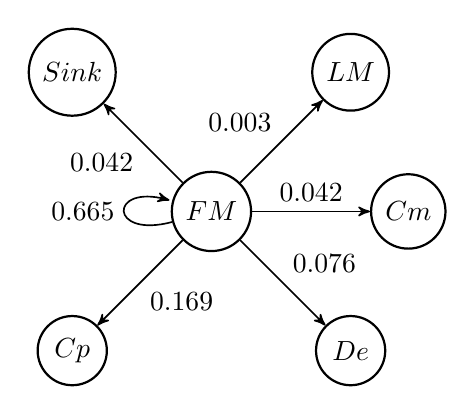
\begin{tikzpicture}[->, >=stealth', auto, semithick, node distance=2.5cm]
\tikzstyle{every state}=[fill=white,draw=black,thick,text=black,scale=1]
\node[state]    (A)                     {$FM$};
%\node[state]    (B)[above right of=A]   {$AS$};
%\node[state]    (C)[above left of=B]    {$Bl$};
%\node[state]    (D)[left of=C]          {$CS$};
%\node[state]    (E)[below right of=A]   {$CC$};
%\node[state]    (F)[below left of=E]    {$LC$};
%\node[state]    (G)[below right of=B]   {$LZC$};
%\node[state]    (H)[below right of =G]  {$LM$};
\node[state]    (H)[above right of =A]  {$LM$};
%\node[state]    (R)[below right of =H]  {$LP$};
%\node[state]    (I)[below left of=H]    {$MCh$};
%\node[state]    (J)[above right of=B]   {$RP$};
%\node[state]    (K)[above right of=G]   {$SC$};
%\node[state]    (L)[above of=B]         {$SG$};
%\node[state]    (M)[below right of=K]   {$SA$};
%\node[state]    (N)[above of=D]         {$Bu$};
%\node[state]    (O)[left of=D]          {$Source$};
%\node[state]    (P)[below right of=O]   {$Cm$};
\node[state]    (P)[right of=A]   {$Cm$};
%\node[state]    (Q)[below left of=P]   {$Cp$};
\node[state]    (Q)[below left of=A]   {$Cp$};
%\node[state]    (R)[below left of=A]    {$FM$};
%\node[state]    (S)[above right of=K]   {$Sink$};
\node[state]    (S)[above left of=A]   {$Sink$};
%\node[state]	(V)[below left of=O]	 {$De$};
\node[state]	(V)[below right of=A]	 {$De$};
%\node[state]    (U)[below right of=N]    {$Ob$};
%\node[state]    (Y)[above right of=O]   {$PT$};
%\node[state]    (Z)[above left of=O]   {$Si$};

\path
(A) edge[loop left]     node{$0.665$}   (A)
edge        node{$0.003$}       (H)
edge         node{$0.042$}      (P)
edge       node{$0.169$}        (Q)
edge        node{$0.076$}       (V)
edge         node{$0.042$}      (S);

\end{tikzpicture}
}
\caption{FactoryMethod (FM) mutation in Eclipse.}
\label{Figure:FM-Mutations-Eclipse}
\end{center}
\end{figure*}


\begin{figure}%[ht]
\begin{center}
\scalebox{0.7}{
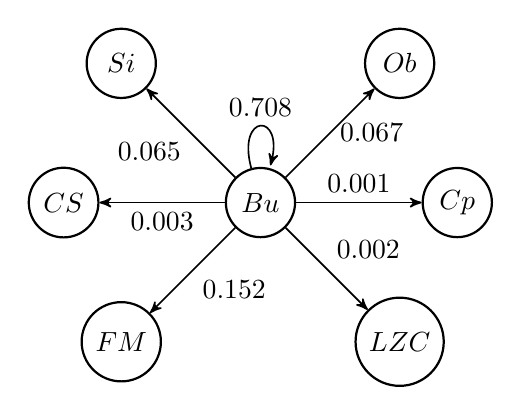
\begin{tikzpicture}[->, >=stealth', auto, semithick, node distance=2.5cm]
\tikzstyle{every state}=[fill=white,draw=black,thick,text=black,scale=1]
\node[state]    (A)                     {$Bu$};
%\node[state]    (B)[above right of=A]   {$AS$};
%\node[state]    (C)[above left of=B]    {$Bl$};
%\node[state]    (D)[left of=C]          {$CS$};
\node[state]    (D)[left of=A]          {$CS$};
%\node[state]    (E)[below right of=A]   {$CC$};
%\node[state]    (F)[below left of=E]    {$LC$};
%\node[state]    (G)[below right of=B]   {$LZC$};
\node[state]    (G)[below right of=A]   {$LZC$};
%\node[state]    (H)[below right of =G]  {$LM$};
%\node[state]    (R)[below right of =H]  {$LP$};
%\node[state]    (I)[below left of=H]    {$MCh$};
%\node[state]    (J)[above right of=B]   {$RP$};
%\node[state]    (K)[above right of=G]   {$SC$};
%\node[state]    (L)[above of=B]         {$SG$};
%\node[state]    (M)[below right of=K]   {$SA$};
%\node[state]    (N)[below left of=D]    {$Bu$};
%\node[state]    (O)[below left of=N]    {$Source$};
%\node[state]    (P)[below right of=O]   {$Cm$};
%\node[state]    (Q)[left of=A]          {$Cp$};
\node[state]    (Q)[right of=A]          {$Cp$};
%\node[state]    (R)[below left of=A]    {$FM$};
\node[state]    (R)[below left of=A]    {$FM$};
%\node[state]    (S)[above right of=K]   {$Sink$};
%\node[state]	(V)[right of=O]	        {$De$};
%\node[state]    (U)[below right of=N]   {$Ob$};
\node[state]    (U)[above right of=A]   {$Ob$};
%\node[state]    (Y)[above right of=O]   {$PT$};
\node[state]    (Z)[above left of=A]    {$Si$};

\path
(A) edge[loop above]     node{$0.708$}   (A)
edge        node{$0.003$}       (D)
edge         node{$0.002$}      (G)
edge       node{$0.001$}        (Q)
edge        node{$0.152$}       (R)
edge [right]        node{$0.067$}      (U)
edge        node{$0.065$}       (Z);

\end{tikzpicture}
}
\caption{Builder (Bu) mutation in Nuxeo.}
\label{Figure:Bu-Mutations-Nuxeo}
\end{center}
\end{figure} 

\begin{figure}
\begin{center}
\scalebox{0.7}{
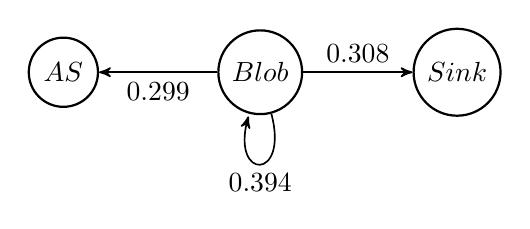
\begin{tikzpicture}[->, >=stealth', auto, semithick, node distance=2.5cm]
\tikzstyle{every state}=[fill=white,draw=black,thick,text=black,scale=1]
\node[state]    (A)                     {$Blob$};
\node[state]    (B)[left of=A]   {$AS$};
%\node[state]    (C)[above left of=B]    {$LP$};
%\node[state]    (D)[left of=C]          {$CS$};
%\node[state]    (E)[below right of=A]   {$CC$};
%\node[state]    (F)[below left of=E]    {$LC$};
%\node[state]    (G)[below right of=B]   {$LZC$};
%\node[state]    (H)[below right of =G]  {$LM$};
%\node[state]    (I)[below left of=H]    {$MCh$};
%\node[state]    (J)[above right of=B]   {$RP$};
%\node[state]    (K)[above right of=G]   {$SC$};
%\node[state]    (L)[above of=B]         {$SG$};
%\node[state]    (M)[below right of=K]   {$SA$};
%\node[state]    (N)[above of=D]         {$Bu$};
%\node[state]    (O)[left of=D]          {$Source$};
%\node[state]    (P)[below right of=O]   {$Cm$};
%\node[state]    (Q)[below left of=P]    {$Cp$};
%\node[state]    (R)[below left of=A]    {$FM$};
%\node[state]    (S)[above right of=K]   {$Sink$};
\node[state]    (S)[right of=A]   {$Sink$};
%\node[state]	(V)[below left of=R]	{$De$};
%\node[state]    (U)[below right of=N]    {$Ob$};
%\node[state]    (Y)[above right of=O]   {$PT$};
%\node[state]    (Z)[below left of=O]    {$Si$};

\path
(A) edge[loop below]     node{$0.394$}   (A)
edge        node{$0.299$}       (B)
edge         node{$0.308$}      (S);

\end{tikzpicture}
}
\caption{Blob (Bl) mutation in oVirt.}
\label{Figure:Bl-Mutations-Ovirt}
\end{center}
\end{figure}



\begin{figure*}
\begin{center}
\scalebox{0.8}{
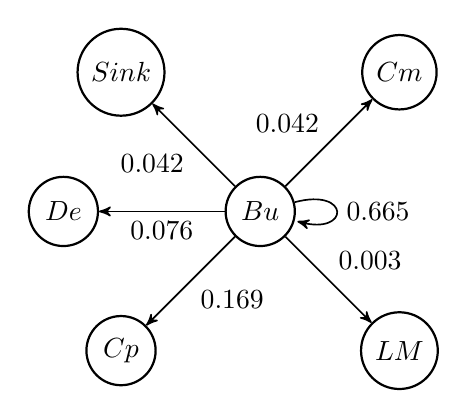
\begin{tikzpicture}[->, >=stealth', auto, semithick, node distance=2.5cm]
\tikzstyle{every state}=[fill=white,draw=black,thick,text=black,scale=1]
\node[state]    (A)                     {$Bu$};
%\node[state]    (B)[above right of=A]   {$AS$};
%\node[state]    (C)[above left of=B]    {$Bl$};
%\node[state]    (D)[left of=C]          {$CS$};
%\node[state]    (E)[below right of=A]   {$CC$};
%\node[state]    (F)[below left of=E]    {$LC$};
%\node[state]    (G)[below right of=B]   {$LZC$};
%\node[state]    (H)[below right of =G]  {$LM$};
\node[state]    (H)[below right of =A]  {$LM$};
%\node[state]    (R)[below right of =H]  {$LP$};
%\node[state]    (I)[below left of=H]    {$MCh$};
%\node[state]    (J)[above right of=B]   {$RP$};
%\node[state]    (K)[above right of=G]   {$SC$};
%\node[state]    (L)[above of=B]         {$SG$};
%\node[state]    (M)[below right of=K]   {$SA$};
%\node[state]    (N)[below left of=D]    {$Bu$};
%\node[state]    (O)[below left of=N]    {$Source$};
%\node[state]    (P)[below right of=O]   {$Cm$};
\node[state]    (P)[above right of=A]   {$Cm$};
%\node[state]    (Q)[below left of=P]   {$Cp$};
\node[state]    (Q)[below left of=A]   {$Cp$};
%\node[state]    (R)[below left of=A]    {$FM$};
%\node[state]    (S)[above right of=K]   {$Sink$};
\node[state]    (S)[above left of=A]   {$Sink$};
%\node[state]	(V)[right of=O]	        {$De$};
\node[state]	(V)[left of=A]	        {$De$};
%\node[state]    (U)[below right of=N]   {$Ob$};
%\node[state]    (Y)[above right of=O]   {$PT$};
%\node[state]    (Z)[above left of=O]    {$Si$};


\path
(A) edge[loop right]     node{$0.665$}   (A)
edge        node{$0.003$}       (H)
edge         node{$0.042$}      (P)
edge       node{$0.169$}        (Q)
edge        node{$0.076$}       (V)
edge         node{$0.042$}      (S);

\end{tikzpicture}
}
\caption{Builder (Bu) mutation among the different snapshots of Matsim.}
\label{Figure:Bu-Mutations-Matsim}
\end{center}
\end{figure*}

\begin{landscape}
\begin{table*}
\caption{Change probabilities of design anti-patterns and design patterns in oVirt}
\setlength\tabcolsep{0.08cm}% let LaTeX calculate intercolumn whitespace
\scriptsize
\centering
\scalebox{0.73}{
{\renewcommand{\arraystretch}{1.05}
\begin{tabular}
{|l|l||l|l|l|l|l|l|l|l|l|l|l|l|l||l|l|l|l|l|l|l|l||p{0.7cm}|p{0.9cm}}
\cline{2-24}
\multicolumn{1}{l|}{}& Source & AS & Bl & CS & CC & LC & LZC & LM & LP & MCh & RP & SC & SG & SA & Bu & Cm & Cp & FM & De & Ob & PT & Si & Sink \\
\hline
AS & 0.018 & \cellcolor[gray]{0.8}{\textbf{0.971}} & 0.000 & 0.000 & 0.000 & 0.000 & 0.000 & 0.000 & 0.000 & 0.000 & 0.000 & 0.000 & 0.000 & 0.000 & 0.000 & 0.000 & 0.000 & 0.000 & 0.000 & 0.000 & 0.000 & 0.000 & 0.011\\
\hline
Bl & 0.000 & \cellcolor[gray]{0.8}{\textbf{0.299}} & \cellcolor[gray]{0.8}{\textbf{0.394}} & 0.000 & 0.000 & 0.000 & 0.000 & 0.000 & 0.000 & 0.000 & 0.000 & 0.000 & 0.000 & 0.000 & 0.000 & 0.000 & 0.000 & 0.000 & 0.000 & 0.000 & 0.000 & 0.000 & \cellcolor[gray]{0.8}{\textbf{0.308}}\\
\hline
CS & 0.006 & 0.000 & 0.003 & \cellcolor[gray]{0.8}{\textbf{0.982}} & 0.000 & 0.000 & 0.000 & 0.000 & 0.000 & 0.000 & 0.000 & 0.000 & 0.000 & 0.000 & 0.000 & 0.000 & 0.000 & 0.000 & 0.000 & 0.000 & 0.000 & 0.000 & 0.009 \\
\hline
CC & 0.000 & 0.000 & 0.000 & 0.012 & \cellcolor[gray]{0.8}{\textbf{0.975}} & 0.000 & 0.000 & 0.000 & 0.000 & 0.000 & 0.000 & 0.000 & 0.000 & 0.000 & 0.000 & 0.000 & 0.000 & 0.000 & 0.000 & 0.000 & 0.000 & 0.000 & 0.013 \\
\hline
LC & 0.000 & 0.000 & 0.000 & 0.000 & 0.000 & \cellcolor[gray]{0.8}{\textbf{1}} & 0.000 & 0.000 & 0.000 & 0.000 & 0.000 & 0.000 & 0.000 & 0.000 & 0.000 & 0.000 & 0.000 & 0.000 & 0.000 & 0.000 & 0.000 & 0.000 & 0.000 \\
\hline
LZC & 0.000 & 0.000 & 0.000 & 0.000 & 0.000 & 0.001 & \cellcolor[gray]{0.8}{\textbf{0.998}} & 0.000 & 0.000 & 0.000 & 0.000 & 0.000 & 0.000 & 0.000 & 0.000 & 0.000 & 0.000 & 0.000 & 0.000 & 0.000 & 0.000 & 0.000 & 0.001 \\
\hline
LM & 0.000 & 0.000 & 0.000 & 0.000 & 0.000 & 0.000 & 0.012 & \cellcolor[gray]{0.8}{\textbf{0.977}} & 0.000 & 0.000 & 0.000 & 0.000 & 0.000 & 0.000 & 0.000 & 0.000 & 0.000 & 0.000 & 0.000 & 0.000 & 0.000 & 0.000 & 0.011 \\
\hline
LP & 0.000 & 0.000 & 0.000 & 0.000 & 0.000 & 0.000 & 0.000 & 0.008 & \cellcolor[gray]{0.8}{\textbf{0.969}} & 0.000 & 0.000 & 0.000 & 0.000 & 0.000 & 0.000 & 0.000 & 0.000 & 0.000 & 0.000 & 0.000 & 0.000 & 0.000 & 0.022 \\
\hline
MCh & 0.000 & 0.000 & 0.000 & 0.000 & 0.000 & 0.000 & 0.000 & 0.000 & 0.000 & \cellcolor[gray]{0.8}{\textbf{1}} & 0.000 & 0.000 & 0.000 & 0.000 & 0.000 & 0.000 & 0.000 & 0.000 & 0.000 & 0.000 & 0.000 & 0.000 & 0.000 \\
\hline
RP & 0.000 & 0.000 & 0.000 & 0.000 & 0.000 & 0.000 & 0.000 & 0.000 & 0.000 & 0.082 & \cellcolor[gray]{0.8}{\textbf{0.857}} & 0.000 & 0.000 & 0.000 & 0.000 & 0.000 & 0.000 & 0.000 & 0.000 & 0.000 & 0.000 & 0.000 & 0.061 \\
\hline
SC & 0.000 & 0.000 & 0.000 & 0.000 & 0.000 & 0.000 & 0.000 & 0.000 & 0.000 & 0.000 & 0.000 & \cellcolor[gray]{0.8}{\textbf{1}} & 0.000 & 0.000 & 0.000 & 0.000 & 0.000 & 0.000 & 0.000 & 0.000 & 0.000 & 0.000 & 0.000 \\
\hline 
SG & 0.000 & 0.000 & 0.000 & 0.000 & 0.000 & 0.000 & 0.000 & 0.000 & 0.000 & 0.000 & 0.000 & 0.000 & \cellcolor[gray]{0.8}{\textbf{1}} & 0.000 & 0.000 & 0.000 & 0.000 & 0.000 & 0.000 & 0.000 & 0.000 & 0.000 & 0.000\\
\hline
SA & 0.000 & 0.000 & 0.000 & 0.000 & 0.000 & 0.000 & 0.000 & 0.000 & 0.000 & 0.000 & 0.000 & 0.000 & 0.000 & \cellcolor[gray]{0.8}{\textbf{1}} & 0.000 & 0.000 & 0.000 & 0.000 & 0.000 & 0.000 & 0.000 & 0.000 & 0.000 \\
\hline \hline
Bu & 0.000 & 0.000 & 0.000 & 0.000 & 0.000 & 0.000 & 0.000 & 0.000 & 0.000 & 0.000 & 0.000 & 0.000 & 0.000 & 0.000 & \cellcolor[gray]{0.8}{\textbf{1}} & 0.000 & 0.000 & 0.000 & 0.000 & 0.000 & 0.000 & 0.000 & 0.000 \\
\hline 
Cm & 0.000 & 0.000 & 0.000 & 0.000 & 0.000 & 0.000 & 0.000 & 0.000 & 0.000 & 0.000 & 0.000 & 0.000 & 0.000 & 0.019 & 0.000 & \cellcolor[gray]{0.8}{\textbf{1}} & 0.000 & 0.000 & 0.000 & 0.000 & 0.000 & 0.000 & 0.000 \\
\hline
Cp & 0.000 & 0.000 & 0.000 & 0.000 & 0.000 & 0.000 & 0.000 & 0.000 & 0.000 & 0.000 & 0.000 & 0.000 & 0.000 & 0.000 & 0.000 & 0.000 & \cellcolor[gray]{0.8}{\textbf{1}} & 0.000 & 0.000 & 0.000 & 0.000 & 0.000 & 0.000 \\
\hline
FM & 0.000 & 0.000 & 0.000 & 0.000 & 0.000 & 0.000 & 0.000 & 0.000 & 0.000 & 0.000 & 0.000 & 0.000 & 0.000 & 0.000 & 0.000 & 0.000 & 0.000 & \cellcolor[gray]{0.8}{\textbf{1}} & 0.000 & 0.000 & 0.000 & 0.000 & 0.000 \\
\hline
De & 0.000 & 0.000 & 0.000 & 0.000 & 0.000 & 0.000 & 0.000 & 0.000 & 0.000 & 0.000 & 0.000 & 0.000 & 0.000 & 0.000 & 0.000 & 0.000 & 0.000 & 0.000 & \cellcolor[gray]{0.8}{\textbf{1}} & 0.000 & 0.000 & 0.000 & 0.000 \\
\hline
Ob & 0.000 & 0.000 & 0.000 & 0.000 & 0.000 & 0.000 & 0.000 & 0.000 & 0.000 & 0.000 & 0.000 & 0.000 & 0.000 & 0.000 & 0.000 & 0.000 & 0.000 & 0.000 & 0.000 & \cellcolor[gray]{0.8}{\textbf{1}} & 0.000 & 0.000 & 0.000 \\
\hline
PT & 0.000 & 0.000 & 0.000 & 0.000 & 0.000 & 0.000 & 0.000 & 0.000 & 0.000 & 0.000 & 0.000 & 0.000 & 0.000 & 0.000 & 0.000 & 0.000 & 0.000 & 0.000 & 0.000 & 0.000 & \cellcolor[gray]{0.8}{\textbf{1}} & 0.000 & 0.000 \\
\hline
Si & 0.000 & 0.001 & 0.000 & 0.000 & 0.000 & 0.000 & 0.000 & 0.000 & 0.000 & 0.000 & 0.000 & 0.000 & 0.000 & 0.000 & 0.000 & 0.000 & 0.000 & 0.000 & 0.000 & 0.000 & \cellcolor[gray]{0.8}{\textbf{0.097}} & \cellcolor[gray]{0.8}{\textbf{0.798}} & \cellcolor[gray]{0.8}{\textbf{0.103}} \\
\hline
\end{tabular}
}}
\label{tab:Ovirtmarkov}
\end{table*}

\begin{table*} %[ht] 
\caption{Change probabilities of design anti-patterns and design patterns in Matsim}
\setlength\tabcolsep{0.08cm}% let LaTeX calculate intercolumn whitespace
\scriptsize
\centering
\scalebox{0.73}{
{\renewcommand{\arraystretch}{1.05}
\begin{tabular}
{|l|l||l|l|l|l|l|l|l|l|l|l|l|l|l||l|l|l|l|l|l|l|l||p{0.7cm}|p{0.9cm}}
\cline{2-24}
\multicolumn{1}{l|}{}& Source & AS & Bl & CS & CC & LC & LZC & LM & LP & MCh & RP & SC & SG & SA & Bu & Cm & Cp & FM & De & Ob & PT & Si & Sink \\
\hline
AS & 0.066 & \cellcolor[gray]{0.8}{\textbf{0.893}} & 0.000 & 0.000 & 0.000 & 0.000 & 0.000 & 0.000 & 0.000 & 0.000 & 0.000 & 0.000 & 0.000 & 0.000 & 0.000 & 0.000 & 0.000 & 0.040 & 0.000 & 0.000 & 0.000 & 0.000 & 0.000\\
\hline
Bl & 0.003 & \cellcolor[gray]{0.8}{\textbf{0.372}} & \cellcolor[gray]{0.8}{\textbf{0.279}} & 0.000 & 0.000 & 0.000 & 0.000 & 0.000 & 0.000 & 0.000 & 0.000 & 0.000 & 0.000 & 0.000 & 0.000 & 0.000 & 0.000 & \cellcolor[gray]{0.8}{\textbf{0.346}} & 0.000 & 0.000 & 0.000 & 0.000 & 0.000\\
\hline
CS & 0.025 & 0.000 & 0.037 & \cellcolor[gray]{0.8}{\textbf{0.9}} & 0.000 & 0.000 & 0.000 & 0.000 & 0.000 & 0.000 & 0.000 & 0.000 & 0.000 & 0.000 & 0.000 & 0.000 & 0.000 & 0.038 & 0.000 & 0.000 & 0.000 & 0.000 & 0.000 \\
\hline
CC & 0.004 & 0.001 & 0.002 & 0.075 & \cellcolor[gray]{0.8}{\textbf{0.848}} & 0.000 & 0.000 & 0.000 & 0.000 & 0.000 & 0.000 & 0.000 & 0.000 & 0.000 & 0.000 & 0.000 & 0.000 & 0.069 & 0.000 & 0.000 & 0.000 & 0.000 & 0.000 \\
\hline
LC & 0.000 & 0.000 & 0.000 & 0.000 & 0.000 & \cellcolor[gray]{0.8}{\textbf{1}} & 0.000 & 0.000 & 0.000 & 0.000 & 0.000 & 0.000 & 0.000 & 0.000 & 0.000 & 0.000 & 0.000 & 0.000 & 0.000 & 0.000 & 0.000 & 0.000 & 0.000 \\
\hline
LZC & 0.000 & 0.003 & 0.000 & 0.000 & 0.000 & \cellcolor[gray]{0.8}{\textbf{0.1}} & \cellcolor[gray]{0.8}{\textbf{0.831}} & 0.000 & 0.000 & 0.000 & 0.000 & 0.000 & 0.000 & 0.000 & 0.000 & 0.000 & 0.000 & 0.066 & 0.000 & 0.000 & 0.000 & 0.000 & 0.000 \\
\hline
LM & 0.003 & 0.001 & 0.002 & 0.013 & 0.000 & 0.000 & 0.063 & \cellcolor[gray]{0.8}{\textbf{0.86}} & 0.000 & 0.000 & 0.000 & 0.000 & 0.000 & 0.000 & 0.000 & 0.000 & 0.000 & 0.059 & 0.000 & 0.000 & 0.000 & 0.000 & 0.000 \\
\hline
LP & 0.003 & 0.000 & 0.003 & 0.013 & 0.000 & 0.000 & 0.007 & 0.034 & \cellcolor[gray]{0.8}{\textbf{0.887}} & 0.000 & 0.000 & 0.000 & 0.000 & 0.000 & 0.000 & 0.000 & 0.000 & 0.053 & 0.000 & 0.000 & 0.000 & 0.000 & 0.000 \\
\hline
MCh & 0.000 & 0.000 & 0.000 & 0.000 & 0.000 & 0.000 & 0.000 & 0.000 & 0.000 & \cellcolor[gray]{0.8}{\textbf{1}} & 0.000 & 0.000 & 0.000 & 0.000 & 0.000 & 0.000 & 0.000 & 0.000 & 0.000 & 0.000 & 0.000 & 0.000 & 0.000 \\
\hline
RP & 0.000 & 0.000 & 0.000 & 0.000 & 0.000 & 0.000 & 0.000 & 0.000 & 0.000 & 0.021 & \cellcolor[gray]{0.8}{\textbf{0.596}} & 0.000 & 0.000 & 0.000 & 0.000 & 0.000 & 0.000 & \cellcolor[gray]{0.8}{\textbf{0.193}} & 0.000 & 0.000 & 0.000 & 0.000 & 0.000 \\
\hline
SC & 0.026 & 0.000 & 0.000 & 0.000 & 0.000 & 0.000 & 0.003 & 0.000 & 0.000 & 0.000 & 0.038 & \cellcolor[gray]{0.8}{\textbf{0.834}} & 0.000 & 0.000 & 0.000 & 0.000 & 0.000 & \cellcolor[gray]{0.8}{\textbf{0.099}} & 0.000 & 0.000 & 0.000 & 0.000 & 0.000 \\
\hline 
SG & 0.000 & 0.000 & 0.000 & 0.091 & 0.000 & 0.000 & 0.000 & 0.000 & 0.000 & 0.000 & 0.000 & \cellcolor[gray]{0.8}{\textbf{0.182}} & \cellcolor[gray]{0.8}{\textbf{0.455}} & 0.000 & 0.000 & 0.000 & 0.000 & \cellcolor[gray]{0.8}{\textbf{0.273}} & 0.000 & 0.000 & 0.000 & 0.000 & 0.000\\
\hline
SA & 0.000 & 0.000 & 0.000 & 0.000 & 0.000 & 0.000 & 0.000 & 0.000 & 0.000 & 0.000 & 0.000 & 0.000 & 0.000 & \cellcolor[gray]{0.8}{\textbf{1}} & 0.000 & 0.000 & 0.000 & 0.000 & 0.000 & 0.000 & 0.000 & 0.000 & 0.000 \\
\hline \hline
Bu & 0.000 & 0.000 & 0.000 & 0.001 & 0.000 & 0.000 & 0.003 & 0.000 & 0.000 & 0.000 & 0.000 & 0.000 & 0.000 & 0.000 & \cellcolor[gray]{0.8}{\textbf{0.546}} & 0.000 & 0.001 & \cellcolor[gray]{0.8}{\textbf{0.272}} & 0.000 & \cellcolor[gray]{0.8}{\textbf{0.141}} & 0.000 & 0.030 & 0.000 \\
\hline
Cm & 0.000 & 0.000 & 0.000 & 0.001 & 0.000 & 0.000 & 0.002 & 0.000 & 0.000 & 0.000 & 0.000 & 0.000 & 0.000 & 0.030 & 0.000 & \cellcolor[gray]{0.8}{\textbf{0.371}} & 0.075 & \cellcolor[gray]{0.8}{\textbf{0.387}} & \cellcolor[gray]{0.8}{\textbf{0.117}} & 0.012 & 0.000 & 0.000 & 0.000 \\
\hline
Cp & 0.000 & 0.000 & 0.000 & 0.002 & 0.000 & 0.000 & 0.003 & 0.000 & 0.000 & 0.000 & 0.000 & 0.000 & 0.000 & 0.000 & 0.037 & 0.044 & \cellcolor[gray]{0.8}{\textbf{0.850}} & 0.061 & 0.000 & 0.000 & 0.000 & 0.000 & 0.000 \\
\hline
FM & 0.000 & 0.000 & 0.000 & 0.001 & 0.000 & 0.000 & 0.001 & 0.001 & 0.000 & 0.000 & 0.000 & 0.000 & 0.000 & 0.000 & 0.000 & 0.036 & 0.074 & \cellcolor[gray]{0.8}{\textbf{0.825}} & 0.059 & 0.000 & 0.000 & 0.000 & 0.000 \\
\hline
De & 0.000 & 0.000 & 0.000 & 0.000 & 0.000 & 0.000 & 0.000 & 0.000 & 0.000 & 0.000 & 0.000 & 0.000 & 0.000 & 0.000 & 0.000 & 0.000 & 0.000 & 0.049 & \cellcolor[gray]{0.8}{\textbf{0.912}} & 0.034 & 0.000 & 0.000 & 0.000 \\
\hline
Ob & 0.000 & 0.000 & 0.000 & 0.000 & 0.000 & 0.000 & 0.000 & 0.000 & 0.000 & 0.000 & 0.000 & 0.000 & 0.000 & 0.000 & 0.000 & 0.000 & 0.000 & 0.000 & 0.000 & \cellcolor[gray]{0.8}{\textbf{1}} & 0.000 & 0.000 & 0.000 \\
\hline
PT & 0.000 & 0.000 & 0.000 & 0.000 & 0.000 & 0.000 & 0.000 & 0.000 & 0.000 & 0.000 & 0.000 & 0.000 & 0.000 & 0.000 & 0.000 & 0.000 & 0.000 & 0.000 & 0.000 & 0.000 & \cellcolor[gray]{0.8}{\textbf{1}} & 0.000 & 0.000 \\
\hline
Si & 0.000 & 0.000 & 0.000 & 0.000 & 0.000 & 0.000 & 0.001 & 0.000 & 0.000 & 0.000 & 0.000 & 0.000 & 0.000 & 0.000 & 0.000 & 0.000 & 0.000 & 0.028 & 0.000 & 0.000 & 0.009 & \cellcolor[gray]{0.8}{\textbf{0.962}} & 0.000 \\
\hline
\end{tabular}
}}
\label{tab:MatsimMarkov}
\end{table*}
\end{landscape}



% \begin{landscape}

% \end{landscape}


\begin{landscape}
\begin{table*}%[ht] 
\caption{Change probabilities of design anti-patterns and design patterns in ApacheSolr}
\setlength\tabcolsep{0.08cm}% let LaTeX calculate intercolumn whitespace
\scriptsize
\centering
\scalebox{0.73}{
{\renewcommand{\arraystretch}{1.05}
\begin{tabular}
{|l|l||l|l|l|l|l|l|l|l|l|l|l|l|l||l|l|l|l|l|l|l|l||p{0.9cm}|p{0.9cm}}
\cline{2-24}
\multicolumn{1}{l|}{}& Source & AS & Bl & CS & CC & LC & LZC & LM & LP & MCh & RP & SC & SG & SA & Bu & Cm & Cp & FM & De & Ob & PT & Si & Sink \\
\hline
AS & 0.000 & \cellcolor[gray]{0.8}{\textbf{1}} & 0.000 & 0.000 & 0.000 & 0.000 & 0.000 & 0.000 & 0.000 & 0.000 & 0.000 & 0.000 & 0.000 & 0.000 & 0.000 & 0.000 & 0.000 & 0.000 & 0.000 & 0.000 & 0.000 & 0.000 & 0.000 \\
\hline
Bl & 0.000 & \cellcolor[gray]{0.8}{\textbf{0.321}} & \cellcolor[gray]{0.8}{\textbf{0.365}} & 0.000 & 0.000 & 0.000 & 0.000 & 0.000 & 0.000 & 0.000 & 0.000 & 0.000 & 0.000 & 0.000 & 0.000 & 0.000 & 0.000 & 0.000 & 0.000 & 0.000 & 0.000 & 0.000 & \cellcolor[gray]{0.8}{\textbf{0.313}} \\
\hline
CS & 0.000 & 0.000 & 0.009 & \cellcolor[gray]{0.8}{\textbf{0.983}} & 0.000 & 0.000 & 0.000 & 0.000 & 0.000 & 0.000 & 0.000 & 0.000 & 0.000 & 0.000 & 0.000 & 0.000 & 0.000 & 0.000 & 0.000 & 0.000 & 0.000 & 0.000 & 0.008 \\
\hline
CC & 0.000 & 0.000 & 0.000 & 0.033 & \cellcolor[gray]{0.8}{\textbf{0.93}} & 0.000 & 0.000 & 0.000 & 0.000 & 0.000 & 0.000 & 0.000 & 0.000 & 0.000 & 0.000 & 0.000 & 0.000 & 0.000 & 0.000 & 0.000 & 0.000 & 0.000 & 0.037 \\
\hline
LC & 0.000 & 0.000 & 0.000 & 0.000 & 0.000 & \cellcolor[gray]{0.8}{\textbf{1}} & 0.000 & 0.000 & 0.000 & 0.000 & 0.000 & 0.000 & 0.000 & 0.000 & 0.000 & 0.000 & 0.000 & 0.000 & 0.000 & 0.000 & 0.000 & 0.000 & 0.000 \\
\hline
LZC & 0.000 & 0.000 & 0.000 & 0.000 & 0.000 & 0.072 & \cellcolor[gray]{0.8}{\textbf{0.859}} & 0.000 & 0.000 & 0.000 & 0.000 & 0.000 & 0.000 & 0.000 & 0.000 & 0.000 & 0.000 & 0.000 & 0.000 & 0.000 & 0.000 & 0.000 & 0.069 \\
\hline
LM & 0.000 & 0.000 & 0.001 & 0.002 & 0.000 & 0.000 & 0.033 & \cellcolor[gray]{0.8}{\textbf{0.928}} & 0.000 & 0.000 & 0.000 & 0.000 & 0.000 & 0.000 & 0.000 & 0.000 & 0.000 & 0.000 & 0.000 & 0.000 & 0.000 & 0.000 & 0.036 \\
\hline
LP & 0.000 & 0.001 & 0.000 & 0.008 & 0.000 & 0.000 & 0.007 & 0.079 & \cellcolor[gray]{0.8}{\textbf{0.779}} & 0.000 & 0.000 & 0.000 & 0.000 & 0.000 & 0.000 & 0.000 & 0.000 & 0.000 & 0.000 & 0.000 & 0.000 & 0.000 & 0.125 \\
\hline
MCh & 0.000 & 0.000 & 0.000 & 0.000 & 0.000 & 0.000 & 0.000 & 0.000 & 0.000 & \cellcolor[gray]{0.8}{\textbf{1}} & 0.000 & 0.000 & 0.000 & 0.000 & 0.000 & 0.000 & 0.000 & 0.000 & 0.000 & 0.000 & 0.000 & 0.000 & 0.000 \\
\hline
RP & 0.000 & 0.000 & 0.000 & 0.000 & 0.000 & 0.000 & 0.000 & 0.000 & 0.000 & 0.088 & \cellcolor[gray]{0.8}{\textbf{0.84}} & 0.000 & 0.000 & 0.000 & 0.000 & 0.000 & 0.000 & 0.000 & 0.000 & 0.000 & 0.000 & 0.000 & 0.072 \\
\hline
SC & 0.000 & 0.000 & 0.000 & 0.000 & 0.000 & 0.000 & 0.000 & 0.000 & 0.000 & 0.000 & 0.000 & \cellcolor[gray]{0.8}{\textbf{1}} & 0.000 & 0.000 & 0.000 & 0.000 & 0.000 & 0.000 & 0.000 & 0.000 & 0.000 & 0.000 & 0.000\\
\hline
SG & 0.000 & 0.000 & 0.000 & 0.000 & 0.000 & 0.000 & 0.000 & 0.000 & 0.000 & 0.000 & 0.013 & 0.000 &  \cellcolor[gray]{0.8}{\textbf{0.981}} & 0.000 & 0.000 & 0.000 & 0.000 & 0.000 & 0.000 & 0.000 & 0.000 & 0.000 & 0.006 \\
\hline
SA & 0.000 & 0.000 & 0.000 & 0.000 & 0.000 & 0.000 & 0.000 & 0.000 & 0.000 & 0.000 & 0.000 & 0.000 & 0.000 & \cellcolor[gray]{0.8}{\textbf{1}} & 0.000 & 0.000 & 0.000 & 0.000 & 0.000 & 0.000 & 0.000 & 0.000 & 0.000 \\
\hline \hline
Bu & 0.000 & 0.000 & 0.000 & 0.000 & 0.000 & 0.000 & 0.000 & 0.000 & 0.000 & 0.000 & 0.000 & 0.000 & 0.000 & 0.000 & \cellcolor[gray]{0.8}{\textbf{0.963}} & 0.000 & 0.000 & 0.000 & 0.000 & 0.005 & 0.000 & 0.000 & 0.027 \\
\hline
Cm & 0.000 & 0.000 & 0.000 & 0.000 & 0.000 & 0.000 & 0.000 & 0.000 & 0.000 & 0.000 & 0.000 & 0.000 & 0.000 & 0.000 & 0.000 & \cellcolor[gray]{0.8}{\textbf{1}} & 0.000 & 0.000 & 0.000 & 0.000 & 0.000 & 0.000 & 0.000 \\
\hline
Cp & 0.000 & 0.000 & 0.000 & 0.000 & 0.000 & 0.000 & 0.000 & 0.000 & 0.000 & 0.000 & 0.000 & 0.000 & 0.000 & 0.000 & 0.000 & 0.000 & \cellcolor[gray]{0.8}{\textbf{1}} & 0.000 & 0.000 & 0.000 & 0.000 & 0.000 & 0.000 \\
\hline
FM & 0.000 & 0.000 & 0.000 & 0.000 & 0.000 & 0.000 & 0.000 & 0.000 & 0.000 & 0.000 & 0.000 & 0.000 & 0.000 & 0.000 & 0.000 & 0.000 & 0.012 & \cellcolor[gray]{0.8}{\textbf{0.874}} & 0.005 & 0.000 & 0.000 & 0.000 & 0.092 \\
\hline
De & 0.000 & 0.000 & 0.000 & 0.000 & 0.000 & 0.000 & 0.000 & 0.000 & 0.000 & 0.000 & 0.000 & 0.000 & 0.000 & 0.000 & 0.000 & 0.000 & 0.000 & 0.000 & \cellcolor[gray]{0.8}{\textbf{0.996}} & 0.000 & 0.000 & 0.000 & 0.004 \\
\hline
Ob & 0.000 & 0.000 & 0.000 & 0.000 & 0.000 & 0.000 & 0.000 & 0.000 & 0.000 & 0.000 & 0.000 & 0.000 & 0.000 & 0.000 & 0.000 & 0.000 & 0.000 & 0.000 & 0.000 & \cellcolor[gray]{0.8}{\textbf{1}} & 0.000 & 0.000 & 0.000 \\
\hline
PT & 0.000 & 0.000 & 0.000 & 0.000 & 0.000 & 0.000 & 0.000 & 0.000 & 0.000 & 0.000 & 0.000 & 0.000 & 0.000 & 0.000 & 0.000 & 0.000 & 0.000 & 0.000 & 0.000 & 0.000 & \cellcolor[gray]{0.8}{\textbf{1}} & 0.000 & 0.000 \\
\hline
Si & 0.000 & 0.000 & 0.000 & 0.000 & 0.000 & 0.000 & 0.000 & 0.000 & 0.000 & 0.000 & 0.000 & 0.000 & 0.000 & 0.000 & 0.000 & 0.000 & 0.000 & 0.000 & 0.000 & 0.000 & 0.007 & \cellcolor[gray]{0.8}{\textbf{0.981}} & 0.012 \\
\hline
\end{tabular}
}
}
\label{tab:SolrMarkov}
\end{table*}

\begin{table*} %[ht]
\caption{Change probabilities of design anti-patterns and design patterns in ApacheIgnite}
\setlength\tabcolsep{0.08cm}% let LaTeX calculate intercolumn whitespace
\scriptsize
\centering
\scalebox{0.735}{
{\renewcommand{\arraystretch}{1.05}
\begin{tabular}
{|l|l||l|l|l|l|l|l|l|l|l|l|l|l|l||l|l|l|l|l|l|l|l||p{0.9cm}|p{0.9cm}}
\cline{2-24}
\multicolumn{1}{l|}{}& Source & AS & Bl & CS & CC & LC & LZC & LM & LP & MCh & RP & SC & SG & SA & Bu & Cm & Cp & FM & De & Ob & PT & Si & Sink \\
\hline
AS & 0.000 & \cellcolor[gray]{0.8}{\textbf{1}} & 0.000 & 0.000 & 0.000 & 0.000 & 0.000 & 0.000 & 0.000 & 0.000 & 0.000 & 0.000 & 0.000 & 0.000 & 0.000 & 0.000 & 0.000 & 0.000 & 0.000 & 0.000 & 0.000 & 0.000 & 0.000 \\
\hline
Bl & 0.000 & \cellcolor[gray]{0.8}{\textbf{0.375}} & \cellcolor[gray]{0.8}{\textbf{0.33}} & 0.000 & 0.000 & 0.000 & 0.000 & 0.000 & 0.000 & 0.000 & 0.000 & 0.000 & 0.000 & 0.000 & 0.000 & 0.000 & 0.000 & 0.000 & 0.000 & 0.000 & 0.000 & 0.000 & \cellcolor[gray]{0.8}{\textbf{0.295}} \\
\hline
CS & 0.000 & 0.000 & 0.000 & \cellcolor[gray]{0.8}{\textbf{1}} & 0.000 & 0.000 & 0.000 & 0.000 & 0.000 & 0.000 & 0.000 & 0.000 &  0.000 & 0.000 & 0.000 & 0.000 & 0.000 & 0.000 & 0.000 & 0.000 & 0.000 & 0.000 & 0.000 \\
\hline
CC & 0.000 & 0.000 & 0.000 & 0.053 & \cellcolor[gray]{0.8}{\textbf{0.905}} & 0.000 & 0.000 & 0.000 & 0.000 & 0.000 & 0.000 & 0.000 & 0.000 & 0.000 & 0.000 & 0.000 & 0.000 & 0.000 & 0.000 & 0.000 & 0.000 & 0.000 & 0.042 \\
\hline
LC & 0.000 & 0.000 & 0.000 & 0.000 & 0.000 & \cellcolor[gray]{0.8}{\textbf{1}} & 0.000 & 0.000 & 0.000 & 0.000 & 0.000 & 0.000 & 0.000 & 0.000 & 0.000 & 0.000 & 0.000 & 0.000 & 0.000 & 0.000 & 0.000 & 0.000 & 0.000 \\
\hline
LZC & 0.000 & 0.000 & 0.000 & 0.000 & 0.000 & 0.015 & \cellcolor[gray]{0.8}{\textbf{0.97}} & 0.000 & 0.000 & 0.000 & 0.000 & 0.000 & 0.000 & 0.000 & 0.000 & 0.000 & 0.000 & 0.000 & 0.000 & 0.000 & 0.000 & 0.000 & 0.015 \\
\hline
LM & 0.000 & 0.000 & 0.000 & 0.004 & 0.000 & 0.000 & 0.045 & \cellcolor[gray]{0.8}{\textbf{0.905}} & 0.000 & 0.000 & 0.000 & 0.000 & 0.000 & 0.000 & 0.000 & 0.000 & 0.000 & 0.000 & 0.000 & 0.000 & 0.000 & 0.000 & 0.047 \\
\hline
LP & 0.000 & 0.000 & 0.000 & 0.009 & 0.000 & 0.000 & 0.006 & 0.051 & \cellcolor[gray]{0.8}{\textbf{0.851}} & 0.000 & 0.000 & 0.000 & 0.000 & 0.000 & 0.000 & 0.000 & 0.000 & 0.000 & 0.000 & 0.000 & 0.000 & 0.000 & 0.081 \\
\hline
MCh & 0.000 & 0.000 & 0.000 & 0.000 & 0.000 & 0.000 & 0.000 & 0.000 & 0.000 & \cellcolor[gray]{0.8}{\textbf{1}} & 0.000 & 0.000 & 0.000 & 0.000 & 0.000 & 0.000 & 0.000 & 0.000 & 0.000 & 0.000 & 0.000 & 0.000 & 0.000 \\
\hline
RP & 0.000 & 0.000 & 0.000 & 0.000 & 0.000 & 0.000 & 0.000 & 0.000 & 0.000 & 0.000 & \cellcolor[gray]{0.8}{\textbf{1}} & 0.000 & 0.000 & 0.000 & 0.000 & 0.000 & 0.000 & 0.000 & 0.000 & 0.000 & 0.000 & 0.000 & 0.000 \\
\hline
SC & 0.000 & 0.000 & 0.000 & 0.000 & 0.000 & 0.000 & 0.000 & 0.000 & 0.000 & 0.000 & 0.000 & \cellcolor[gray]{0.8}{\textbf{1}} & 0.000 & 0.000 & 0.000 & 0.000 & 0.000 & 0.000 & 0.000 & 0.000 & 0.000 & 0.000 & 0.000 \\
\hline
SG & 0.000 & 0.000 & 0.000 & 0.000 & 0.000 & 0.000 & 0.000 & 0.000 & 0.000 & 0.000 & 0.000 & 0.000 & \cellcolor[gray]{0.8}{\textbf{1}} & 0.000 & 0.000 & 0.000 & 0.000 & 0.000 & 0.000 & 0.000 & 0.000 & 0.000 & 0.000 \\
\hline
SA & 0.000 & 0.000 & 0.000 & 0.000 & 0.000 & 0.000 & 0.000 & 0.000 & 0.000 & 0.000 & 0.000 & 0.000 & 0.000 & \cellcolor[gray]{0.8}{\textbf{1}} & 0.000 & 0.000 & 0.000 & 0.000 & 0.000 & 0.000 & 0.000 & 0.000 & 0.000 \\
\hline \hline
Bu & 0.000 & 0.000 & 0.000 & 0.000 & 0.000 & 0.000 & 0.000 & 0.000 & 0.000 & 0.000 & 0.000 & 0.000 & 0.000 & 0.000 & \cellcolor[gray]{0.8}{\textbf{0.976}} & 0.000 & 0.000 & 0.000 & 0.000 & 0.004 & 0.000 & 0.000 & 0.018 \\
\hline
Cm & 0.000 & 0.000 & 0.000 & 0.000 & 0.000 & 0.000 & 0.000 & 0.000 & 0.000 & 0.000 & 0.000 & 0.000 & 0.000 & 0.000 & 0.000 & \cellcolor[gray]{0.8}{\textbf{1}} & 0.000 & 0.000 & 0.000 & 0.000 & 0.000 & 0.000 & 0.000 \\
\hline
Cp & 0.000 & 0.000 & 0.000 & 0.000 & 0.000 & 0.000 & 0.000 & 0.000 & 0.000 & 0.000 & 0.000 & 0.000 & 0.000 & 0.000 & 0.000 & 0.000 & \cellcolor[gray]{0.8}{\textbf{1}} & 0.000 & 0.000 & 0.000 & 0.000 & 0.000 & 0.000 \\
\hline
FM & 0.000 & 0.000 & 0.000 & 0.000 & 0.000 & 0.000 & 0.000 & 0.000 & 0.000 & 0.000 & 0.000 & 0.000 & 0.000 & 0.000 & 0.000 & 0.000 & 0.000 & \cellcolor[gray]{0.8}{\textbf{1}} & 0.000 & 0.000 & 0.000 & 0.000 & 0.000 \\
\hline
De & 0.000 & 0.000 & 0.000 & 0.000 & 0.000 & 0.000 & 0.000 & 0.000 & 0.000 & 0.000 & 0.000 & 0.000 & 0.000 & 0.000 & 0.000 & 0.000 & 0.000 & 0.000 & \cellcolor[gray]{0.8}{\textbf{1}} & 0.000 & 0.000 & 0.000 & 0.000 \\
\hline
Ob & 0.000 & 0.000 & 0.000 & 0.000 & 0.000 & 0.000 & 0.000 & 0.000 & 0.000 & 0.000 & 0.000 & 0.000 & 0.000 & 0.000 & 0.000 & 0.000 & 0.000 & 0.000 & 0.000 & \cellcolor[gray]{0.8}{\textbf{1}} & 0.000 & 0.000 & 0.000 \\
\hline
PT & 0.000 & 0.000 & 0.000 & 0.000 & 0.000 & 0.000 & 0.000 & 0.000 & 0.000 & 0.000 & 0.000 & 0.000 & 0.000 & 0.000 & 0.000 & 0.000 & 0.000 & 0.000 & 0.000 & 0.000 & \cellcolor[gray]{0.8}{\textbf{1}} & 0.000 & 0.000 \\
\hline
Si & 0.000 & 0.000 & 0.000 & 0.000 & 0.000 & 0.000 & 0.000 & 0.000 & 0.000 & 0.000 & 0.000 & 0.000 & 0.000 & 0.000 & 0.000 & 0.000 & 0.000 & 0.000 & 0.000 & 0.000 & 0.003 & \cellcolor[gray]{0.8}{\textbf{0.994}} & 0.003 \\
\hline
\end{tabular}
}}
\label{tab:IgniteMarkov}
\end{table*}

\end{landscape}


\begin{landscape}
\begin{table*}
\caption{Change probabilities of design anti-patterns and design patterns in Mule}
\setlength\tabcolsep{0.08cm}% let LaTeX calculate intercolumn whitespace
\scriptsize
\centering
\scalebox{0.73}{
{\renewcommand{\arraystretch}{1.05}
\begin{tabular}
{|l|l||l|l|l|l|l|l|l|l|l|l|l|l|l||l|l|l|l|l|l|l|l||p{0.7cm}|p{0.9cm}}
\cline{2-24}
\multicolumn{1}{l|}{}& Source & AS & Bl & CS & CC & LC & LZC & LM & LP & MCh & RP & SC & SG & SA & Bu & Cm & Cp & FM & De & Ob & PT & Si & Sink \\
\hline
AS & 0.032 & \cellcolor[gray]{0.8}{\textbf{0.937}} & 0.000 & 0.000 & 0.000 & 0.000 & 0.000 & 0.000 & 0.000 & 0.000 & 0.000 & 0.000 & 0.000 & 0.000 & 0.000 & 0.000 & 0.000 & 0.030 & 0.000 & 0.000 & 0.000 & 0.000 & 0.000\\
\hline
Bl & 0.000 & \cellcolor[gray]{0.8}{\textbf{0.313}} & \cellcolor[gray]{0.8}{\textbf{0.313}} & 0.000 & 0.000 & 0.000 & 0.000 & 0.000 & 0.000 & 0.000 & 0.000 & 0.000 & 0.000 & 0.000 & 0.000 & 0.000 & 0.000 & \cellcolor[gray]{0.8}{\textbf{0.374}} & 0.000 & 0.000 & 0.000 & 0.000 & 0.000\\
\hline
CS & 0.003 & 0.000 & 0.006 & \cellcolor[gray]{0.8}{\textbf{0.963}} & 0.000 & 0.000 & 0.000 & 0.000 & 0.000 & 0.000 & 0.000 & 0.000 & 0.000 & 0.000 & 0.000 & 0.000 & 0.000 & 0.028 & 0.000 & 0.000 & 0.000 & 0.000 & 0.000 \\
\hline
CC & 0.001 & 0.000 & 0.000 & 0.071 & \cellcolor[gray]{0.8}{\textbf{0.843}} & 0.000 & 0.000 & 0.000 & 0.000 & 0.000 & 0.000 & 0.000 & 0.000 & 0.000 & 0.000 & 0.000 & 0.000 & 0.084 & 0.000 & 0.000 & 0.000 & 0.000 & 0.000 \\
\hline
LC & 0.000 & 0.000 & 0.000 & 0.000 & 0.000 & \cellcolor[gray]{0.8}{\textbf{1}} & 0.000 & 0.000 & 0.000 & 0.000 & 0.000 & 0.000 & 0.000 & 0.000 & 0.000 & 0.000 & 0.000 & 0.000 & 0.000 & 0.000 & 0.000 & 0.000 & 0.000 \\
\hline
LZC & 0.000 & 0.000 & 0.000 & 0.000 & 0.000 & 0.030 & \cellcolor[gray]{0.8}{\textbf{0.946}} & 0.000 & 0.000 & 0.000 & 0.000 & 0.000 & 0.000 & 0.000 & 0.000 & 0.000 & 0.000 & 0.024 & 0.000 & 0.000 & 0.000 & 0.000 & 0.000 \\
\hline
LM & 0.000 & 0.000 & 0.000 & 0.010 & 0.000 & 0.000 & 0.039 & \cellcolor[gray]{0.8}{\textbf{0.907}} & 0.000 & 0.000 & 0.000 & 0.000 & 0.000 & 0.000 & 0.000 & 0.000 & 0.000 & 0.044 & 0.000 & 0.000 & 0.000 & 0.000 & 0.000 \\
\hline
LP & 0.000 & 0.000 & 0.000 & 0.014 & 0.000 & 0.000 & 0.009 & \cellcolor[gray]{0.8}{\textbf{0.115}} & \cellcolor[gray]{0.8}{\textbf{0.676}} & 0.000 & 0.000 & 0.000 & 0.000 & 0.000 & 0.000 & 0.000 & 0.000 & \cellcolor[gray]{0.8}{\textbf{0.186}} & 0.000 & 0.000 & 0.000 & 0.000 & 0.000 \\
\hline
MCh & 0.000 & 0.000 & 0.000 & 0.000 & 0.000 & 0.000 & 0.000 & 0.000 & 0.000 & \cellcolor[gray]{0.8}{\textbf{1}} & 0.000 & 0.000 & 0.000 & 0.000 & 0.000 & 0.000 & 0.000 & 0.000 & 0.000 & 0.000 & 0.000 & 0.000 & 0.000 \\
\hline
RP & 0.000 & 0.000 & 0.000 & 0.033 & 0.000 & 0.000 & 0.067 & 0.000 & 0.000 & \cellcolor[gray]{0.8}{\textbf{0.233}} & \cellcolor[gray]{0.8}{\textbf{0.233}} & 0.000 & 0.000 & 0.000 & 0.000 & 0.000 & 0.000 & \cellcolor[gray]{0.8}{\textbf{0.433}} & 0.000 & 0.000 & 0.000 & 0.000 & 0.000 \\
\hline
SC & \cellcolor[gray]{0.8}{\textbf{0.096}} & 0.000 & 0.000 & 0.000 & 0.000 & 0.000 & 0.000 & 0.000 & 0.000 & 0.000 & 0.074 & \cellcolor[gray]{0.8}{\textbf{0.649}} & 0.000 & 0.000 & 0.000 & 0.000 & 0.000 & \cellcolor[gray]{0.8}{\textbf{0.181}} & 0.000 & 0.000 & 0.000 & 0.000 & 0.000 \\
\hline 
SG & 0.000 & 0.000 & 0.000 & 0.000 & 0.000 & 0.000 & 0.000 & 0.000 & 0.000 & 0.000 & 0.000 & 0.053 & \cellcolor[gray]{0.8}{\textbf{0.947}} & 0.000 & 0.000 & 0.000 & 0.000 & 0.000 & 0.000 & 0.000 & 0.000 & 0.000 & 0.000\\
\hline
SA & 0.000 & 0.000 & 0.000 & 0.000 & 0.000 & 0.000 & 0.000 & 0.000 & 0.000 & 0.000 & 0.000 & 0.000 & 0.000 & \cellcolor[gray]{0.8}{\textbf{1}} & 0.000 & 0.000 & 0.000 & 0.000 & 0.000 & 0.000 & 0.000 & 0.000 & 0.000 \\
\hline \hline
Bu & 0.000 & 0.000 & 0.000 & 0.003 & 0.000 & 0.000 & 0.002 & 0.000 & 0.000 & 0.000 & 0.000 & 0.000 & 0.000 & 0.000 & \cellcolor[gray]{0.8}{\textbf{0.708}} & 0.000 & 0.001 & \cellcolor[gray]{0.8}{\textbf{0.152}} & 0.000 & 0.067 & 0.000 & 0.065 & 0.000 \\
\hline
Cm & 0.000 & 0.000 & 0.000 & 0.003 & 0.000 & 0.000 & 0.000 & 0.000 & 0.000 & 0.000 & 0.000 & 0.000 & 0.000 & 0.019 & 0.000 & \cellcolor[gray]{0.8}{\textbf{0.687}} & \cellcolor[gray]{0.8}{\textbf{0.096}} & \cellcolor[gray]{0.8}{\textbf{0.193}} & 0.000 & 0.000 & 0.000 & 0.000 & 0.000 \\
\hline
Cp & 0.000 & 0.000 & 0.000 & 0.002 & 0.000 & 0.000 & 0.002 & 0.000 & 0.000 & 0.000 & 0.000 & 0.000 & 0.000 & 0.000 & 0.000 & 0.058 & \cellcolor[gray]{0.8}{\textbf{0.882}} & 0.054 & 0.000 & 0.000 & 0.000 & 0.000 & 0.000 \\
\hline
FM & 0.000 & 0.000 & 0.000 & 0.003 & 0.000 & 0.000 & 0.002 & 0.000 & 0.000 & 0.000 & 0.000 & 0.000 & 0.000 & 0.000 & 0.000 & 0.042 & 0.087 & \cellcolor[gray]{0.8}{\textbf{0.764}} & \cellcolor[gray]{0.8}{\textbf{0.099}} & 0.000 & 0.000 & 0.000 & 0.000 \\
\hline
De & 0.000 & 0.000 & 0.000 & 0.001 & 0.000 & 0.000 & 0.000 & 0.000 & 0.000 & 0.000 & 0.000 & 0.000 & 0.000 & 0.000 & 0.000 & 0.000 & 0.000 & 0.014 & \cellcolor[gray]{0.8}{\textbf{0.971}} & 0.013 & 0.000 & 0.000 & 0.000 \\
\hline
Ob & 0.000 & 0.000 & 0.000 & 0.000 & 0.000 & 0.000 & 0.000 & 0.000 & 0.000 & 0.000 & 0.000 & 0.000 & 0.000 & 0.000 & 0.000 & 0.000 & 0.000 & 0.024 & 0.024 & \cellcolor[gray]{0.8}{\textbf{0.951}} & 0.000 & 0.000 & 0.000 \\
\hline
PT & 0.000 & 0.000 & 0.000 & 0.000 & 0.000 & 0.000 & 0.000 & 0.000 & 0.000 & 0.000 & 0.000 & 0.000 & 0.000 & 0.000 & 0.000 & 0.000 & 0.000 & 0.000 & 0.000 & 0.000 & \cellcolor[gray]{0.8}{\textbf{1}} & 0.000 & 0.000 \\
\hline
Si & 0.000 & 0.000 & 0.000 & 0.001 & 0.000 & 0.000 & 0.000 & 0.000 & 0.000 & 0.000 & 0.000 & 0.000 & 0.000 & 0.000 & 0.000 & 0.000 & 0.000 & 0.029 & 0.000 & 0.000 & 0.006 & \cellcolor[gray]{0.8}{\textbf{0.964}} & 0.000 \\
\hline
\end{tabular}
}}
\label{tab:Mulemarkov}
\end{table*}

\begin{table*}
\caption{Change probabilities of design anti-patterns and design patterns in all studied systems}
\setlength\tabcolsep{0.08cm}
\scriptsize
\centering
\scalebox{0.73}{
{\renewcommand{\arraystretch}{1.05}
\begin{tabular}
{|l|l||l|l|l|l|l|l|l|l|l|l|l|l|l||l|l|l|l|l|l|l|l||l|p{0.7cm}|p{0.9cm}}
\cline{2-24}
\multicolumn{1}{l|}{}& Source & AS & Bl & CS & CC & LC & LZC & LM & LP & MCh & RP & SC & SG & SA & Bu & Cm & Cp & FM & De & Ob & PT & Si & Sink \\
\hline
AS & 0.022 & \cellcolor[gray]{0.8}{\textbf{0.961}} & 0.000 & 0.000 & 0.000 & 0.000 & 0.000 & 0.000 & 0.000 & 0.000 & 0.000 & 0.000 & 0.000 & 0.000 & 0.000 & 0.000 & 0.000 & 0.010 & 0.000 & 0.000 & 0.000 & 0.000 & 0.005 \\
\hline
Bl & 0.001 & \cellcolor[gray]{0.8}{\textbf{0.309}} & \cellcolor[gray]{0.8}{\textbf{0.378}} & 0.000 & 0.000 & 0.000 & 0.000 & 0.000 & 0.000 & 0.000 & 0.000 & 0.000 & 0.000 & 0.000 & 0.000 & 0.000 & 0.000 & 0.092 & 0.000 & 0.000 & 0.000 & 0.000 & \cellcolor[gray]{0.8}{\textbf{0.218}} \\
\hline
CS & 0.006 & 0.000 & 0.008 & \cellcolor[gray]{0.8}{\textbf{0.971}} & 0.000 & 0.000 & 0.000 & 0.000 & 0.000 & 0.000 & 0.000 & 0.000 & 0.000 & 0.000 & 0.000 & 0.000 & 0.000 & 0.008 & 0.000 & 0.000 & 0.000 & 0.000 & 0.005 \\
\hline
CC & 0.000 & 0.000 & 0.000 & 0.029 & \cellcolor[gray]{0.8}{\textbf{0.936}} & 0.000 & 0.000 & 0.000 & 0.000 & 0.000 & 0.000 & 0.000 & 0.000 & 0.000 & 0.000 & 0.000 & 0.000 & 0.019 & 0.000 & 0.000 & 0.000 & 0.000 & 0.014 \\
\hline
LC & 0.000 & 0.000 & 0.000 & 0.000 & \cellcolor[gray]{0.8}{\textbf{0.5}} & \cellcolor[gray]{0.8}{\textbf{0.5}} & 0.000 & 0.000 & 0.000 & 0.000 & 0.000 & 0.000 & 0.000 & 0.000 & 0.000 & 0.000 & 0.000 & 0.000 & 0.000 & 0.000 & 0.000 & 0.000 & 0.000 \\
\hline
LZC & 0.000 & 0.000 & 0.000 & 0.000 & 0.000 & 0.011 & \cellcolor[gray]{0.982}{\textbf{0.979}} & 0.000 & 0.000 & 0.000 & 0.000 & 0.000 & 0.000 & 0.000 & 0.000 & 0.000 & 0.000 & 0.003 & 0.000 & 0.000 & 0.000 & 0.000 & 0.005 \\
\hline
LM & 0.000 & 0.000 & 0.000 & 0.003 & 0.000 & 0.000 & 0.028 & \cellcolor[gray]{0.8}{\textbf{0.937}} & 0.000 & 0.000 & 0.000 & 0.000 & 0.000 & 0.000 & 0.000 & 0.000 & 0.000 & 0.015 & 0.000 & 0.000 & 0.000 & 0.000 & 0.012 \\
\hline
LP & 0.000 & 0.000 & 0.000 & 0.003 & 0.000 & 0.000 & 0.002 & 0.022 & \cellcolor[gray]{0.8}{\textbf{0.929}} & 0.000 & 0.000 & 0.000 & 0.000 & 0.000 & 0.000 & 0.000 & 0.000 & 0.013 & 0.000 & 0.000 & 0.000 & 0.000 & 0.028 \\
\hline
MCh & 0.000 & 0.000 & 0.000 & 0.000 & 0.000 & 0.000 & 0.000 & 0.000 & 0.000 & \cellcolor[gray]{0.8}{\textbf{1}} & 0.000 & 0.000 & 0.000 & 0.000 & 0.000 & 0.000 & 0.000 & 0.000 & 0.000 & 0.000 & 0.000 & 0.000 & 0.000 \\
\hline
RP & 0.000 & 0.000 & 0.000 & 0.001 & 0.000 & 0.000 & 0.002 & 0.000 & 0.000 & \cellcolor[gray]{0.8}{\textbf{0.115}} & \cellcolor[gray]{0.8}{\textbf{0.770}} & 0.000 & 0.000 & 0.000 & 0.000 & 0.000 & 0.000 & 0.052 & 0.000 & 0.000 & 0.000 & 0.000 & 0.056 \\
\hline
SC & 0.031 & 0.000 & 0.000 & 0.031 & 0.000 & 0.000 & 0.001 & 0.000 & 0.000 & 0.000 & 0.049 & \cellcolor[gray]{0.8}{\textbf{0.811}} & 0.000 & 0.000 & 0.000 & 0.000 & 0.000 & \cellcolor[gray]{0.8}{\textbf{0.102}} & 0.000 & 0.000 & 0.000 & 0.000 & 0.000 \\
\hline 
SG & 0.000 & 0.000 & 0.000 & 0.005 & 0.000 & 0.000 & 0.000 & 0.000 & 0.000 & 0.000 & 0.010 & 0.015 & \cellcolor[gray]{0.8}{\textbf{0.947}} & 0.000 & 0.000 & 0.000 & 0.000 & 0.015 & 0.000 & 0.000 & 0.000 & 0.000 & 0.005 \\
\hline
SA & 0.000 & 0.000 & 0.000 & 0.000 & 0.000 & 0.000 & 0.000 & 0.000 & 0.000 & 0.000 & 0.000 & 0.000 & 0.000 & \cellcolor[gray]{0.8}{\textbf{1}} & 0.000 & 0.000 & 0.000 & 0.000 & 0.000 & 0.000 & 0.000 & 0.000 & 0.000 \\ \hline\hline
%\Xhline {1.5pt}
Bu & 0.000 & 0.000 & 0.000 & 0.000 & 0.000 & 0.000 & 0.001 & 0.000 & 0.000 & 0.000 & 0.000 & 0.000 & 0.000 & 0.000 & \cellcolor[gray]{0.8}{\textbf{0.150}} & 0.000 & 0.003 & \cellcolor[gray]{0.8}{\textbf{0.509}} & 0.000 & \cellcolor[gray]{0.8}{\textbf{0.323}} & 0.000 & 0.009 & 0.000 \\
\hline
Cm & 0.000 & 0.000 & 0.000 & 0.001 & 0.000 & 0.000 & 0.004 & 0.000 & 0.000 & 0.000 & 0.000 & 0.000 & 0.000 & 0.001 & 0.000 & \cellcolor[gray]{0.8}{\textbf{0.146}} & \cellcolor[gray]{0.8}{\textbf{0.239}} & \cellcolor[gray]{0.8}{\textbf{0.566}} & 0.017 & 0.021 & 0.000 & 0.000 & 0.000 \\
\hline
Cp & 0.000 & 0.000 & 0.000 & 0.002 & 0.000 & 0.000 & 0.005 & 0.000 & 0.000 & 0.000 & 0.000 & 0.000 & 0.000 & 0.000 & 0.002 & 0.072 & \cellcolor[gray]{0.8}{\textbf{0.838}} & 0.078 & 0.000 & 0.000 & 0.000 & 0.000 & 0.000 \\
\hline
FM & 0.000 & 0.000 & 0.000 & 0.000 & 0.002 & 0.000 & 0.000 & 0.001 & 0.001 & 0.000 & 0.000 & 0.000 & 0.000 & 0.000 & 0.000 & 0.023 & \cellcolor[gray]{0.8}{\textbf{0.111}} & \cellcolor[gray]{0.8}{\textbf{0.814}} & 0.043 & 0.000 & 0.000 & 0.000 & 0.000 \\
\hline
De & 0.000 & 0.001 & 0.001 & 0.002 & 0.000 & 0.002 & 0.000 & 0.001 & 0.000 & 0.000 & 0.000 & 0.000 & 0.000 & 0.000 & 0.000 & 0.000 & 0.000 & \cellcolor[gray]{0.8}{\textbf{0.144}} & \cellcolor[gray]{0.8}{\textbf{0.734}} & \cellcolor[gray]{0.8}{\textbf{0.108}} & 0.000 & 0.000 & 0.000 \\
\hline
Ob & 0.015 & 0.000 & 0.000 & 0.000 & 0.000 & 0.000 & 0.000 & 0.000 & 0.000 & 0.000 & 0.000 & 0.000 & 0.000 & 0.000 & 0.000 & 0.000 & 0.000 & 0.095 &\cellcolor[gray]{0.8}{\textbf{0.126}} & \cellcolor[gray]{0.8}{\textbf{0.761}} & 0.000 & 0.000 & 0.000 \\
\hline
PT & 0.000 & 0.001 & 0.000 & 0.000 & 0.000 & 0.000 & 0.000 & 0.000 & 0.000 & 0.000 & 0.000 & 0.000 & 0.000 & 0.000 & 0.000 & 0.000 & 0.000 & 0.000 & 0.000 & 0.000 & \cellcolor[gray]{0.8}{\textbf{1}} & 0.000 & 0.000 \\
\hline
Si & 0.000 & 0.000 & 0.000 & 0.000 & 0.000 & 0.000 & 0.000 & 0.000 & 0.000 & 0.000 & 0.000 & 0.000 & 0.000 & 0.000 & 0.000 & 0.000 & 0.000 & 0.013 & 0.000 & 0.000 & 0.013 & \cellcolor[gray]{0.8}{\textbf{0.966}} & 0.006 \\
\hline
\end{tabular}
}}
\label{tab:AllSystems}
\end{table*}
\end{landscape}

\begin{figure*} %[ht]
\begin{center}
\scalebox{0.7}{
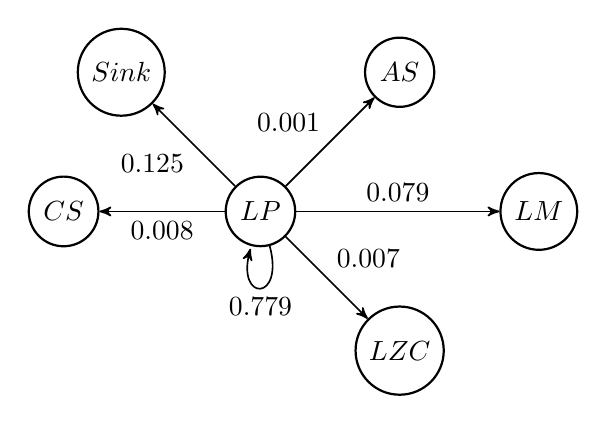
\begin{tikzpicture}[->, >=stealth', auto, semithick, node distance=2.5cm]
\tikzstyle{every state}=[fill=white,draw=black,thick,text=black,scale=1]
\node[state]    (A)                     {$LP$};
%\node[state]    (B)[above right of=A]   {$AS$};
\node[state]    (B)[above right of=A]   {$AS$};
%\node[state]    (C)[above left of=B]    {$Bl$};
%\node[state]    (D)[left of=C]          {$CS$};
\node[state]    (D)[left of=A]          {$CS$};
%\node[state]    (E)[below right of=A]   {$CC$};
%\node[state]    (F)[below left of=E]    {$LC$};
%\node[state]    (G)[below right of=B]   {$LZC$};
\node[state]    (G)[below right of=A]   {$LZC$};
%\node[state]    (H)[below right of =G]  {$LM$};
\node[state]    (H)[below right of =B]  {$LM$};
%\node[state]    (I)[below left of=H]    {$MCh$};
%\node[state]    (J)[above right of=B]   {$RP$};
%\node[state]    (K)[above right of=G]   {$SC$};
%\node[state]    (L)[above of=B]         {$SG$};
%\node[state]    (M)[below right of=K]   {$SA$};
%\node[state]    (N)[above of=D]         {$Bu$};
%\node[state]    (O)[left of=D]          {$Source$};
%\node[state]    (P)[below right of=O]   {$Cm$};
%\node[state]    (Q)[below left of=P]    {$Cp$};
%\node[state]    (R)[below left of=A]    {$FM$};
%\node[state]    (S)[above right of=K]   {$Sink$};
\node[state]    (S)[above left of=A]   {$Sink$};
%\node[state]	(V)[below left of=R]	{$De$};
%\node[state]    (U)[below right of=N]    {$Ob$};
%\node[state]    (Y)[above right of=O]   {$PT$};
%\node[state]    (Z)[below left of=O]    {$Si$};

\path
(A) edge[loop below]     node{$0.779$}   (A)
edge        node{$0.001$}       (B)
edge         node{$0.008$}      (D)
edge       node{$0.007$}        (G)
edge        node{$0.079$}       (H)
edge         node{$0.125$}      (S);

\end{tikzpicture}
}
\caption{LongParameterList (LP) mutation in ApacheSolr.}
\label{Figure:LP-Mutations-ApacheSolr}
\end{center}
\end{figure*}


\begin{figure*} %[ht]
\begin{center}
\scalebox{0.7}{
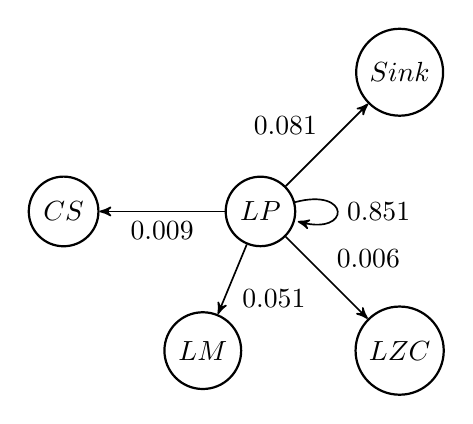
\begin{tikzpicture}[->, >=stealth', auto, semithick, node distance=2.5cm]
\tikzstyle{every state}=[fill=white,draw=black,thick,text=black,scale=1]
\node[state]    (A)                     {$LP$};
%\node[state]    (B)[above right of=A]   {$AS$};
%\node[state]    (C)[above left of=B]    {$Bl$};
%\node[state]    (D)[left of=C]          {$CS$};
\node[state]    (D)[left of=A]          {$CS$};
%\node[state]    (E)[below right of=A]   {$CC$};
%\node[state]    (F)[below left of=E]    {$LC$};
%\node[state]    (G)[below right of=B]   {$LZC$};
\node[state]    (G)[below right of=A]   {$LZC$};
%\node[state]    (H)[below right of =G]  {$LM$};
\node[state]    (H)[below right of =D]  {$LM$};
%\node[state]    (I)[below left of=H]    {$MCh$};
%\node[state]    (J)[above right of=B]   {$RP$};
%\node[state]    (K)[above right of=G]   {$SC$};
%\node[state]    (L)[above of=B]         {$SG$};
%\node[state]    (M)[below right of=K]   {$SA$};
%\node[state]    (N)[above of=D]         {$Bu$};
%\node[state]    (O)[left of=D]          {$Source$};
%\node[state]    (P)[below right of=O]   {$Cm$};
%\node[state]    (Q)[below left of=P]    {$Cp$};
%\node[state]    (R)[below left of=A]    {$FM$};
%\node[state]    (S)[above right of=K]   {$Sink$};
\node[state]    (S)[above right of=A]  {$Sink$};
%\node[state]	(V)[below left of=R]	{$De$};
%\node[state]    (U)[below right of=N]   {$Ob$};
%\node[state]    (Y)[above right of=O]   {$PT$};
%\node[state]    (Z)[below left of=O]    {$Si$};

\path
(A) edge[loop right]     node{$0.851$}   (A)
edge         node{$0.009$}      (D)
edge       node{$0.006$}        (G)
edge        node{$0.051$}       (H)
edge         node{$0.081$}      (S);

\end{tikzpicture}
}
\caption{LongParameterList (LP) mutation in ApacheIgnite.}
\label{Figure:LP-Mutations-ApacheIgnite}
\end{center}
\end{figure*}

\begin{figure}
\begin{center}
\scalebox{0.8}{
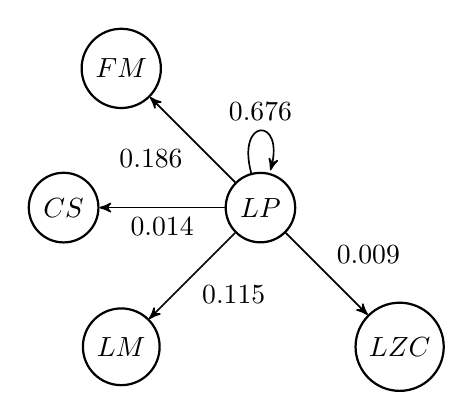
\begin{tikzpicture}[->, >=stealth', auto, semithick, node distance=2.5cm]
\tikzstyle{every state}=[fill=white,draw=black,thick,text=black,scale=1]
\node[state]    (A)                     {$LP$};
%\node[state]    (B)[above right of=A]   {$AS$};
%\node[state]    (C)[above left of=B]    {$Bl$};
%\node[state]    (D)[left of=C]          {$CS$};
\node[state]    (D)[left of=A]          {$CS$};
%\node[state]    (E)[below right of=A]   {$CC$};
%\node[state]    (F)[below left of=E]    {$LC$};
%\node[state]    (G)[below right of=B]   {$LZC$};
\node[state]    (G)[below right of=A]   {$LZC$};
%\node[state]    (H)[below right of =G]  {$LM$};
\node[state]    (H)[below left of =A]  {$LM$};
%\node[state]    (I)[below left of=H]    {$MCh$};
%\node[state]    (J)[above right of=B]   {$RP$};
%\node[state]    (K)[above right of=G]   {$SC$};
%\node[state]    (L)[above of=B]         {$SG$};
%\node[state]    (M)[below right of=K]   {$SA$};
%\node[state]    (N)[above of=D]         {$Bu$};
%\node[state]    (O)[left of=D]          {$Source$};
%\node[state]    (P)[below right of=O]   {$Cm$};
%\node[state]    (Q)[below left of=P]    {$Cp$};
%\node[state]    (R)[below left of=A]    {$FM$};
\node[state]    (R)[above left of=A]    {$FM$};
%\node[state]    (S)[above right of=K]   {$Sink$};
%\node[state]	(V)[below left of=R]	{$De$};
%\node[state]    (U)[below right of=N]    {$Ob$};
%\node[state]    (Y)[above right of=O]   {$PT$};
%\node[state]    (Z)[below left of=O]    {$Si$};

\path
(A) edge[loop above]     node{$0.676$}   (A)
%edge        node{$0.001$}       (B)
edge         node{$0.014$}      (D)
edge         node{$0.009$}      (G)
edge         node{$0.115$}      (H)
edge         node{$0.186$}      (R);

\end{tikzpicture}
}
\caption{LongParameterList (LP) mutation in Mule.}
\label{Figure:LP-Mutations-Mule}
\end{center}
\end{figure}



Tables \ref{tab:EclipseMarkov} to \ref{tab:Mulemarkov} show the mutations between design patterns and design anti-patterns that occurred in their evolutions. Table \ref{tab:AllSystems} aggregates all the mutations in all the systems. We added two additional states (source and sink) to describe the appearances of design (anti-)patterns (sources) and the disappearance of some design (anti-)patterns (sinks).

% A \textit{Source} indicates the new classes which did not participate in the occurrences of design patterns and--or design anti-patterns before the selected period of evolution. A \textit{sink}, on the other hand, represents the classes which participated in occurrences of design patterns and--or design anti-patterns during the selected period of evolution but not after.

\begin{table*} %[ht]
\centering
\caption{Standard deviation values and confidence levels}
\scalebox{0.9}{
\renewcommand{\arraystretch}{1.05}
\begin{math}
\begin{tabular}{|l|r|r|r|}
\hline
\textbf{Systems} & \textbf{Standard Deviation} & \textbf{Confidence Level} & \textbf{Margin of Error}\\
 \hline \hline
 Apache Ignite & 0.1966 & 90\%, 1.645 $\sigma x$ & 0.04347$\pm$0.0147 ($\pm$33.87\%)\\ 
 \hline
 Apache Solr & 0.1921 & 90\%, 1.645 $\sigma x$ & 0.04343$\pm$0.0144 ($\pm$33.12\%) \\
 \hline
 Eclipse & 0.1833 & 90\%, 1.645 $\sigma x$ & 0.04317$\pm$0.0137 ($\pm$31.79\%) \\
\hline
 Matsim & 0.1722 & 90\%, 1.645 $\sigma x$ & 0.04304 $\pm$0.0129 ($\pm$29.96\%) \\
\hline
 Mule & 0.1766 & 90\%, 1.645 $\sigma x$ & 0.04345 $\pm$0.0132($\pm$30.43\%) \\
\hline
 Nuxeo & 0.1968 & 90\%, 1.645 $\sigma x$ & 0.0451 $\pm$0.0147 ($\pm$32.67\%) \\
\hline
 oVirt & 0.1961 & 90\%, 1.645 $\sigma x$ & 0.04352 $\pm$0.0147 ($\pm$33.73\%) \\
\hline
\end{tabular}
\end{math}
}
\label{tab:standardDeviation}
\end{table*}

The mutation probabilities shown in previous tables are percentages that may hide outliers. Therefore, we also calculate the standard deviation values among these probabilities. 
%Low standard deviation values mean that most of the numbers are close to the average while a high standard deviation values mean that the numbers are spread out.
We found that the probabilities across snapshots have low standard-deviation values, as shown in Table \ref{tab:standardDeviation}, with the highest value of 0.196 for Nuxeo. 

% These low standard-deviation values indicate that the values shown in the tables are representative of their trends and that we can be confident in the conclusion drawn from them.

Table \ref{tab:standardDeviation} shows a systematic analysis of the confidence levels of our results. We computed the standard-deviation values and confidence intervals of our results for a confidence level of 90\% as follows:

\begin{equation}
    \sigma = \sqrt{\frac{1}{N}\sum_{i=1}^{N}{ (x_i-\mu)}^2}
\end{equation}

\noindent where $x_i$ is each value from the population (mutations probabilities), $\mu$ is the mean of the population, and $N$ is the size of the population, \ie{} the total number of mutations in all the snapshots of a system.

With the standard deviation known, we compute the confidence interval for a population mean as:

\begin{equation}
    \bar{X}\pm Z \times {\frac{\sigma}{\sqrt{N}}}
\end{equation}

\noindent where $\bar{X}$ is plus or minus a margin of error, $Z$ is the Z-value for the chosen confidence level, $\sigma$ is a standard deviation and $N$ is the size of the population.

We observe that, for a confidence level of 90\%, the confidence intervals, which indicate how much we can expect the results to reflect the observations from the overall population, were around 30\% in all the analysed systems. We consider these values of confidence levels and intervals acceptable to deduce trends and infer conclusions. Indeed, while we could not find similar discussions and numbers in other software-engineering papers, we observed similar values used to deduce trends in other domains, \eg{} public health \cite{strazzullo2009salt}.

\begin{table*} %[ht]
\centering
\caption{Mean values of the mutations of design anti-patterns and design pattern occurrences mutated in all the snapshots of each system}
\scalebox{0.8}{
\renewcommand{\arraystretch}{1.1}
\begin{math}
\begin{tabular}{|l|r|r|}
\hline
\textbf{Systems} & \textbf{Mean Value of DAPs mutations} & \textbf{Mean Value of DPs mutations} \\
 \hline \hline
 Apache Ignite & 0.0799 & 0.0037 \\ 
 \hline
 Apache Solr & 0.1026 & 0.0232 \\
 \hline
 Eclipse & 0.1355 & 0.1128 \\
\hline
 Matsim & 0.2013 & 0.1917 \\
\hline
 Mule & 0.1989 & 0.1341 \\
\hline
 Nuxeo & 0.0848 & 0.03 \\
\hline
 oVirt & 0.0674 & 0.0252 \\
\hline
\end{tabular}
\end{math}
}
\label{tab:MeanValue}
\end{table*} 

For example, SpaghettiCode has the most representative mutation probability from Source in Mule (see Table \ref{tab:Mulemarkov}) and Blob to Sink in Apache Solr (see Table \ref{tab:SolrMarkov}). Table \ref{tab:mostrp} shows the most representative design patterns and design anti-patterns regarding mutation probabilities to/from other patterns.

\begin{table*} %[ht]
\centering
\renewcommand {\arraystretch} {1.1}
\caption{Most representative mutations between design patterns and design anti-patterns according to their mutation probabilities}
\scalebox{0.7}{
\begin{tabular}{|p{1.75cm}|l|l|l|r|}
\hline
\textbf{System} & \textbf{Mutation Type} & \textbf{From}  & \textbf{To} & \textbf{Probability} \\ \hline
\hline
\multirow{4}{*}{Apache Ignite} & DAP$\,\to\,$DAP & Blob (Bl) & AntiSingleton (AS) & 0.375\\
\cline{2-5}
& DAP$\,\to\,$DP & - & - & -\\
\cline{2-5}
  & DP$\,\to\,$DAP & - & - & -\\
  \cline{2-5}
   & DP$\,\to\,$DP & Builder (Bu) & Observer (ob) & 0.004\\
  \cline{2-5}
\hline
\multirow{4}{*}{Apache Solr} & DAP$\,\to\,$DAP & Blob (Bl) & AntiSingleton (AS) & 0.321\\
\cline{2-5}
& DAP$\,\to\,$DP & - & - & -\\
\cline{2-5}
& DP$\,\to\,$DAP & - & - & -\\
\cline{2-5}
& DP$\,\to\,$DP & FactoryMethod (FM) & Composite (Cp) & 0.012\\
\hline 
\multirow{4}{*}{Eclipe IDE} & DAP$\,\to\,$DAP & LargeClass (LC) & ComplexClass (Cc) & 0.500\\
\cline{2-5}
 & DAP$\,\to\,$DP & - & - & -\\
\cline{2-5}
 & DP$\,\to\,$DAP & FactoryMethod (FM) & LongMethod (LM) & 0.003\\
\cline{2-5}
 & DP$\,\to\,$DP & FactoryMethod (FM) & Composite (Cp) & 0.169\\
\hline 
\multirow{4}{*}{Matsim} & DAP$\,\to\,$DAP & Blob (Bl) & AntiSingleton (AS) & 0.372\\
\cline{2-5}
 & DAP$\,\to\,$DP & Blob (Bl) & FactoryMethod (FM) & 0.346\\
\cline{2-5}
 & DP$\,\to\,$DAP & Command (Cm) & SwissArmyKnife (SA) & 0.030\\
\cline{2-5}
 & DP$\,\to\,$DP & Command (Cm) & FactoryMethod (FM) & 0.387\\
\hline 
\multirow{4}{*}{Mule} & DAP$\,\to\,$DAP & Blob (bl) & AntiSingleton(AS) & 0.313\\
\cline{2-5}
 & DAP$\,\to\,$DP & RefusedParentBequest (RP) & FactoryMethod (FM) & 0.433\\
\cline{2-5}
 & DP$\,\to\,$DAP & Command (Cm) & SwissArmyKnife (SA) & 0.019\\
\cline{2-5}
 & DP$\,\to\,$DP & Command (Cm) & FactoryMethod & 0.193\\
\hline 
\multirow{4}{*}{Nuxeo} & DAP$\,\to\,$DAP & Blob (bl) & AntiSingleton(AS) & 0.283\\
\cline{2-5}
 & DAP$\,\to\,$DP & Blob (Bl) & FactoryMethod (FM) & 0.297\\
\cline{2-5}
 & DP$\,\to\,$DAP & Singleton (Si) & LazyClass (ZC) & 0.004\\
\cline{2-5}
 & DP$\,\to\,$DP & Singleton (Si) & FactoryMethod (FM) & 0.133\\
\hline 
\multirow{4}{*}{ovirt} & DAP$\,\to\,$DAP & Blob (bl) & AntiSingleton(AS) & 0.299\\
\cline{2-5}
 & DAP$\,\to\,$DP & - & - & -\\
\cline{2-5}
 & DP$\,\to\,$DAP & Singleton (Si) & AntiSingleton (AS) & 0.001\\
\cline{2-5}
 & DP$\,\to\,$DP & Singleton (Si) & Prototype (PT) & 0.097\\
\hline 
\end{tabular}
}
\label{tab:mostrp}
\end{table*} 

\paragraph{\textbf{Analysing pattern evolution}} We observe in Table \ref{tab:mostrp} that not all design patterns and design anti-pattern undergo changes. Some patterns remain stable during evolution. For example, LazyClass and MessageChain are stable design anti-patterns, while Prototype is a persistent design pattern in Apache Solr. In Matsim, design anti-patterns SwissArmyKnife, LazyClass, and MessageChain and design patterns Observer and ProtoType are stable.

However, in general, design anti-patterns tend to evolve in all studied systems. We observe that more than half of the design anti-patterns mutated into other design patterns or design anti-patterns across the different snapshots of the studied system. 

For example, in Matsim (see Table \ref{tab:MatsimMarkov}), 86\% (probability value 0.86) LongMethod remains stable and mutate with only a probability of 14\% into other patterns. In oVirt (see Table \ref{tab:Ovirtmarkov}), Blob remain persistent in the system with 39.4\% probability, while 29.9\% mutated to AntiSingleton and into other patterns with a probability of 30.8\%. As last example, in Eclipse, 45.5\% of RefusedParentBequest remain between snapshot while 27.3\% mutated to MessageChain and 27.3\% mutated into other patterns.

We saw fewer mutations among design patterns. As an example, in Apache Ignite, 97.6\% of Command remained stable, with only 0.4\% mutating into other patterns.

% In general, we believe that mutations happen when developers solve design and coding problems. They modify the code and--or apply design patterns to these problems. Yet, they can also introduce design anti-patterns or other, undesired design pattern.

% We built Markov models to compute the probabilities of design anti-patterns and design patterns appearing, disappearing, and mutating during software evolution. We studied seven systems with different sizes to generalize our findings.

For a better understanding of the design pattern and design anti-pattern mutations, Figures \ref{Figure:FM-Mutations-Eclipse} to \ref{Figure:LP-Mutations-Mule} show the most representative mutations in the Markov models as graphs, for each of the systems. Because showing all possible probabilities would make the graphs unreadable, we choose a threshold of 0.100 to reduce the number of edges in each graph. The gray cells in Tables \ref{tab:EclipseMarkov} to  \ref{tab:Mulemarkov} highlight the probabilities shown in the figures. (The graphs for all the mutations in all the systems are available on-line\footnote{\url{http://www.ptidej.net/downloads/replications/emse19c/}}.)

These graphs contain information on mutating design (anti-)patterns that can help developers to avoid the mutations that could have negative impacts on software quality. 

\begin{tcolorbox}
\vspace{-0.1cm}
\textbf{Summary:} Our results show that design patterns and design anti-patterns mutate during the evolution of software systems. Despite an average of less than 20\% of the identified design anti-patterns occurrences having mutated among all the snapshots of systems, more than half of the types of design anti-patterns were involved in these mutations. For example, Table \ref{tab:MeanValue} shows that, in Matsim, 20.13\% of the design anti-pattern identified  in the first snapshot mutated during the studied period. During that period, ten types of design anti-patterns out of the 13 considered in our study were involved in mutations. In most of the systems, almost all the design patterns remained stable during evolution. Blob and Command are the design anti-patterns and design pattern with the higher mutation probabilities.
\vspace{-0.1cm}
\end{tcolorbox}



\subsection{\textbf{RQ2:} \textit{\RQTwo}}

\paragraph{\textbf{Motivation}} Knowing the causes of design (anti-)patterns mutations would be useful during maintenance. They could help developers to focus on the most frequent change types triggering patterns mutations. 

% Thus, we identify the types of changes to understand why and how design patterns and--or design anti-patterns mutate between two successive snapshots.  

\paragraph{\textbf{Analysing change types}} We use srcML\footnote{https://www.srcml.org/} to create an XML file for each snapshot of a system and match their tags to find changed tags, as explained in Section \ref{ssec:section3.6}. We categorise change types based on our categories in Table \ref{tab:Change_types}. We compare the percentages of each change type for each system. We apply the same methodology for all the subject systems.
Figures \ref{fig:FigureChangeEclipseNew} to \ref{fig:FigureChangeMuleNew} show the types of changes per design (anti-)patterns per systems. 

Table \ref{tab:Changes} presents the numbers of each change types in all the systems. For example, in Apache Ignite, we observe that Access and  Renaming are the least and most representative change types for both design patterns and design anti-patterns. They lead to many changes in occurrences of both design anti-patterns and design patterns.

\begin{landscape}
\begin{center}
	\begin{table*}
		\renewcommand {\arraystretch} {1.05}
		\centering
		
		\caption{Number of different types of changes in design patterns and design anti-patterns\label{tab:Changes}}
		\scalebox{0.61}{
		%\begin{tabular}{|p{2.05cm}|p{0.55cm}|p{0.55cm}|p{0.6cm}|p{0.4cm}|p{0.7cm}|p{0.4cm}|p{0.7cm}|p{0.7cm}|p{0.55cm}|p{0.45cm}|p{0.55cm}|p{0.35cm}|p{0.55cm}|p{0.55cm}|} \hline
		\begin{tabular}{|p{2.7cm}|r|r|r|r|r|r|r|r|r|r|r|r|r|r|} \hline
			\textbf{Systems~$\rightarrow$} & \multicolumn{2}{c}{\textbf{Eclipse}}& \multicolumn{2}{|c}{\textbf{Nuxeo}} & \multicolumn{2}{|c}{\textbf{oVirt}}& \multicolumn{2}{|c}{\textbf{Matsim}}&\multicolumn{2}{|c}{\textbf{Apache Solr}}&\multicolumn{2}{|c}{\textbf{Apache Ignite}}&\multicolumn{2}{|c|}{\textbf{Mule}}\\ \hline 
			\multirow{2}{*}{\textbf{Change Types~$\downarrow$}}
			& 1~~~ & 2~~~ & 3~~~ & 4~~~ & 5~~~ & 6~~~ & 7~~~ & 8~~~ & 9~~~ & 10~~ & 11~~ & 12~~ & 13~~ & 14~~\\ \cline{2-15} 
			& \textbf{DAP}~~ & \textbf{DP}~~ & \textbf{DAP}~~ & \textbf{DP}~~  & \textbf{DAP}~~ & \textbf{DP}~~ & \textbf{DAP}~~ & \textbf{DP}~~ & \textbf{DAP}~~ & \textbf{DP}~~ & \textbf{DAP}~~ & \textbf{DP}~~ & \textbf{DAP}~~ & \textbf{DP}~~\\ \hline \hline
			Access & 33 & 6 & 85 & 0 & 174 & 9 & 271 & 117 & 34	& 15 & 11 & 55 & 20&12	\\ \hline
			Class & 268 & 91 & 236 & 6 & 3804 & 90 & 1697 &	690 & 721 & 155 & 781&218 & 443&198 \\ \hline
			Code block & 4197 &	1075 & 1070	& 13 & 13923 &	233 & 8805 & 3203 &	3873 & 459 & 3903&203 &1430 &413	\\ \hline 
			Comment & 32939 & 11388	& 9269	& 109 &	15013 &	411 & 22519	& 9287 & 9298 &	2616 & 14554& 1567& 6354&3780	\\ \hline 
			Control Flow & 10487 & 1870	& 966 &	10 & 6440 &	118 & 5398	& 2094 & 3166 & 636 & 3433 & 133 &916 &384	\\ \hline 
			Declaration & 9721 & 2789 &	3133 & 24 &	 27605 & 487 & 24244 & 9609 & 8803 & 1392 & 9527& 349 &3904 &1103	\\ \hline 
			Exception & 996 & 341 &	946 & 1	& 619 &	29 & 1602 &	314 & 1696 & 457 & 2076& 64& 505&173	    \\ \hline
			Import & 2566 &	835 & 2734	& 23 & 18819 & 211 & 13013 & 4679 &	4024 & 491 & 4584& 394&3234 &793	    \\ \hline
			Invocation & 1707 & 394	& 556 & 4 & 7312 & 91 &	8520 & 3026	& 2598	& 287 & 2069 & 75 &945 &240	    \\ \hline
			Method & 4060 &	942 & 1487	& 29 & 13792 & 292 & 4702 &	1922 & 3215	& 511 & 3364 & 266 & 1940&747	\\ \hline 
			Operator & 13540 & 2803	& 3533	& 8	& 35513	& 403 &	57112 &	24326 &	7963 & 702 & 7207& 525& 5241&1975	\\ \hline 
			Parameter & 5629 & 1541	& 2179	& 3 & 24488	& 292 &	22080 &	5149 & 8375 & 1069  & 9024& 332&3252 &756	\\ \hline 
			Renaming & 59254 & 14707 & 16259 & 23 &	262491 &3536 &294661&145720& 44422 & 4811 & 63961& 4396&28110&9738	\\ \hline 
			\textbf{\#Changed classes} & 10957 & 3155 & 5402& 81 & 34780 & 55 & 32596 & 13768 & 7956& 1192 & 9290& 857& 5684&2175	\\ \hline
			\textbf{Total classes} & 20331 &	7574 &	39051 &	1263 & 142537 & 2482 & 62272 & 79480 & 32332 & 5490 & 27080 & 5796 & 47146&17553	\\ \hline
			\multicolumn{15}{c}{\textbf{AP, DP}= Number of changes in design anti-patterns and design patterns respectively}\\ \hline	
		\end{tabular}
		}
	\end{table*}
	
	\begin{table*}
		\centering
		\renewcommand {\arraystretch} {1.05}
		\caption{Number of different types of changes in design patterns and design anti-patterns mutation.\label{tab:dpapMutations}}
		%\begin{tabular}{|p{2cm}|p{0.57cm}|p{0.57cm}|p{0.57cm}|p{0.57cm}|p{0.57cm}|p{0.57cm}|p{0.57cm}|p{0.57cm}|p{0.57cm}|p{0.57cm}|p{0.57cm}|p{0.57cm}|p{0.57cm}|p{0.57cm}|} \hline
		%	Systems$\rightarrow$ & \multicolumn{2}{c}{Eclipse}& \multicolumn{2}{|c}{Nuxeo} & \multicolumn{2}{|c}{Ovirt}& \multicolumn{2}{|c}{Matsim}&\multicolumn{2}{|c|}{Apache Solr}&\multicolumn{2}{|c|}{Apache Ignite}&\multicolumn{2}{|c|}{Mule}\\ \hline 
		%	\multirow{2}{*}{Change Types~$\downarrow$}
		%	& 1 & 2 & 3 & 4 & 5 & 6 & 7 & 8 & 9 & 10 & 11 & 12& 13 & 14\\ \cline{2-15}
		\scalebox{0.58}{
		\begin{tabular}{|p{2.5cm}|r|r|r|r|r|r|r|r|r|r|r|r|r|r|} \hline
			\textbf{Systems$\rightarrow$} & \multicolumn{2}{c}{\textbf{Eclipse}}& \multicolumn{2}{|c}{\textbf{Nuxeo}} & \multicolumn{2}{|c}{\textbf{oVirt}}& \multicolumn{2}{|c}{\textbf{Matsim}}&\multicolumn{2}{|c}{\textbf{Apache Solr}}&\multicolumn{2}{|c}{\textbf{Apache Ignite}}&\multicolumn{2}{|c|}{\textbf{Mule}}\\ \hline 
			\multirow{2}{*}{\textbf{Change Types~$\downarrow$}}
			& 1~~~~ & 2~~~~ & 3~~~~ & 4~~~~ & 5~~~~ & 6~~~~ & 7~~~~ & 8~~~~ & 9~~~~ & 10~~~ & 11~~~ & 12~~~ & 13~~~ & 14~~~\\ \cline{2-15} 
			 & \textbf{APDP} & \textbf{DPAP} & \textbf{APDP} & \textbf{DPAP} & \textbf{APDP} & \textbf{DPAP} & \textbf{APDP} & \textbf{DPAP} & \textbf{APDP} & \textbf{DPAP} & \textbf{APDP} & \textbf{DPAP} & \textbf{APDP} & \textbf{DPAP}\\ \hline \hline
			Access & 0 & 0 &0 & 1 &1 &1 &0 &12 &3 &0 &0 &0 &0 &1	\\ \hline
			Class & 3&1	&2	&0	&10	&0	&4 &29	&1	&7 &2 &4 &6 &3 \\ \hline
			Code block & 1 &2 &1 &4	&21	&22	&10	&132 &4	&1 &1 &3 &27 &17	\\ \hline 
			Comment & 102&192	&7	&4	&69	&31	&38	&739 &129 &242 &58 &23 &160 &85	\\ \hline 
			Control Flow & 28&38&0	&3	&7	&6	&12	&96	&44	&31	 &16 &4 &21 &3	\\ \hline 
			Declaration & 56 & 78 & 3 &2 &82 &38 &56 &412 &141 &90 &33 &16 &49 &32	\\ \hline 
			Exception & 4&6	&0	&0	&4	&1	&6	&28	&19	&13	&14 &4 &3 &2	    \\ \hline
			Import & 20&14	&3 &2	&32	&18	&28	&257 &60 &34 &17 &16 &28 &18	    \\ \hline
			Invocation & 6&	7&0	&0	&15	&20	&7	&183 &1	&6	&5 &6 & 10&3	    \\ \hline
			Method & 16&18	&2	&2	&41	&24	&7	&96	&64	&43	 &10 &12 &23 &13	\\ \hline 
			Operator & 38&37 &2	&0	&43	&66	&95	&523 &22 &20 &6 &13 &87 &32	\\ \hline 		
			Parameter & 22 & 41 & 0 & 0	&37	&20	&16	&423 &25 &47 &22 &29 &13 &22	\\ \hline 
			Renaming & 675&	469&3 &2 &297 &1036	&462 &5096	&165 &406 &100 &63 &334 &280	\\ \hline 
			\#Changed classes& 71 & 77 & 7 & 6	& 61 & 54 &58 &681 &58	&66	 &34 &29 &53 &39	\\ \hline
			\multicolumn{15}{c}{\textbf{APDP, DPAP}= Number of changes in design anti-patterns to design patterns and design patterns to design anti-patterns mutations respectively}\\ \hline
		\end{tabular}
		}
	\end{table*}
\end{center}
\end{landscape}

% Eclipse
\begin{figure}
\centering
\scalebox{1.1}{
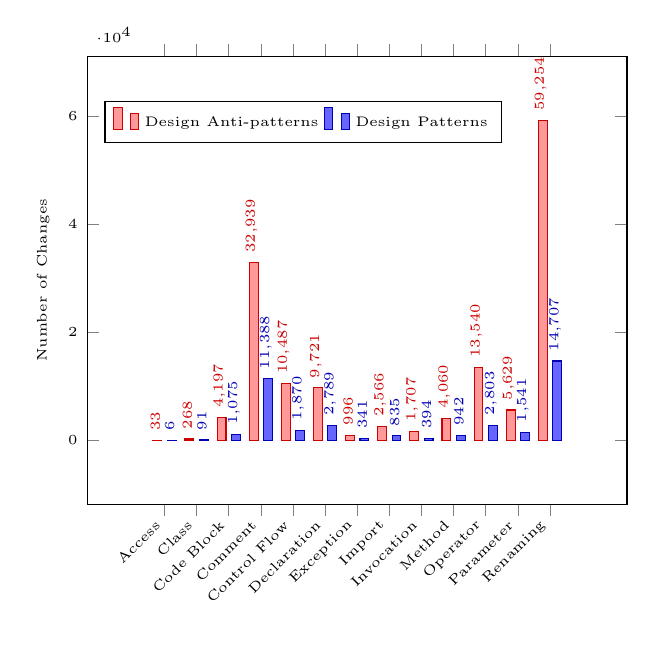
\begin{tikzpicture}
\pgfplotsset{every node/.append style={font=\tiny}}
\pgfplotsset{every tick label/.append style={font=\tiny}}
\begin{axis}[
    ybar,
    ymin=0,
    enlargelimits=0.2,
    legend style={at={(0.4,0.9)},anchor=north,legend columns=-1},
    bar width=1.12mm,
    ylabel={Number of Changes},
    symbolic x coords={Access, Class, Code Block, Comment, 
		Control Flow, Declaration, Exception, Import, Invocation, Method, Operator, Parameter, Renaming},
    xtick=data,
    x tick label style={rotate=45,anchor=east},
    nodes near coords,
    nodes near coords align={center},style={font=\tiny},
    every node near coord/.append style={rotate=90,anchor=south west,
    inner ysep=-1.75pt,}
    ]

\addplot [red!80!black,fill=red!40] coordinates {
(Access,33)
(Class,268) 
(Code Block,4197)
(Comment,32939)
(Control Flow,10487)
(Declaration,9721)
(Exception,996)
(Import,2566)
(Invocation,1707)
(Method,4060)
(Operator,13540)
(Parameter,5629)
(Renaming,59254)};
  
\addplot [blue!70!black,fill=blue!60] coordinates {
(Access,6) 
(Class,91)
(Code Block,1075) 
(Comment,11388)
(Control Flow,1870)
(Declaration,2789)
(Exception,341)
(Import,835)
(Invocation,394)
(Method,942)
(Operator,2803)
(Parameter,1541)
(Renaming,14707)};
\legend{Design Anti-patterns, Design Patterns}
\end{axis}
\end{tikzpicture}
}
\caption{Number of different types of changes in Eclipse classes with design anti-patterns and design patterns.}
\label{fig:FigureChangeEclipseNew}
\end{figure}

% Nuxeo
\begin{figure}
\centering
\scalebox{1.1}{
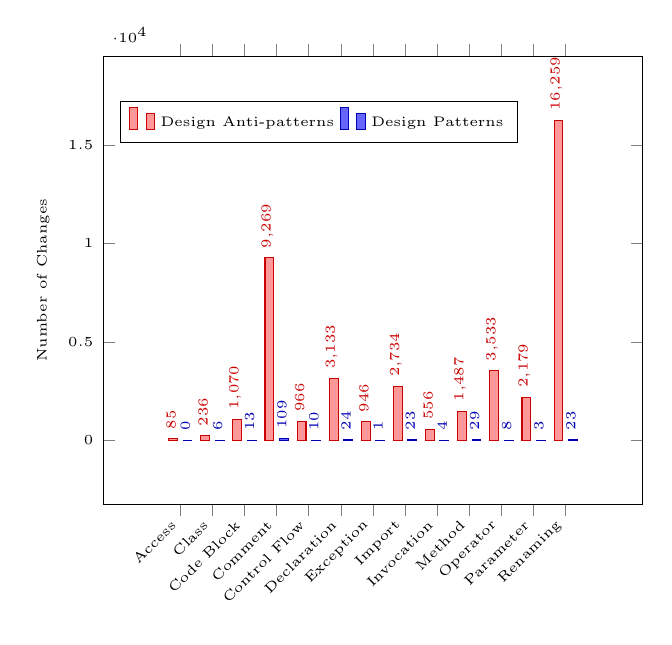
\begin{tikzpicture}
\pgfplotsset{every node/.append style={font=\tiny}}
\pgfplotsset{every tick label/.append style={font=\tiny}}
\begin{axis}[
    ybar,
    ymin=0,
    enlargelimits=0.2,
    legend style={at={(0.4,0.9)},anchor=north,legend columns=-1},
    bar width=1.12mm,
    ylabel={Number of Changes},
    symbolic x coords={Access, Class, Code Block, Comment, 
		Control Flow, Declaration, Exception, Import, Invocation, Method, Operator, Parameter, Renaming},
    xtick=data,
    x tick label style={rotate=45,anchor=east},
    nodes near coords,
    nodes near coords align={center},style={font=\tiny},
    every node near coord/.append style={rotate=90,anchor=south west,
    inner ysep=-1.75pt,}
    ]

\addplot [red!80!black,fill=red!40] coordinates {
(Access,85)
(Class,236) 
(Code Block,1070)
(Comment,9269)
(Control Flow,966)
(Declaration,3133)
(Exception,946)
(Import,2734)
(Invocation,556)
(Method,1487)
(Operator,3533)
(Parameter,2179)
(Renaming,16259)};
  
\addplot [blue!70!black,fill=blue!60] coordinates {
(Access,0) 
(Class,6)
(Code Block,13) 
(Comment,109)
(Control Flow,10)
(Declaration,24)
(Exception,1)
(Import,23)
(Invocation,4)
(Method,29)
(Operator,8)
(Parameter,3)
(Renaming,23)};
\legend{Design Anti-patterns, Design Patterns}
\end{axis}
\end{tikzpicture}
}
\caption{Number of different types of changes in Nuxeo classes with design anti-patterns and design patterns.}
\label{fig:FigureChangeNuxeoNew}
\end{figure}

% Ovirt
\begin{figure}
\centering
\scalebox{1.1}{
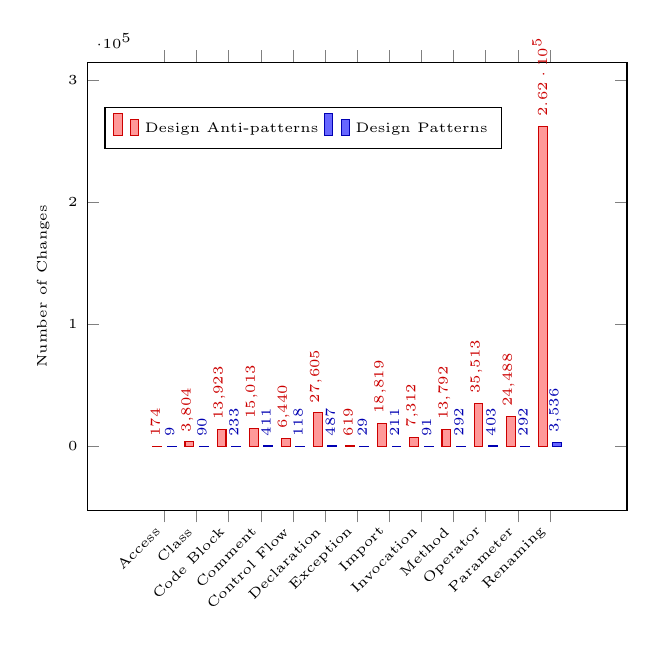
\begin{tikzpicture}
\pgfplotsset{every node/.append style={font=\tiny}}
\pgfplotsset{every tick label/.append style={font=\tiny}}
\begin{axis}[
    ybar,
    ymin=0,
    enlargelimits=0.2,
    legend style={at={(0.4,0.9)},anchor=north,legend columns=-1},
    bar width=1.12mm,
    ylabel={Number of Changes},
    symbolic x coords={Access, Class, Code Block, Comment, 
		Control Flow, Declaration, Exception, Import, Invocation, Method, Operator, Parameter, Renaming},
    xtick=data,
    x tick label style={rotate=45,anchor=east},
    nodes near coords,
    nodes near coords align={center},style={font=\tiny},
    every node near coord/.append style={rotate=90,anchor=south west,
    inner ysep=-1.75pt,}
    ]

\addplot [red!80!black,fill=red!40] coordinates {
(Access,174)
(Class,3804) 
(Code Block,13923)
(Comment,15013)
(Control Flow,6440)
(Declaration,27605)
(Exception,619)
(Import,18819)
(Invocation,7312)
(Method,13792)
(Operator,35513)
(Parameter,24488)
(Renaming,262491)};
  
\addplot [blue!70!black,fill=blue!60] coordinates {
(Access,9) 
(Class,90)
(Code Block,233) 
(Comment,411)
(Control Flow,118)
(Declaration,487)
(Exception,29)
(Import,211)
(Invocation,91)
(Method,292)
(Operator,403)
(Parameter,292)
(Renaming,3536)};
\legend{Design Anti-patterns, Design Patterns}
\end{axis}
\end{tikzpicture}
}
\caption{Number of different types of changes in oVirt classes with design anti-patterns and design patterns.}
\label{fig:FigureChangeoVirtNew}
\end{figure}

% Matsim
\begin{figure}
\centering
\scalebox{1.1}{
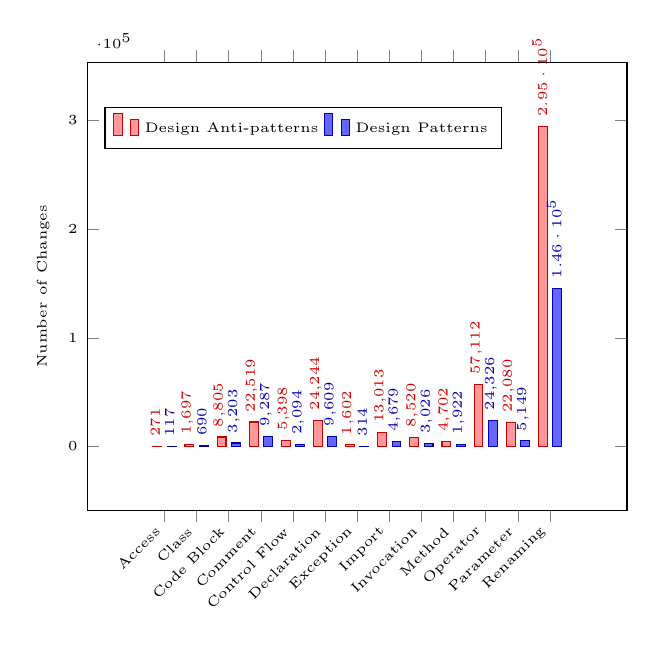
\begin{tikzpicture}
\pgfplotsset{every node/.append style={font=\tiny}}
\pgfplotsset{every tick label/.append style={font=\tiny}}
\begin{axis}[
    ybar,
    ymin=0,
    enlargelimits=0.2,
    legend style={at={(0.4,0.9)},anchor=north,legend columns=-1},
    bar width=1.12mm,
    ylabel={Number of Changes},
    symbolic x coords={Access, Class, Code Block, Comment, 
		Control Flow, Declaration, Exception, Import, Invocation, Method, Operator, Parameter, Renaming},
    xtick=data,
    x tick label style={rotate=45,anchor=east},
    nodes near coords,
    nodes near coords align={center},style={font=\tiny},
    every node near coord/.append style={rotate=90,anchor=south west,
    inner ysep=-1.75pt,}
    ]

\addplot [red!80!black,fill=red!40] coordinates {
(Access,271)
(Class,1697) 
(Code Block,8805)
(Comment,22519)
(Control Flow,5398)
(Declaration,24244)
(Exception,1602)
(Import,13013)
(Invocation,8520)
(Method,4702)
(Operator,57112)
(Parameter,22080)
(Renaming,294661)};
  
\addplot [blue!70!black,fill=blue!60] coordinates {
(Access,117) 
(Class,690)
(Code Block,3203) 
(Comment,9287)
(Control Flow,2094)
(Declaration,9609)
(Exception,314)
(Import,4679)
(Invocation,3026)
(Method,1922)
(Operator,24326)
(Parameter,5149)
(Renaming,145720)};
\legend{Design Anti-patterns, Design Patterns}
\end{axis}
\end{tikzpicture}
}
\caption{Number of different types of changes in Matsim classes with design anti-patterns and design patterns.}
\label{fig:FigureChangeMatsimNew}
\end{figure}

%ApacheIgnite
\begin{figure}
\centering
\scalebox{1.1}{
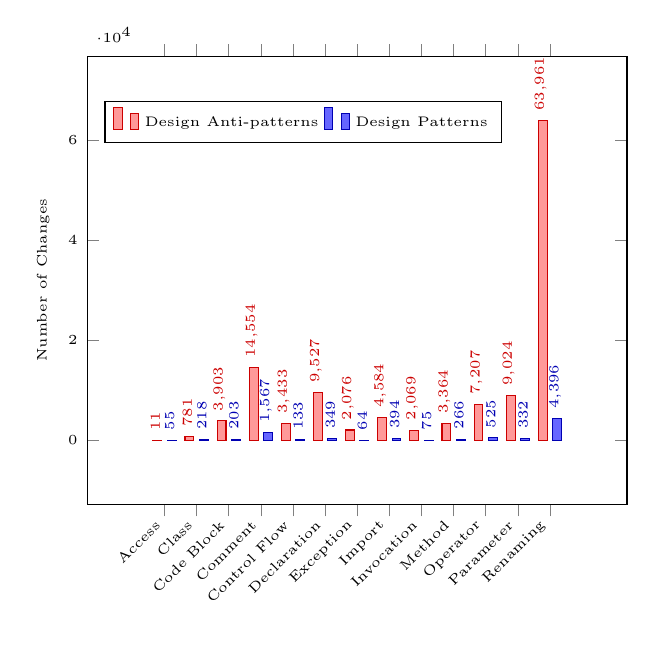
\begin{tikzpicture}
\pgfplotsset{every node/.append style={font=\tiny}}
\pgfplotsset{every tick label/.append style={font=\tiny}}
\begin{axis}[
    ybar,
    ymin=0,
    enlargelimits=0.2,
    legend style={at={(0.4,0.9)},anchor=north,legend columns=-1},
    bar width=1.12mm,
    ylabel={Number of Changes},
    symbolic x coords={Access, Class, Code Block, Comment, 
		Control Flow, Declaration, Exception, Import, Invocation, Method, Operator, Parameter, Renaming},
    xtick=data,
    x tick label style={rotate=45,anchor=east},
    nodes near coords,
    nodes near coords align={center},style={font=\tiny},
    every node near coord/.append style={rotate=90,anchor=south west,
    inner ysep=-1.75pt,}
    ]

\addplot [red!80!black,fill=red!40] coordinates {
(Access,11)
(Class,781) 
(Code Block,3903)
(Comment,14554)
(Control Flow,3433)
(Declaration,9527)
(Exception,2076)
(Import,4584)
(Invocation,2069)
(Method,3364)
(Operator,7207)
(Parameter,9024)
(Renaming,63961)};
  
\addplot [blue!70!black,fill=blue!60] coordinates {
(Access,55) 
(Class,218)
(Code Block,203) 
(Comment,1567)
(Control Flow,133)
(Declaration,349)
(Exception,64)
(Import,394)
(Invocation,75)
(Method,266)
(Operator,525)
(Parameter,332)
(Renaming,4396)};
\legend{Design Anti-patterns, Design Patterns}
\end{axis}
\end{tikzpicture}
}
\caption{Number of different types of changes in Apache Ignite classes with design anti-patterns and design patterns.}
\label{fig:FigureChangeApacheIgniteNew}
\end{figure}

%ApacheISolr
\begin{figure}
\centering
\scalebox{1.1}{
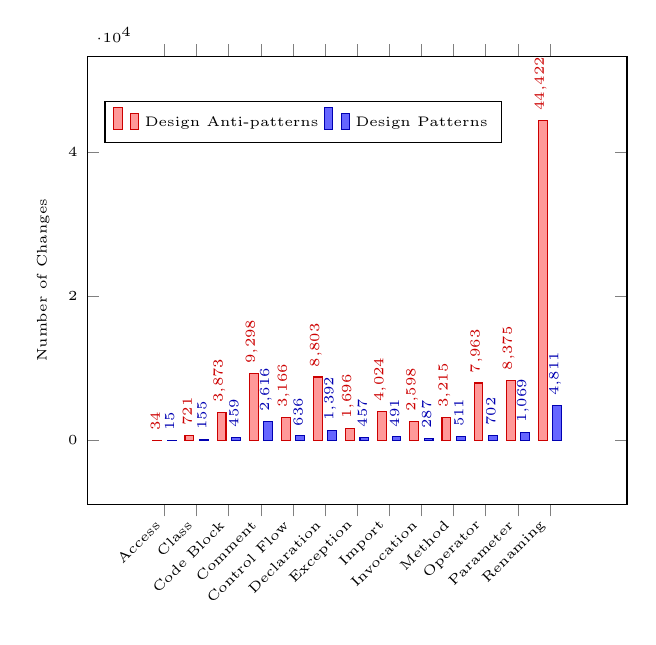
\begin{tikzpicture}
\pgfplotsset{every node/.append style={font=\tiny}}
\pgfplotsset{every tick label/.append style={font=\tiny}}
\begin{axis}[
    ybar,
    ymin=0,
    enlargelimits=0.2,
    legend style={at={(0.4,0.9)},anchor=north,legend columns=-1},
    bar width=1.12mm,
    ylabel={Number of Changes},
    symbolic x coords={Access, Class, Code Block, Comment, 
		Control Flow, Declaration, Exception, Import, Invocation, Method, Operator, Parameter, Renaming},
    xtick=data,
    x tick label style={rotate=45,anchor=east},
    nodes near coords,
    nodes near coords align={center},style={font=\tiny},
    every node near coord/.append style={rotate=90,anchor=south west,
    inner ysep=-1.75pt,}
    ]

\addplot [red!80!black,fill=red!40] coordinates {
(Access,34)
(Class,721) 
(Code Block,3873)
(Comment,9298)
(Control Flow,3166)
(Declaration,8803)
(Exception,1696)
(Import,4024)
(Invocation,2598)
(Method,3215)
(Operator,7963)
(Parameter,8375)
(Renaming,44422)};
  
\addplot [blue!70!black,fill=blue!60] coordinates {
(Access,15) 
(Class,155)
(Code Block,459) 
(Comment,2616)
(Control Flow,636)
(Declaration,1392)
(Exception,457)
(Import,491)
(Invocation,287)
(Method,511)
(Operator,702)
(Parameter,1069)
(Renaming,4811)};
\legend{Design Anti-patterns, Design Patterns}
\end{axis}
\end{tikzpicture}
}
\caption{Number of different types of changes in Apache Solr classes with design anti-patterns and design patterns.}
\label{fig:FigureChangeApacheSolrNew}
\end{figure}

% Mule
\begin{figure}
\centering
\scalebox{1.1}{
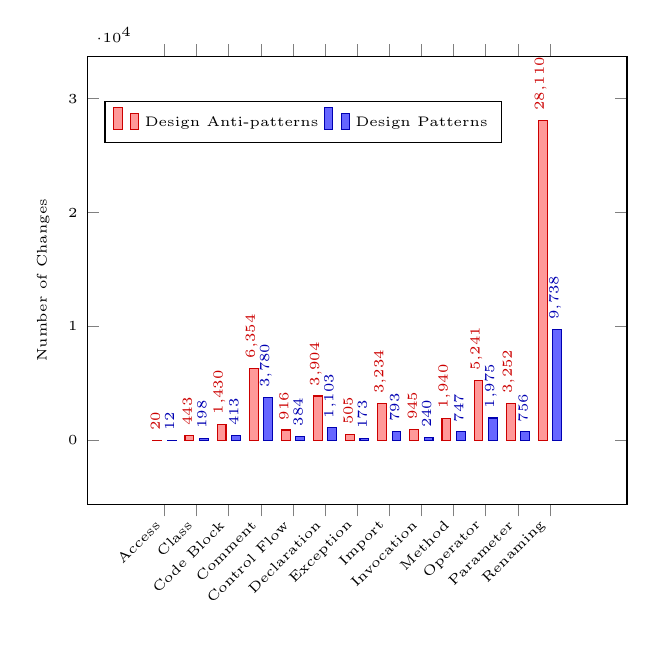
\begin{tikzpicture}
% \pgfplotsset{width = 10cm}
\pgfplotsset{every node/.append style={font=\tiny}}
\pgfplotsset{every tick label/.append style={font=\tiny}}
\begin{axis}[
    ybar,
    ymin=0,
    enlargelimits=0.2,
    legend style={at={(0.4,0.9)},anchor=north,legend columns=-1},
    bar width=1.12mm,
    ylabel={Number of Changes},
    symbolic x coords={Access, Class, Code Block, Comment, 
		Control Flow, Declaration, Exception, Import, Invocation, Method, Operator, Parameter, Renaming},
    xtick=data,
    x tick label style={rotate=45,anchor=east},
    nodes near coords,
    nodes near coords align={center},style={font=\tiny},
    every node near coord/.append style={rotate=90,anchor=south west,
    inner ysep=-1.75pt,}
    ]

\addplot [red!80!black,fill=red!40] coordinates {
(Access,20)
(Class,443) 
(Code Block,1430)
(Comment,6354)
(Control Flow,916)
(Declaration,3904)
(Exception,505)
(Import,3234)
(Invocation,945)
(Method,1940)
(Operator,5241)
(Parameter,3252)
(Renaming,28110)};
  
\addplot [blue!70!black,fill=blue!60] coordinates {
(Access,12) 
(Class,198)
(Code Block,413) 
(Comment,3780)
(Control Flow,384)
(Declaration,1103)
(Exception,173)
(Import,793)
(Invocation,240)
(Method,747)
(Operator,1975)
(Parameter,756)
(Renaming,9738)};
\legend{Design Anti-patterns, Design Patterns}
\end{axis}
\end{tikzpicture}
}
\caption{Number of different types of changes in Mule classes with design anti-patterns and design patterns.}
\label{fig:FigureChangeMuleNew}
\end{figure}

\paragraph{\textbf{Analysing change types of mutations}} During evolution, design patterns and design anti-patterns can mutate into other design patterns and design anti-patterns. We investigate which types of changes lead to such mutations. 
% The results of detected change types are contained in CSV files related to changed classes participating in design patterns and design anti-patterns for each system. Each CSV file includes the name of the two subsequent snapshots compared for change detection, the type of changes and the names of the classes changed. We compare two CSV files related to design patterns and design anti-patterns. By comparing the names of classes participating in occurrences of design patterns and design anti-patterns, we find the same class names which indicate that we have a mutation from design anti-patterns to design patterns and vice versa. 
Tables \ref{tab:dpapMutations} shows the number of each change types during the mutation for all the studied systems.

Results show that, in Apache Ignite, Renaming, Comment, and Declaration lead the most mutations from design anti-patterns (DAPs) to design patterns (DPs). It is almost the same for DPs-to-DAPs mutations but Parameter has more importance than Declaration. In Apache Solr and Eclipse for both DAPs-to-DPs and DPs-to-DAPs mutations, Renaming, Declaration, and Comment are the most representative change types. In Matsim, Renaming, Operator, and Declaration have the most impact on DAPs-to-DPs mutations while Renaming, Comment, and Operator lead to more DPs-to-DAPs mutations. In Mule, for both DAPs-to-DPs and DPs-to-DAPs mutations, Renaming, Comment, and Operator are the most representative change types. In Nuxeo, there are few mutations, in which Comment, Renaming, and Declaration yield DAPs-to-DPs mutations while Comment, Code Block, and Control Flow yield more DPs-to-DAPs mutations. Finally, in oVirt, Renaming, Declaration, and Comment are change types that lead to DAPs-to-DPs mutations while Renaming, Operator, and Declaration bring DPs-to-DAPs mutations.

Renaming is the most frequent change type. There are different types of renaming, described in \cite{arnaoudova2014repent}. In some types, an entity, \eg{} a package, a class, etc., is renamed. In other types, one or more terms are changed (simple and complex renaming). Sometimes, when one or more terms change, the meaning of the identifier also changes (semantic renaming). The grammar of an identifier may also change during evolution (grammar renaming). When developers use some tools to apply a renaming operation, the tool may not rename all variables consistently in all related files. Besides, certain source-code changes must be made together to preserve consistency. Changes in comments and declarations led to more mutations not as root causes of these mutations but because developers changed comments and declarations while evolving their systems for other reasons, \ie{} fixing faults. Future work include a manual, qualitative analysis of the mutations to identify their root causes.

\begin{tcolorbox}
\vspace{-0.1cm}
\textbf{Summary:} \emph{Some change types affect the mutations between design patterns and--or design anti-patterns more than others. We observe that the change types leading to mutations in all the studied systems are Renaming, Comment, Declaration, and Operator.}
\vspace{-0.1cm}
\end{tcolorbox}



\subsection{\textbf{RQ3:} \textit{\RQThree}}

\paragraph{\textbf{Motivation}} The results from RQ1 and RQ2 show that design patterns and design anti-patterns mutate during software evolution. However, they do not say anything about the impact of these mutations in software quality. Therefore, we investigate these mutations and their fault-proneness. Using this information, developers could understand the reasons of faults and take actions to reduce the risk of introducing faults.

\paragraph{\textbf{Analysing design patterns and design anti-patterns fault-proneness}} For each system, we mine its commit log and extract fault and commit IDs related to the faults and the dates when the faults were introduced. We look for faults introduced from one snapshot to the next. We use the dates to distinguish between faults appearing in one snapshot and those appearing between two extracted snapshots.

Table \ref{tab:DAP-DPfault} shows the numbers of faulty and clean of classes involved in patterns. One class can be involved in several faults in the studied snapshots so we show in Table \ref{tab:fault} the numbers of unique faulty and clean classes involved in patterns. Finally, in Table \ref{tab:faultpercentages}, we compare the percentages of faulty and clean classes involved in design patterns and design anti-patterns. Moreover, we show in Table \ref{tab:faultpercentages} the relative percentages of faults per class participating, or not, in design (anti-)patterns. 

With these tables, we summarise our whole dataset with: the numbers of (unique) faulty and non-faulty (clean) classes participating or not in design (anti-)patterns and their relative percentages. We thus can compare the prevalence of faults in different classes and confirm that classes participating in design anti-patterns have more faults than classes involved in design patterns. Thus, we have evidence supporting that classes that participate in design anti-patterns are more fault-prone than classes involved in design patterns.

For example, in Eclipse, 13.7\% of design pattern classes are fault-prone while 37.3\% of design anti-pattern classes are fault-prone. Table \ref{tab:faultpercentages} is showing similar trends in all the analysed systems.

\begin{table*} [ht]
\centering
\caption{Design anti-pattern and design-pattern mutations between faulty and clean classes}
\scalebox{0.8}{
\renewcommand{\arraystretch}{1.1}
\begin{tabular}{|l|r|r|r|}
\hline
\multirow{2}{*}{\textbf{\textbf{Systems}}} & \multicolumn{2}{c|}{\textbf{\# of Faulty classes}} & \multirow{2}{*}{\textbf{\# of Clean classes having DAPs, DPs}} \\
\cline{2-3}
 & Design Anti-patterns & Design Patterns & \\
 \hline \hline
 Apache Ignite & 10,984 & 1,051 & 81,093\\ 
 \hline
 Apache Solr & 11,156 & 219 & 109,225 \\
 \hline
 Eclipse & 15,240 & 5,182 & 19,928 \\
\hline
 Matsim & 4,053 & 1,888 & 896,510 \\
\hline
 Mule & 17,794 & 5,924 & 197,574 \\
\hline
 Nuxeo & 18,724 & 396 & 146,180 \\
\hline
 oVirt & 12,605 & 110 & 217,565 \\
\hline
\end{tabular}
}
\label{tab:DAP-DPfault}
\end{table*} 

\begin{table*} [ht]
\centering
\caption{Faulty and clean classes}
\scalebox{0.7}{
\renewcommand{\arraystretch}{1.1}
\begin{tabular}{|l|rr|rr|rr|rr|rr|}
\hline
\multirow{2}{*}{\textbf{Systems}} & \multicolumn{4}{c|}{\textbf{\# of Faulty Classes}} & \multicolumn{2}{c|}{\textbf{\# of Faulty Classes}} & \multicolumn{4}{c|}{\textbf{\# of Clean Classes}} \\
\cline{2-11}
& \multicolumn{2}{c|}{DAPs} & \multicolumn{2}{c|}{DPs} & \multicolumn{2}{c|}{\textbf{without Patterns}} & \multicolumn{2}{c|}{DAPs} &
\multicolumn{2}{c|}{DPs} \\
\hline \hline
Apache Ignite & 10,984 & (685) & 1,051 & (84) & 3,984 & (3,984) & 71,784 & (3,474) & 9,309 & (395)\\
\hline
Apache Solr & 11,156 & (638) & 219 & (22) & 6,351 & (6,351) & 101,044 & (3,447) & 8,181 & (392)\\
\hline
Eclipse & 15,240 & (591) & 5,182 & (217) & 12,285 & (12,285) & 13,610 & (562) & 6,318 & (213)\\
\hline
Matsim & 4,053 & (469) & 1,888 & (115) & 291 & (291) & 326,460 & (14,425) & 570,050 & (9,913)\\
\hline
Mule & 17,794 & (2,955) & 5,924 & (196) & 4,370 & (4,370) & 126,980 & (7,341) & 70,594 & (1,593)\\
\hline
Nuxeo & 18,724 & (1,487) & 396 & (68) & 7,414 & (7,414) & 143,276 & (3,659) & 2,904 & (170)\\
\hline
oVirt & 12,605 & (377) & 110 & (8) & 523 & (523) & 214,027 & (7,653) & 3,538 & (214)\\
\hline
\end{tabular}
}
\label{tab:fault}
\end{table*} 

\begin{table*} [ht]
\centering
\caption{Faulty and clean classes in percentages}
\scalebox{0.7}{
\renewcommand{\arraystretch}{1.1}
\begin{tabular}{|l|r|r|r|r|}
\hline
\multirow{2}{*}{\textbf{Systems}} & \multicolumn{2}{c|}{\textbf{Design anti-patterns}} & \multicolumn{2}{c|}{\textbf{Design patterns}} \\
\cline{2-5}
& Faulty Classes (\%) & Clean Classes (\%) &
Faulty Classes (\%) & Clean Classes (\%) \\
\hline \hline
Apache Ignite & 14.7\% & 74.9\% & 1.8\% & 8.5\% \\
\hline
Apache Solr & 14.1\% & 76.6\% & 0.48\% & 8.7\% \\
\hline
Eclipse & 37.3\% & 35.5\% & 13.7\% & 13.4\% \\
\hline
Matsim & 1.9\% & 57.9\% & 0.46\% & 39.7\% \\
\hline
Mule & 24.4\% & 60.7\% & 1.6\% & 13.2\% \\
\hline
Nuxeo & 27.6\% & 67.9\% & 1.3\% & 3.2\%\\
\hline
oVirt & 4.6\% & 92.7\% & 0.09\% & 2.6\%\\
\hline
\end{tabular}
}
\label{tab:faultpercentages}
\end{table*} 



\paragraph{\textbf{Analyzing mutations fault-proneness}} A mutation between design patterns and design anti-patterns can lead to faults. We use clean and faulty classes and their participation (or not) into design patterns and design anti-patterns to identify the mutations experienced by these faulty classes.

Table \ref{tab:TransFault} presents the most representative mutations that led to faults in each studied system. We observe that mutations from design anti-patterns to other design anti-patterns are more faulty. LongParameterList to LongMethod or LongMethod to LazyClass are such mutations in Apache Ignite. 

In Eclipse, Matsim, and Mule, there are mutations from design patterns to design patterns that also led to more faults. FactoryMethod to Decorator in Eclipse, Builder to FactoryMethod in Matsim and Mule are such mutations. 

There are also mutations from design anti-patterns to design patterns that led to faults as well, like AntiSingleton to FactoryMethod in Matsim or FactoryMethod to LongMethod in Eclipse. 

% Design anti-patterns are introduced by ``bad” implementations or design choices and such choices are implementing or designing a (or part of a) class. This could make the classes very large and complex leading to comprehension overheads to the developers. On the other hand, design patterns are good solutions to solve the design and implementation problems in the classes. Thus, the classes containing design anti-patterns are likely to be more fault-prone than classes containing design patterns; which is supported by our findings.

\begin{table*} [ht]
\centering
\caption{Most representative mutations between design patterns and design anti-patterns according to their mutation probabilities and fault-proneness}

\scalebox{0.8}{
\renewcommand {\arraystretch} {1.1}
\begin{tabular}{|l|l|l|l|r|}
\hline
\textbf{System} & \textbf{Mutation Type} & \textbf{From}  & \textbf{To} & \textbf{Probability} \\ \hline
\hline
\multirow{2}{*}{Apache Ignite} & 
 DAP$\,\to\,$DAP & LongParameterList & LongMethod & 0.571\\
\cline{2-5}
& DAP$\,\to\,$DAP & LongMethod & LazyClass & 0.285\\
\cline{2-5}
\hline
\multirow{3}{*}{Apache Solr} &  DAP$\,\to\,$DAP & RefusedParentBequest & MessageChain & 0.427\\
\cline{2-5}
& DAP$\,\to\,$DAP & LongMethod & LazyClass & 0.156 \\
\cline{2-5}
& DAP$\,\to\,$DAP & ComplexClass & ClassDataShouldBePrivate & 0.156\\
\cline{2-5}
\hline 
\multirow{3}{*}{Eclipe IDE} &  
 DP$\,\to\,$DP & FactoryMethod & Decorator & 0.492\\
 \cline{2-5} 
  & DAP$\,\to\,$DAP & LongMethod & LazyClass & 0.385\\
\cline{2-5}
 & DP$\,\to\,$DAP & FactoryMethod & LongMethod & 0.056\\
\cline{2-5}
\hline 
\multirow{3}{*}{Matsim} & 
DP$\,\to\,$DP & Builder & FactoryMethod & 0.677\\
\cline{2-5}
& DAP$\,\to\,$DAP & SpagettiCode & RefusedParentBequest & 0.152\\
\cline{2-5}
 & DAP$\,\to\,$DP & AntiSingleton & FactoryMethod & 0.114\\
\cline{2-5}
\hline 
\multirow{3}{*}{Mule} & 
DP$\,\to\,$DP & Builder & FactoryMethod & 0.479 \\
\cline{2-5}
& DAP$\,\to\,$DP & ComplexClass & FactoryMethod & 0.264\\
\cline{2-5}
& DAP$\,\to\,$DAP & ComplexClass & ClassDataShouldBePrivate & 0.223\\ 
\cline{2-5}
\hline  
\multirow{2}{*}{Nuxeo} & DAP$\,\to\,$DAP & LazyClass & LargeClass & 0.285\\
\cline{2-5}
 & DP$\,\to\,$DP & Singleton & FactoryMethod & 0.495\\
\hline 
\multirow{2}{*}{oVirt} & DAP$\,\to\,$DAP & Blob & AntiSingleton & 0.722\\ 
\cline{2-5}
 & DP$\,\to\,$DP & Singleton & Prototype& 0.166\\ 
\hline 
\end{tabular}
}
\label{tab:TransFault}
\end{table*} 

\begin{tcolorbox}
\vspace{-0.1cm}
\textbf{Summary:} \emph{We observed that in some systems, as expected and shown in previous work, design anti-patterns are more fault-prone than design patterns. We also showed that some mutations are more fault-prone than others, in particular mutations from design anti-patterns to design patterns or to other design anti-patterns.}
\vspace{-0.1cm}
\end{tcolorbox}



\subsection{\textbf{RQ4:} \textit{\RQFour}}

\paragraph{\textbf{Motivation}} Different types of changes have different impacts on the software systems due to their differences in functionality and the ripple effects of changes. Some types of changes likely introduce more faults than others. Thus, understanding which types of changes increase the fault-proneness of the mutations could help developers to foresee and prevent faults by preventing/planning such changes during software evolution.

\paragraph{\textbf{Analysing change types leading to faults}} We use the same data as in RQ2 and RQ3. For each system, we identify the number of faulty classes that have changed through mutations between design anti-patterns and--or design patterns. Table \ref{tab:ChangeAn2De} shows the number of change types that led to faults. We report that, in all studied systems, Renaming, Comment, and Operator are the change types that lead to more faults.

\begin{table*}[ht]
\centering
\caption{Numbers of change types in the studied systems leading to faults} \label{tab:noFaultyChanges}
\scalebox{0.71}{
\renewcommand{\arraystretch}{1.1}
\begin{tabular}{|p{2.1cm}|r|r|r|r|r|r|r|}\hline
\textbf{Systems $\rightarrow$ }& \textbf{Apache Ignite} & \textbf{Apache Solr} & \textbf{Eclipse~~~} & \textbf{Matsim~~~} & \textbf{Mule~~~} & \textbf{Nuxeo~~~} & \textbf{oVirt~~~}\\\hline
\textbf{\textbf{Change Types}} &\# changes  &\# changes&\# changes &\# changes & \# changes &\# changes &\# changes\\
\hline \hline
  Access &18  &18  & 37 & 22 & 11 & 62 & 25\\ \hline
  Class &689  &431  &306  &306  & 422 &208  &763 \\ \hline
  Code block & 2,972 & 2,102 & 4,919 & 1,284 &1,306  & 854 & 3,833\\ \hline
  Comment & 12,169 & 5,498 & 38,150 & 2,813 & 6,270 &6,161  &4,653 \\ \hline
  Control flow &2,903  & 1,935 & 11,678 & 660 &  1067& 819 &2,406 \\ \hline
  Declaration &5,912  &  5,386& 11651 &  3,129& 3,191 & 2,628 &7,484 \\ \hline
  Exception &1,696  & 1221 & 1255 & 140 &  526& 786&  210\\ \hline
  Import & 2,831 &2,400  &2,958  & 1,425 &2,443  & 2,064 & 4,268 \\ \hline
  Invocation &1,550  &1,196  & 1,986 & 1,061 & 840 & 476 &1,882 \\ \hline
  Method & 2,509 & 1,851 & 4,093 &637  & 1,697 & 1,229 & 3,619\\ \hline
  Operator &5,120  & 4,364 & 16,094 & 6,215 & 4,228 & 2,675 & 8,134\\ \hline
  Parameter & 6,418 & 3,504 & 5,108 & 2,655 & 2,607 & 1,815 & 5,337 \\ \hline
  Renaming & 47,811 & 24,640 & 67,040 & 32,445 & 22,968 &  12,736& 65,245 \\ \hline
  \textbf{Total changed classes} &  5,505& 4,163 & 11,934 & 3,073 & 4,324 & 3,514 &7,150 \\ \hline
\end{tabular}
}
\label{tab:ChangeAn2De}
\end{table*} 

\paragraph{\textbf{Analyzing fault-proneness of classes with design patterns and design anti-patterns}} Table \ref{tab:Changefault} presents the numbers of faulty changed classes and Figures \ref{fig:DPFaultyChangedClasses} and \ref{fig:APFaultyChangedClasses} show the percentages of faulty changed classes participating in design patterns and design anti-patterns for all the systems. Figure \ref{fig:AP_DPFaultyChangedClasses} compares the numbers of faulty and clean classes changed in all the snapshots of the studied systems. Each first bar presents the number of faulty and clean changed classes participating in design anti-patterns and the second one is faulty and clean classes having design patterns. We observe that change types have impacts on the fault-proneness of changed classes. Changed classes participating in design patterns are less faulty than those participating only in design anti-patterns. 

Figures \ref{fig:DPFaultyChangedClasses} and \ref{fig:APFaultyChangedClasses} show that some of the faulty classes are those which had changed in the past. For example, in Eclipse, the percentages of faulty classes participating in design patterns is 81\% while for those participating in design anti-patterns it is 86\%. The differences between these two categories are more visible in Apache Solr, where 51\% of changed classes are participating in design anti-patterns, and only 11\% of them have design patterns. In Rhino, changes impact fault-proneness significantly, because, on average, more than 85\% of changed classes are faulty. Thus, the trend is that changed classes with design anti-patterns tend to be more fault-prone than changed classes with design patterns.

\begin{table*} [ht]
\centering
\caption{Numbers of faulty and clean changed classes}
\scalebox{0.9}{
\renewcommand{\arraystretch}{1.1}
\begin{tabular}{|l|l|r|r|}
\hline
\textbf{Systems} & \textbf{Patterns}  & \textbf{\# Faulty classes} & \textbf{\# Clean classes}\\
\hline \hline
\multirow{2}{*}{Apache Ignite} & Design Anti-patterns & 5,112 & 4,178\\ 
 \cline{2-4}
 & Design Patterns & 393 & 464\\
\hline
\multirow{2}{*}{Apache Solr} & Design Anti-patterns & 4,035 & 3,921\\
\cline{2-4}
 & Design patterns & 128 & 1,064\\
\hline
\multirow{2}{*}{Eclipse} & Design Anti-patterns & 9,406 & 1,551\\
\cline{2-4}
 & Design patterns & 2,554 & 601\\
\hline
\multirow{2}{*}{Matsim} & Design Anti-patterns & 2,549 & 30,042\\
\cline{2-4}
 & Design patterns & 524 & 13,244\\
\hline
\multirow{2}{*}{Mule} & Design Anti-patterns & 3,374 & 2,311\\
\cline{2-4}
 & Design patterns & 950 & 1,225\\
\hline
\multirow{2}{*}{Nuxeo} & Design Anti-patterns & 3,469 & 1,935\\
\cline{2-4}
 & Design patterns & 45 & 36\\
\hline
\multirow{2}{*}{oVirt} & Design Anti-patterns & 7,075 & 27,705\\
\cline{2-4}
 & Design patterns & 75 & 482\\
\hline
\end{tabular}
}
\label{tab:Changefault}
\end{table*} 


\begin{figure}[ht]
\centering
\scalebox{0.8}{
  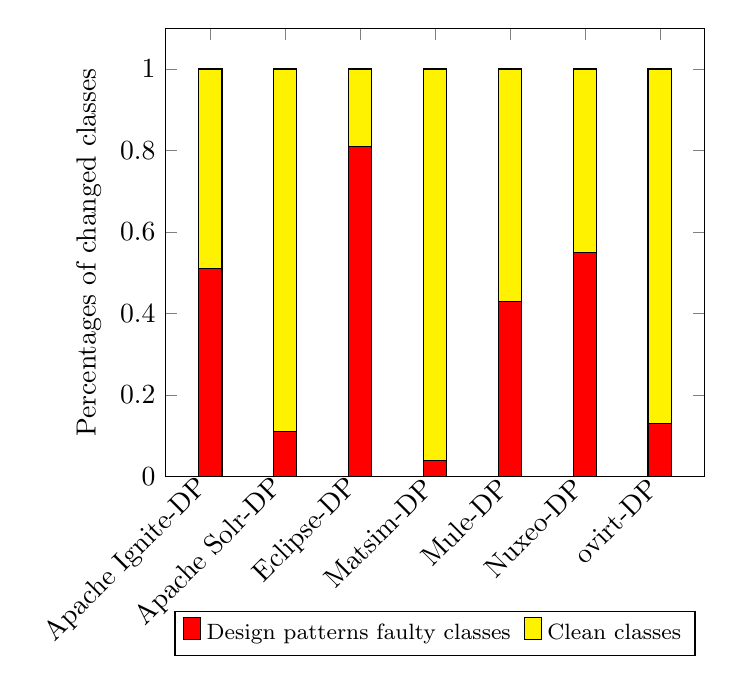
\begin{tikzpicture}
  \begin{axis}[
      every node near coord/.style={
     },
     legend style={
       font=\footnotesize,
       cells={anchor=east},
       legend columns=5,
       at={(0.50,-0.30)},
       anchor=north,
       /tikz/every even column/.append style={column sep=0.1cm}
     },
    title={},
    ybar stacked, ymin=0,
    bar width=3mm,
    ylabel={Percentages of changed classes},
    symbolic x coords=     {Apache Ignite-DP, Apache Solr-DP, Eclipse-DP, Matsim-DP, Mule-DP, Nuxeo-DP, ovirt-DP},
    xtick=data,
    x tick label style={rotate=45,anchor=east},
]
  %F
  \addplot [fill=red] coordinates {
%  ({Apache Ignite-AP},0.55)
  ({Apache Ignite-DP},0.51)
%  ({Apache Solr-AP},0.51)
  ({Apache Solr-DP},0.11)
%  ({Eclipse-AP},0.86)
  ({Eclipse-DP},0.81)
%  ({Matsim-AP},0.08)
  ({Matsim-DP},0.04)
%  ({Mule-AP},0.59)
  ({Mule-DP},0.43)
%  ({Nuxeo-AP},0.64)
  ({Nuxeo-DP},0.55)
%  ({Ovirt-AP},0.20)
  ({ovirt-DP},0.13)
};
    \addplot [fill=yellow] coordinates {
%  ({Apache Ignite-AP},0.45)
  ({Apache Ignite-DP},0.49)
%  ({Apache Solr-AP},0.49)
  ({Apache Solr-DP},0.89)
%  ({Eclipse-AP},0.14)
  ({Eclipse-DP},0.19)
%  ({Matsim-AP},0.92)
  ({Matsim-DP},0.96)
%  ({Mule-AP},0.41)
  ({Mule-DP},0.57)
%  ({Nuxeo-AP},0.36)
  ({Nuxeo-DP},0.45)
%  ({Ovirt-AP},0.80)
  ({ovirt-DP},0.87)
};
  \legend {Design patterns faulty classes, Clean classes} 
  \end{axis}
  \end{tikzpicture}
  }
 \caption{Faulty changed classes percentages with design pattern in the studied systems} 
\label{fig:DPFaultyChangedClasses}
\end{figure}

\begin{figure}[ht]
\centering
\scalebox{0.8}{
  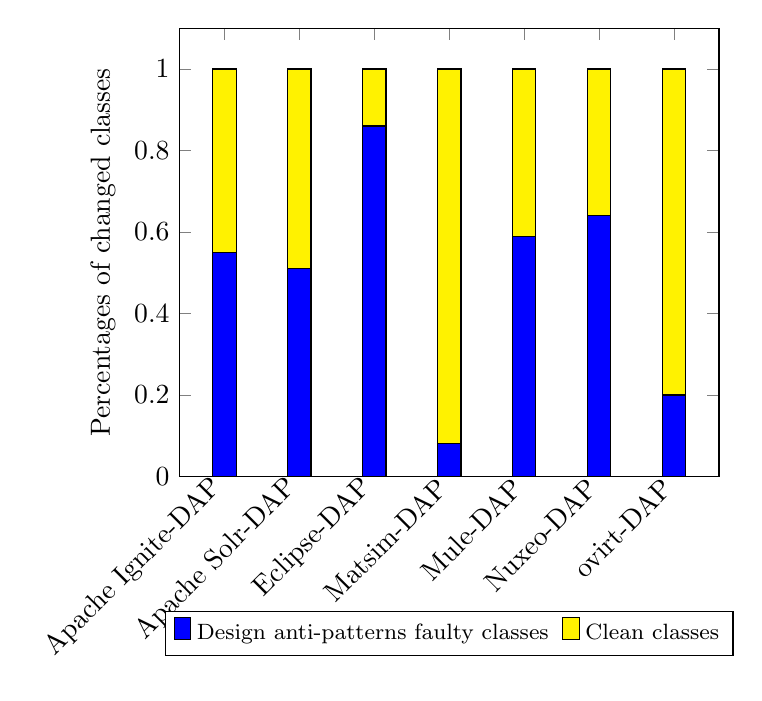
\begin{tikzpicture}
  \begin{axis}[
      every node near coord/.style={
     },
     legend style={
       font=\footnotesize,
       cells={anchor=east},
       legend columns=5,
       at={(0.50,-0.30)},
       anchor=north,
       /tikz/every even column/.append style={column sep=0.1cm}
     },
    title={},
    ybar stacked, ymin=0,
    bar width=3mm,
    ylabel={Percentages of changed classes},
    symbolic x coords=     {Apache Ignite-DAP, Apache Solr-DAP, Eclipse-DAP, Matsim-DAP, Mule-DAP, Nuxeo-DAP, ovirt-DAP},
    xtick=data,
    x tick label style={rotate=45,anchor=east},
]
  %F
  \addplot [fill=blue] coordinates {
  ({Apache Ignite-DAP},0.55)
%  ({Apache Ignite-DP},0.51)
  ({Apache Solr-DAP},0.51)
%  ({Apache Solr-DP},0.11)
  ({Eclipse-DAP},0.86)
%  ({Eclipse-DP},0.81)
  ({Matsim-DAP},0.08)
%  ({Matsim-DP},0.04)
  ({Mule-DAP},0.59)
%  ({Mule-DP},0.43)
  ({Nuxeo-DAP},0.64)
%  ({Nuxeo-DP},0.55)
  ({ovirt-DAP},0.20)
%  ({Ovirt-DP},0.13)
};

  \addplot [fill=yellow] coordinates {
  ({Apache Ignite-DAP},0.45)
%  ({Apache Ignite-DP},0.49)
  ({Apache Solr-DAP},0.49)
%  ({Apache Solr-DP},0.89)
  ({Eclipse-DAP},0.14)
%  ({Eclipse-DP},0.19)
  ({Matsim-DAP},0.92)
%  ({Matsim-DP},0.96)
  ({Mule-DAP},0.41)
%  ({Mule-DP},0.57)
  ({Nuxeo-DAP},0.36)
%  ({Nuxeo-DP},0.45)
  ({ovirt-DAP},0.80)
%  ({Ovirt-DP},0.87)
};
  \legend {Design anti-patterns faulty classes, Clean classes} 
  \end{axis}
  \end{tikzpicture}
  }
 \caption{Faulty changed classes with design anti-patterns percentages in the studied systems} 
\label{fig:APFaultyChangedClasses}
\end{figure}

\begin{figure}
\centering
\scalebox{1.1}{
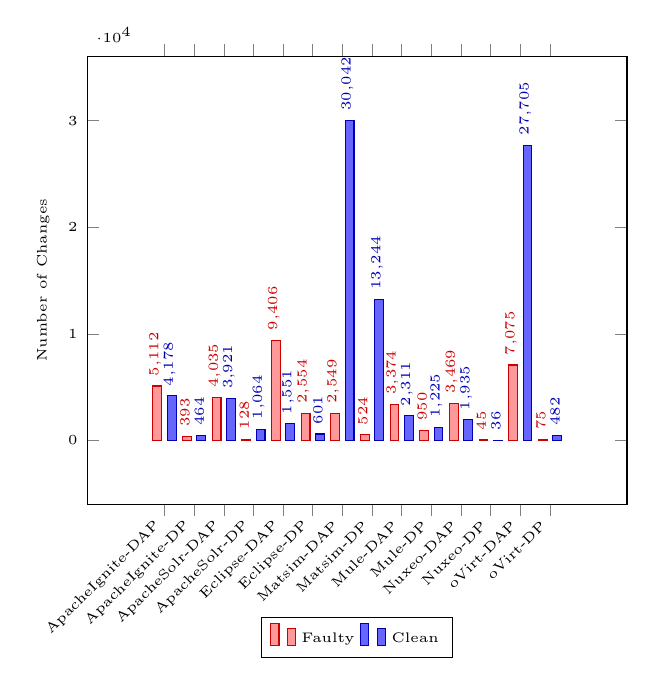
\begin{tikzpicture}
\pgfplotsset{every node/.append style={font=\tiny}}
\pgfplotsset{every tick label/.append style={font=\tiny}}
\begin{axis}[
    ybar,
    ymin=0,
    enlargelimits=0.2,
    legend style={at={(0.5,-0.25)},anchor=north,legend columns=-1},
    bar width=1.12mm,
    ylabel={Number of Changes},
    symbolic x coords={ApacheIgnite-DAP, ApacheIgnite-DP, ApacheSolr-DAP, ApacheSolr-DP, Eclipse-DAP, Eclipse-DP, Matsim-DAP, Matsim-DP, Mule-DAP, Mule-DP, Nuxeo-DAP, Nuxeo-DP, oVirt-DAP, oVirt-DP},
    xtick=data,
    x tick label style={rotate=45,anchor=east},
    nodes near coords,
    nodes near coords align={center},style={font=\tiny},
    every node near coord/.append style={rotate=90,anchor=south west,
    inner ysep=-1.75pt,}
    ]

\addplot [red!80!black,fill=red!40] coordinates {
(ApacheIgnite-DAP,5112) (ApacheIgnite-DP,393) (ApacheSolr-DAP,4035) (ApacheSolr-DP,128) (Eclipse-DAP,9406) (Eclipse-DP,2554) (Matsim-DAP,2549) (Matsim-DP,524) (Mule-DAP,3374) (Mule-DP,950) (Nuxeo-DAP,3469) (Nuxeo-DP,45) (oVirt-DAP,7075) (oVirt-DP,75)};
  
\addplot [blue!70!black,fill=blue!60] coordinates {
(ApacheIgnite-DAP,4178) (ApacheIgnite-DP,464) (ApacheSolr-DAP,3921) (ApacheSolr-DP,1064) (Eclipse-DAP,1551) (Eclipse-DP,601) (Matsim-DAP,30042) (Matsim-DP,13244) (Mule-DAP, 2311) (Mule-DP,1225) (Nuxeo-DAP,1935) (Nuxeo-DP,36) (oVirt-DAP,27705) (oVirt-DP,482)};
\legend{Faulty, Clean}
\end{axis}
\end{tikzpicture}
}
\caption{Faulty changed classes with design anti-patterns and design patterns in the studied systems} 
\label{fig:AP_DPFaultyChangedClasses}
\end{figure}

\begin{tcolorbox}
\vspace{-0.1cm}
\textbf{Summary:} \emph{Some change types applied to design patterns and design anti-patterns make software systems more fault-prone compared to others. We observed that, in all the studied systems, Renaming, Comment, and Operator are the change types from design patterns to design anti-patterns that most lead to faults.}
\vspace{-0.1cm}
\end{tcolorbox}
To put our results in a broader context, let us briefly discuss alternative methods for 
classical simulation of quantum circuits. Vector-based simulators~\cite{de2007massively,smelyanskiy2016qhipster,haner20170}
represent $n$-qubit quantum states by complex vectors of size $2^n$
stored in a classical memory.
The state vector is updated
upon application of each gate by performing sparse
matrix-vector multiplication. The memory footprint limits 
the method to small number of qubits. For example, 
H{\"a}ner and Steiger~\cite{haner20170}
reported a simulation of
quantum circuits with $n=45$ qubits and a few hundred gates 
using a  supercomputer with $0.5$ petabytes of memory.
In certain special cases 
the memory footprint can be reduced 
by recasting the simulation problem as a 
tensor network contraction~\cite{markov2008simulating,boixo2017simulation,aaronson2016complexity}.
Several tensor-based simulators have been developed~\cite{pednault2017breaking,li2018quantum,chen2018classical} 
for geometrically local  shallow quantum  circuits that include only nearest-neighbor
gates on a 2D grid of qubits~\cite{boixo2018characterizing}.
These methods enabled simulations of systems with more than $100$ qubits~\cite{chen2018classical}.
However, it is expected~\cite{alibaba} that for general (geometrically non-local) circuits 
of size $poly(n)$  the runtime of tensor-based simulators scales as $2^{n-o(n)}$.

In contrast, Clifford simulators described in the present paper are applicable to large-scale circuits
without any locality properties as long as the circuit is dominated by Clifford gates. 
This regime may be important for verification of first fault-tolerant quantum circuits
where  logical non-Clifford gates are expected to be scarce due to their high implementation
cost~\cite{fowler2013surface,jones2013low}.
Another advantage of Clifford simulators is their ability to sample the output
distribution of the circuit (as opposed to computing individual output amplitudes).
This is more close to what one would expect from the actual quantum computer. 
For example, a single run of the heuristic sum-over-Cliffords simulator
described in Section~\ref{heuristic} produces thousands of samples from the (approximate) output distribution. 
In contrast, a single run of a tensor-based simulator typically computes a single amplitude of the
output state.  Thus we believe that our techniques 
extend the reach of classical simulation algorithms complementing
the existing vector- or tensor-based simulators.

%PC:
A version of the sum-over-Cliffords simulator using the Metropolis sampling method is also publicly available
as part of \texttt{Qiskit-Aer}, the classical simulation framework of IBM's quantum
programming suite \texttt{Qiskit}~\cite{Qiskit}. This enables classical simulation and verification of quantum
circuits built in Qiskit on system sizes above $30$ qubits, which quickly become inaccessible with the
default vector-based method. This version also supports parallel processing over the stabilizer state decomposition,
which improves the performance of the Metropolis step.

%SBB:
Let us briefly comment on how simulators based on the stabilizer rank compare
with quasi-probability  methods~\cite{pashayan15,Delfosse15rebits,kocia2017discrete}.
The latter use a discrete Wigner function representation of quantum states
and Monte Carlo sampling
to approximate a given output probability of the target circuit with a small
additive error. Negativity of the Wigner function is an important parameter
that quantifies severity of the ``sign problem" associated with the Monte Carlo sampling.
The negativity also controls the runtime of quasi-probability methods. 
For example, the simulator proposed in~\cite{pashayan15}
has runtime $\epsilon^{-2} M^2$, where $M$ is the negativity and $\epsilon$
is the desired approximation error. In contrast to stabilizer rank simulators,
quasi-probability methods do not directly apply to stabilizer
operations on qubits since the latter are not known to have a non-negative Wigner function 
representation~\cite{Delfosse15rebits,karanjai2018contextuality}.
Furthermore, such methods are not well-suited for sampling the output
distribution since this task requires a small {\em multiplicative} error in 
approximating individual output probabilities. 

Our work leaves several  open questions. 
Since the efficiency of Clifford simulators hinges on the ability to find low-rank
stabilizer decompositions of multi-qubit magic states, 
improved techniques for finding such decompositions are of great interest. 
For example, consider a magic state $|\psi\ra=U|+\ra^{\otimes n}$, where 
$U$ is a diagonal circuit composed of $Z,CZ$, and $CCZ$ gates.
We anticipate that a low-rank exact stabilizer decomposition of $\psi$ can be 
found by computing the {\em transversal number}~\cite{alon1990transversal} of a suitable hypergraph describing
the placement of CCZ gates. Such low-rank decompositions may lead to more efficient
simulation algorithms for Clifford+CCZ circuits. We leave as an open question whether
the stabilizer extent $\xi(\psi)$ is multiplicative under tensor products for general states $\psi$.
Finally, it is of great interest to derive lower bounds on the stabilizer rank
of $n$-qubit magic states scaling exponentially with $n$. 






\section{Threats to Validity}
\label{sec:Treats to Validity}

We now discuss potential threats to the validity of the results of our study, following existing guidelines \cite{yin2013case,wohlin2012experimentation}.


\paragraph{Construct validity} These threats concern the relation between theory and observation. We know that the used design pattern and design anti-pattern detection techniques (DECOR and DeMIMA) in this study include some subjective understanding related to the definition of design patterns and design anti-patterns. Their authors reported recall rates of 100$\%$ for both techniques while the precision in the worst case was 31$\%$. We accept that the precision of these techniques is a concern. Some false positive classes may pass the validation because they ``looks like'' playing a role in some patterns.

We also accept that, in finding change types which led to faults, we could have matched classes that are not representing the actual same class. For example, class \texttt{C} is not match with \texttt{a.b.C.java} but could be matched with the \texttt{b.c.java}. Moreover, we know that during evolution, class names change as well. As for precision, the manual validation could be affected by subjectiveness or human error.  We should consider each type of renaming as we may misinterpret that there is a mutation between design patterns and design anti-patterns, while in fact the class name changed and the patterns remained stable. 



\paragraph{Internal validity} This threat concerns factors affecting our results. This threat is about the causality drawn from the study. It concerns our selection of studied systems and methodology. The accuracy of DECOR and DeMIMA impacts our results, because the number of design patterns and design anti-patterns computed with DECOR and DeMIMA is used to calculate the probabilities of mutations. Other detection techniques should be used to validate our findings.

Our results show correlations between design anti-patterns and design patterns, their mutations, and faults. However, they do not show causation. Hence, it is possible that some of the changes, which led to mutations, \eg{} changes to comments, although correlated to mutations, are not the root causes of these mutations. Identifying these root causes would require studying each change leading to mutations individually, manually, which is future work.



\paragraph{Conclusion validity} These threats concern the relationship between the treatment and the results. We paid attention in choosing the systems.

We used the SZZ algorithm \cite{sliwerski2005changes} to identify commits introducing faults. Although this algorithm may yield false positive results, it has been successfully employed in previous works, such as \cite{kamei2013large,fukushima2014empirical}. In this paper, to increase the algorithm's accuracy, we removed all fault-inducing commit candidates that only changed blank or comment lines. Moreover, the static analysis tool, srcML, can identify about 100 types of code elements from source code.

To make our results more actionable for software practitioners, we manually grouped similar element tags into 12 major change types as shown in Table~\ref{tab:Change_types}, which can help developers carefully change and review fault-prone code.



\paragraph{Reliability Validity} These threats concern the possibility of replicating the study. We provide all the necessary data on-line\footnote{\url{http://www.ptidej.net/downloads/replications/emse19c/}} to help other researchers replicate our work.



\paragraph{External validity} These threats concern the ability to generalize our results. We studied seven software systems with different sizes, domains, and complexity. We selected only Java systems because of the tools. We also chose some of these systems because they have been used in previous studies. Their numbers of lines of code range from hundred of thousands to several millions. These systems are widely used and have active developers community. They have several years of evolution histories. They are available on-line. However, all of them are written in Java and are open source. In the future, we plan to investigate more diverse set of systems. Moreover, we also want to study larger projects, with other programming languages, such as C++. 

We analysed commits instead of releases to cover as much as possible the whole histories of these systems. We choose thirteen design anti-patterns and eight design patterns among the many available patterns.
\section{Conclusion}
We have presented a neural performance rendering system to generate high-quality geometry and photo-realistic textures of human-object interaction activities in novel views using sparse RGB cameras only. 
%
Our layer-wise scene decoupling strategy enables explicit disentanglement of human and object for robust reconstruction and photo-realistic rendering under challenging occlusion caused by interactions. 
%
Specifically, the proposed implicit human-object capture scheme with occlusion-aware human implicit regression and human-aware object tracking enables consistent 4D human-object dynamic geometry reconstruction.
%
Additionally, our layer-wise human-object rendering scheme encodes the occlusion information and human motion priors to provide high-resolution and photo-realistic texture results of interaction activities in the novel views.
%
Extensive experimental results demonstrate the effectiveness of our approach for compelling performance capture and rendering in various challenging scenarios with human-object interactions under the sparse setting.
%
We believe that it is a critical step for dynamic reconstruction under human-object interactions and neural human performance analysis, with many potential applications in VR/AR, entertainment,  human behavior analysis and immersive telepresence.







\balance
\newcommand{\student}[1]{#1}
\newcommand{\uml}{UML}
\bibliographystyle{IEEEtran} \scriptsize
\def\IEEEbibitemsep{0pt}
\bibliography{BibiTex}

\end{document}